\documentclass[12pt]{report}

\usepackage[margin=2cm]{geometry}
\usepackage{graphicx}
\usepackage{fourier}
\usepackage[T1]{fontenc}
\usepackage[normalem]{ulem}
\usepackage{listings}
\usepackage{float}

\renewcommand{\contentsname}{Indice}
\renewcommand{\chaptername}{Capitolo}
\renewcommand*\listfigurename{Elenco delle figure}
\renewcommand*{\lstlistlistingname}{Elenco degli Scripts}


 \usepackage{xcolor}
    \usepackage{textcomp}
    \usepackage{color}

    \definecolor{codegreen}{rgb}{0,0.6,0}
    \definecolor{codegray}{rgb}{0.5,0.5,0.5}
    \definecolor{khight}{HTML}{A50E11}
    \definecolor{bgcolour}{HTML}{F2F2F2}

    \lstset{upquote=true}

    \lstdefinestyle{SQL_FORMATTED}{
        backgroundcolor=\color{bgcolour},
        keywordstyle=\color{khight},
        numberstyle=\footnotesize\color{codegray},
        basicstyle=\footnotesize,
        breakatwhitespace=false,         
        breaklines=true,                 
        captionpos=b,                    
        keepspaces=true,                 
        numbers=left,                    
        numbersep=-10pt,                  
        showspaces=false,                
        showstringspaces=false,
        showtabs=false 
    }
    
     \lstdefinestyle{SQL_RAW}{
        backgroundcolor=\color{bgcolour},
        keywordstyle=\color{khight},
        numberstyle=\footnotesize\color{codegray},
        basicstyle=\footnotesize,
        breakatwhitespace=false,         
        breaklines=true,                 
        captionpos=b,                    
        keepspaces=true,                 
        numbers=right,                    
        numbersep=-10pt,                  
        showspaces=false,                
        showstringspaces=false,
        showtabs=false 
    }
    
    \lstset{style=SQL_FORMATTED}
    
    
  


\setcounter{secnumdepth}{1} 
\setcounter{tocdepth}{3}    

\begin{document}
\begin{titlepage}
\begin{center}

%% UNIVERSITA'
\textsc{
	\LARGE Università degli studi di Napoli Parthenope\\
	\Large Dipartimento di Scienze e Tecnologie\\[2.5mm]
	\large Corso di Basi di dati e Laboratorio
}

\hrulefill \\[35.0mm]

%% LOGO

\includegraphics[height=55mm]{imgs/logo.png} \\[20mm]

\Huge\textbf{Antica Casearia S.}\\
\large\textbf{Azienda casearia a conduzione familiare.}\\

\vfill

\hrulefill \\[3.0mm]

%% STUDENTI // PROFESSORE
\begin{minipage}{0.4\textwidth}
	\begin{flushleft}
		\large
		\textit{Studenti}\\
		Dominick  \textsc{Ferraro} 0124/2048 \\
		Francesco \textsc{Palumbo} 0124/1441\\
		Giovanni \textsc{Serra} 0124/2234
	\end{flushleft}
\end{minipage}
~
\begin{minipage}{0.4\textwidth}
	\begin{flushright}
		\large
		\textit{Professore}\\
		Prof. Antonio \textsc{Maratea} % Professore
	\end{flushright}
\end{minipage} \\[3.0mm]

\hrulefill \\[3.0mm]

%% INFORMAZIONI
\begin{minipage}{0.4\textwidth}
	\begin{flushleft}
		\large
		\textit{Tipologia}\\
		\textsc{Azienda Casearia per la trasformazione del latte.} \\ % Tipologia
	\end{flushleft}
\end{minipage}
~
\begin{minipage}{0.4\textwidth}
	\begin{flushright}
		\large
		\textit{Anno Accademico}\\
		\textsc{2020/2021}\\[3.0mm] %  A.A. 
	\end{flushright}	
\end{minipage} \\[3.0mm]


\end{center}
\end{titlepage}

\tableofcontents
\listoffigures
\lstlistoflistings

\chapter{Progettazione}

\textbf{Il seguente progetto è basato su un caso reale. Tuttavia, trattandosi di un progetto a scopo didattico e secondo le richieste espresse dagli intervistati, dati sensibili o di riferimento all'associazione in sé ed alcuni aspetti che concerno meccanismi interni, sono frutto di fantasia.} \\[0.5cm]
Dopo una serie di interviste ai suoi associati, è emersa la necessità di sviluppare una base di dati. Di seguito è riportato una sintesi dei requisiti.

\section{Sintesi dei requisiti}
La società Antica Casearia S. adibita alla raccolta e trasformazione del latte vaccino e bufalino, alla lavorazione e produzione di latticini e prodotti caseari sia all'ingrosso ed al dettaglio, decide di operare un forte rinnovamento tecnologico al fine di monitorare al meglio la raccolta di latte e la produzione di prodotti caseari. A tale scopo intende realizzare un sistema informativo automatizzato abbandonando la vecchia tipologia di gestione manuale. L'Antica Casearia S. è composta da figure organizzative ben delineate: il Casaro, figura principale dell'attività, si occupa della lavorazione del latte e della sua trasformazione nei prodotti di spicco; il Cassiere supervisiona, organizza e coordina i servizi amministrativi, contabili e finanziari della società; gli Addetti alla produzione ed alla confezionatura lavorano sotto la supervisione del Casaro. Ogni dipendente, durante un turno lavorativo, lavora in un reparto adibito alla produzione e confezione dei prodotti. In questo progetto, descriviamo in maniera sintetica il tipico flusso adottato dall'Antica Casearia S.:

\begin{itemize}

 \item \textbf{\underline{Ricezione ordini clienti:}}\\
Il flusso di lavoro ha inizio con la ricezione degli ordini clienti. Quest'ultimi sono clienti locali (nuovi o abituali). Tra i prodotti caseari più richiesti vi sono mozzarella, fior di latte, ricotta, burro, yogurt e panna. Il cassiere si occupa della gestione delle fatture per ogni cliente. Ogni cliente possiede un carrello con i prodotti acquistati in una determinata data. Ciascun cliente possiede un certo numero di fatture: non esistono fatture senza clienti. 

 \item \textbf{\underline{Raccolta e Gestione del latte:}}\\
La società si affida alla raccolta del latte presso aziende allevatrici di fiducia. Ogni trasportatore raccoglie il latte presso allevamenti prestabiliti. Il latte raccolto viene stoccato all'interno del mezzo aziendale in base alla loro natura (bovino, caprino e ovino). Il bestiame viene controllato da un veterinario il quale: esegue controlli igenico-sanitari nella produzione di alimenti di origine animale, prescrive esami, terapie farmacologiche ed analisi veterinarie, effettua prelievi, vaccinazioni e sterilizzazioni, svolge ispezioni negli allevamenti e rilascia certificati di idoneità per la produzione di latte. \\ \\
Il mezzo, di proprietà della società ed adibito alla raccolta, viene utilizzato dai trasportatori. Il latte prelevato viene trasportato e consegnato al laboratorio di analisi affiliato alla società. Da ogni quantità ritirata viene prelevato un campione sottoposto ad un'accurata analisi da parte di un analista, il quale produrrà un referto. Quest'ultimo permette di ottenere informazioni sull'esito di una serie di analisi standard di routine. Il latte, come qualsiasi prodotto alimentare, è sottoposto a tutela sanitaria e ai relativi accertamenti da parte delle autorità competenti. Dopo le dovute analisi, il latte potrà rientrare in sede ed essere pronto per la fase produttiva. 

 \item \textbf{\underline{Gestione delle Tessere e Promozioni:}}\\
Per invogliare ad incrementare la frequenza degli acquisti, da parte dei clienti, è presente un sistema di promozioni, ottenibili tramite una tessera. Quest'ultima non è obbligatoria, ma può essere sottoscritta al primo acquisto, o successivo, in sede. L'utilizzo della tessera prevede sconti su tutti i prodotti disponibili nel caseificio. 
\end{itemize}

\newpage

\subsection{Glossario}

Il glossario permette di definire il gergo tecnico utilizzato in questo mini-mondo. Vengono evidenziati inoltre eventuali sinonimi e una breve definizione. Trattandosi di un contesto agricolo-alimentare, la maggioranza dei termini evidenziati riguardano tale ambito, le informazioni riportate valgono per lo stato italiano; è possibile che in altri paesi, tali termini tradotti letteralmente possono essere utilizzati in contesti che differiscono da quelli di nostro interesse. \\[0.0cm]

% GLOSSARIO

\begin{tabular}{ |p{3cm}|p{10cm}|p{3cm}|  }
 \hline
 Termine & Descrizione & Sinonimi\\
 \hline
 IDT   & Identificativo Tessera emessa dal caseificio e consegnata al cliente  &     \\ \hline
 CUU   & Codice Univoco Ufficio, usato per identificare i laboratori
di analisi    & Lab. Analisi  \\ \hline
 P\_IVA   &  Sequenza di 11 cifre che identifica univocamente un'azienda allevatrice &   \\ \hline
 Promozione   & Uno o più sconti applicati a prodotti accessibili tramite tessera    & Sconto \\ \hline
 Referto   & Esito relativo alle analisi  effettuate sui campioni di latte   & Esito\\ \hline
 CodMnemonico    & Codice che identifica un esame   &    \\ \hline
 EarTag     & Cartellino giallo identificativo applicato all'orecchio dell'animale      & Targhetta\\ \hline
 Laboratorio analisi      & Luogo sanitario in cui sono svolte analisi sui campioni di latte & \\ \hline
 Analista      & Soggetto il quale analizza il latte  &  \\ \hline
 EAN         & European Article Number, usato come identificativo di un prodotto.     & Codice a barre\\ \hline
 CF &   Codice Fiscale & \\ \hline
 \#Bollino & Numero di lotto del latte & \\ \hline
 DOC\_N       & Numero identificativo dello scontrino     &  NR.Scontrino \\ \hline
 Coupon &  Buono per usufruire di sconti su prodotti         & Buoni Acquisto \\ \hline
 ModAllevamento &  Rappresenta la tipologia di modalità di allevamento dell'animale  & \\ \hline
 TipoUnità &  Classificazione dei veicoli adoperati dalla società, suddivisi in: autocarri, cisterne, rimorchi e scarrabili &  Automezzo  \\ \hline
 
\end{tabular}

 
\newpage

%FINE-GLOSSARIO

\section{Diagramma EE/R}



\begin{figure}[H]
\centering
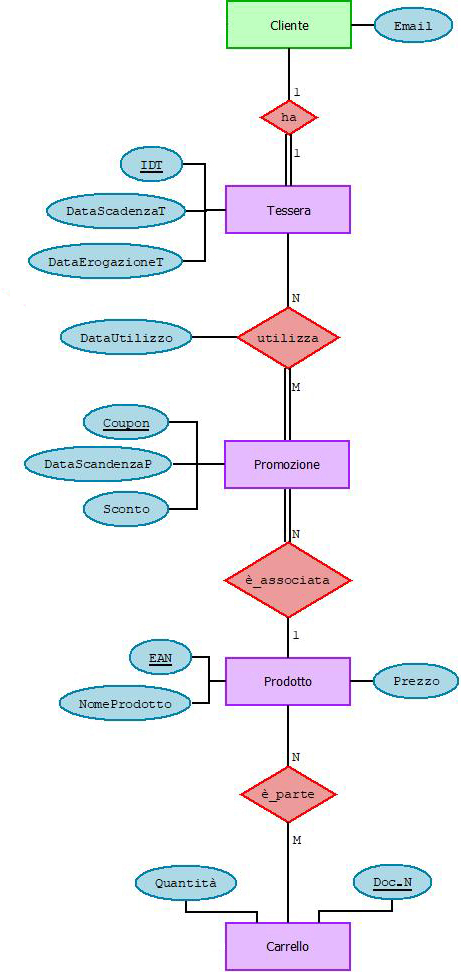
\includegraphics[scale=0.8]{imgs/eer_cliente.jpeg}
\caption{EE/R Tesseramento e Promozioni}
\end{figure}


\begin{figure}[H]
\centering
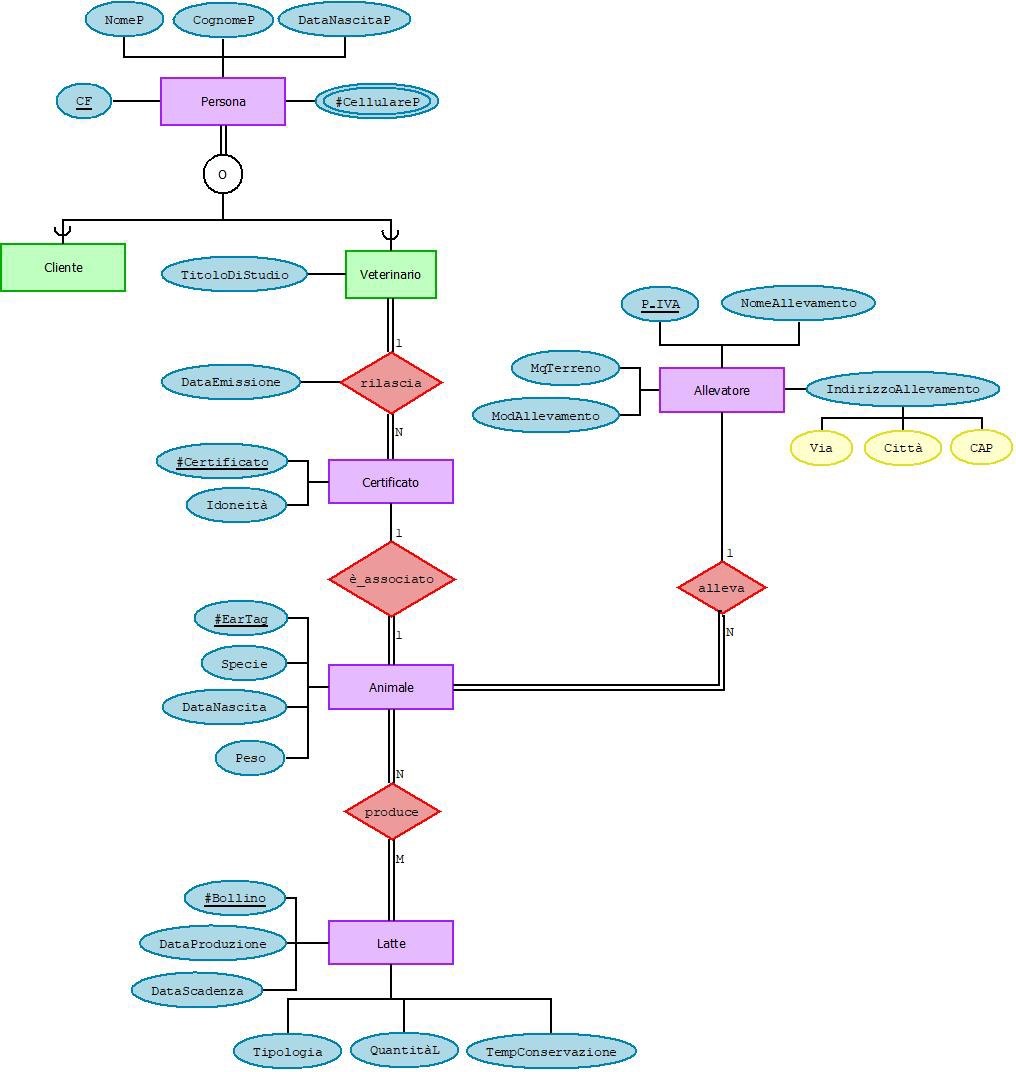
\includegraphics[scale=0.70,angle=0]{imgs/eer_veterinario.jpeg}
\caption{EE/R Gestione Animali e Latte}
\end{figure}

\begin{figure}[H]
\centering
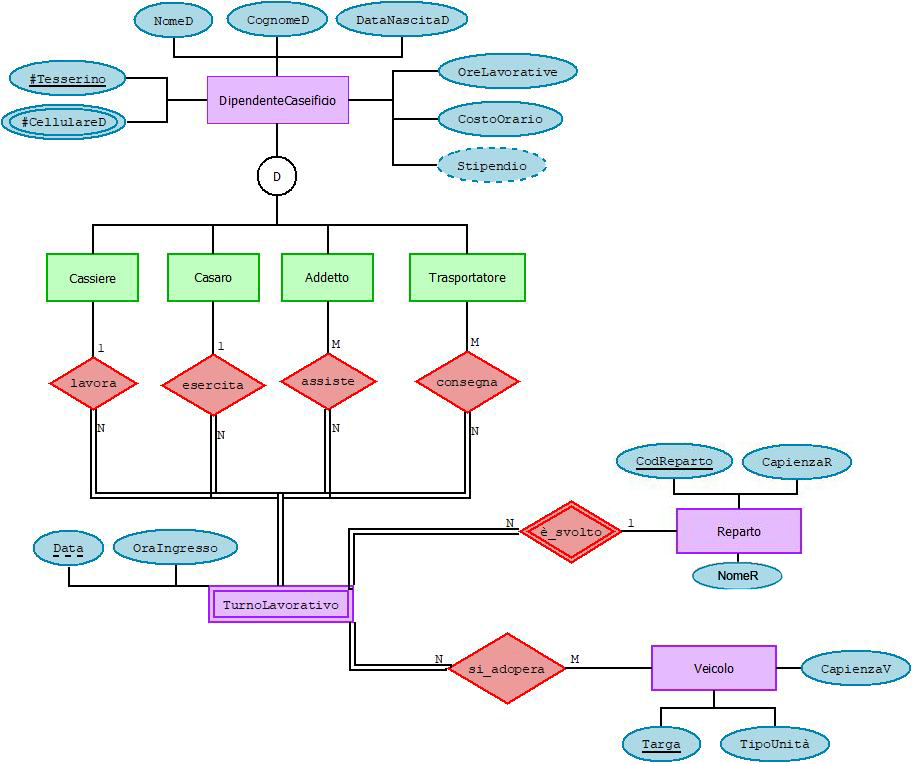
\includegraphics[scale=0.80,angle=90]{imgs/eer_dipendenti.jpeg}
\caption{EE/R Dipendenti Caseificio}
\end{figure}

\begin{figure}[H]
\centering
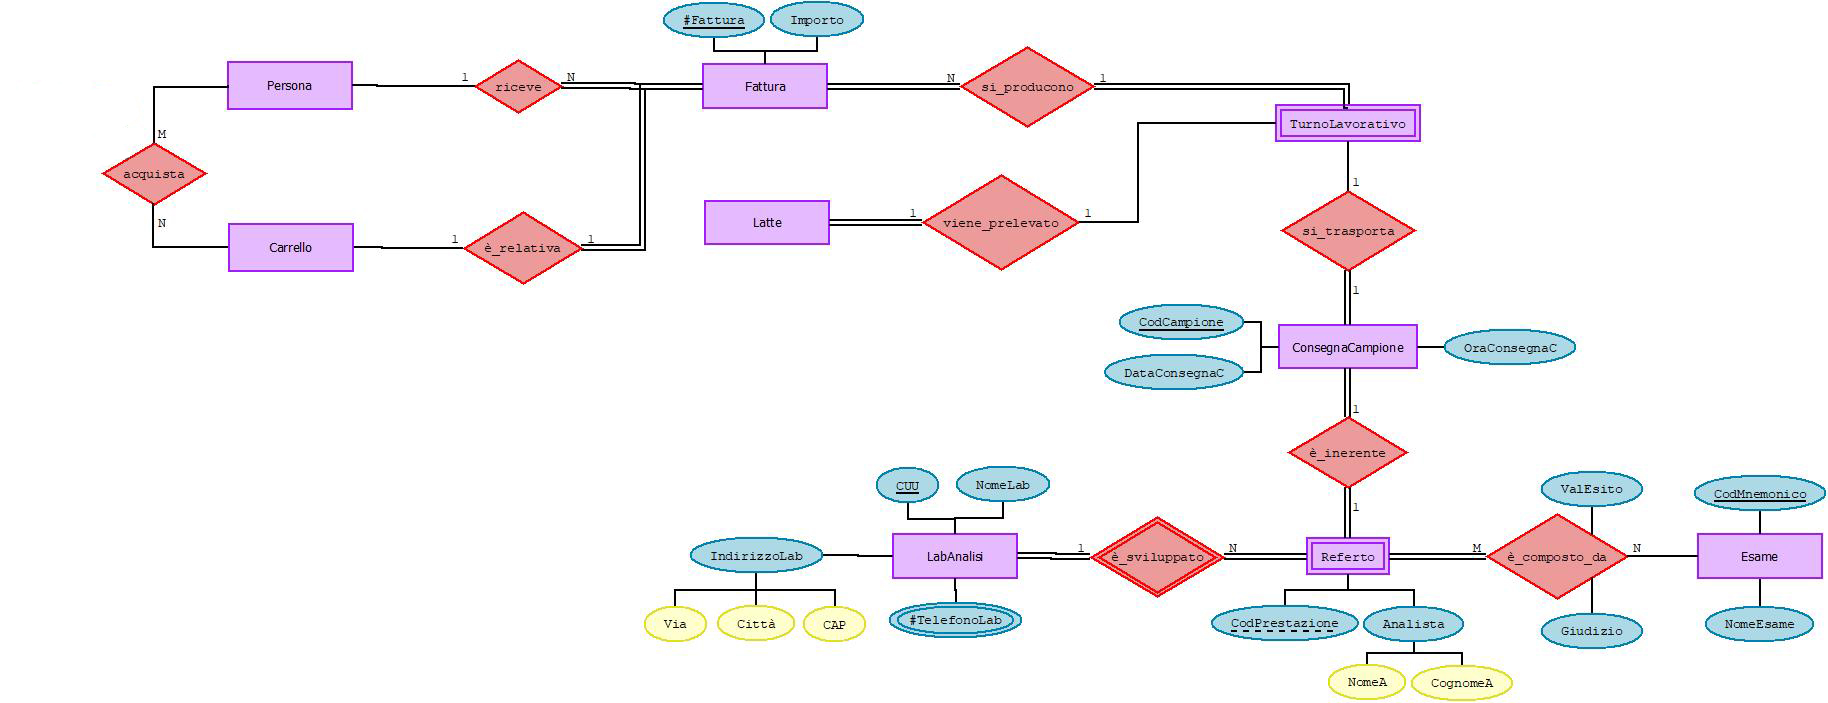
\includegraphics[scale=0.45,angle=90]{imgs/eer_LabAnalisi.jpeg}
\caption{EE/R Laboratorio Analisi e gestione Fatture}
\end{figure}

\begin{figure}[H]
\centering
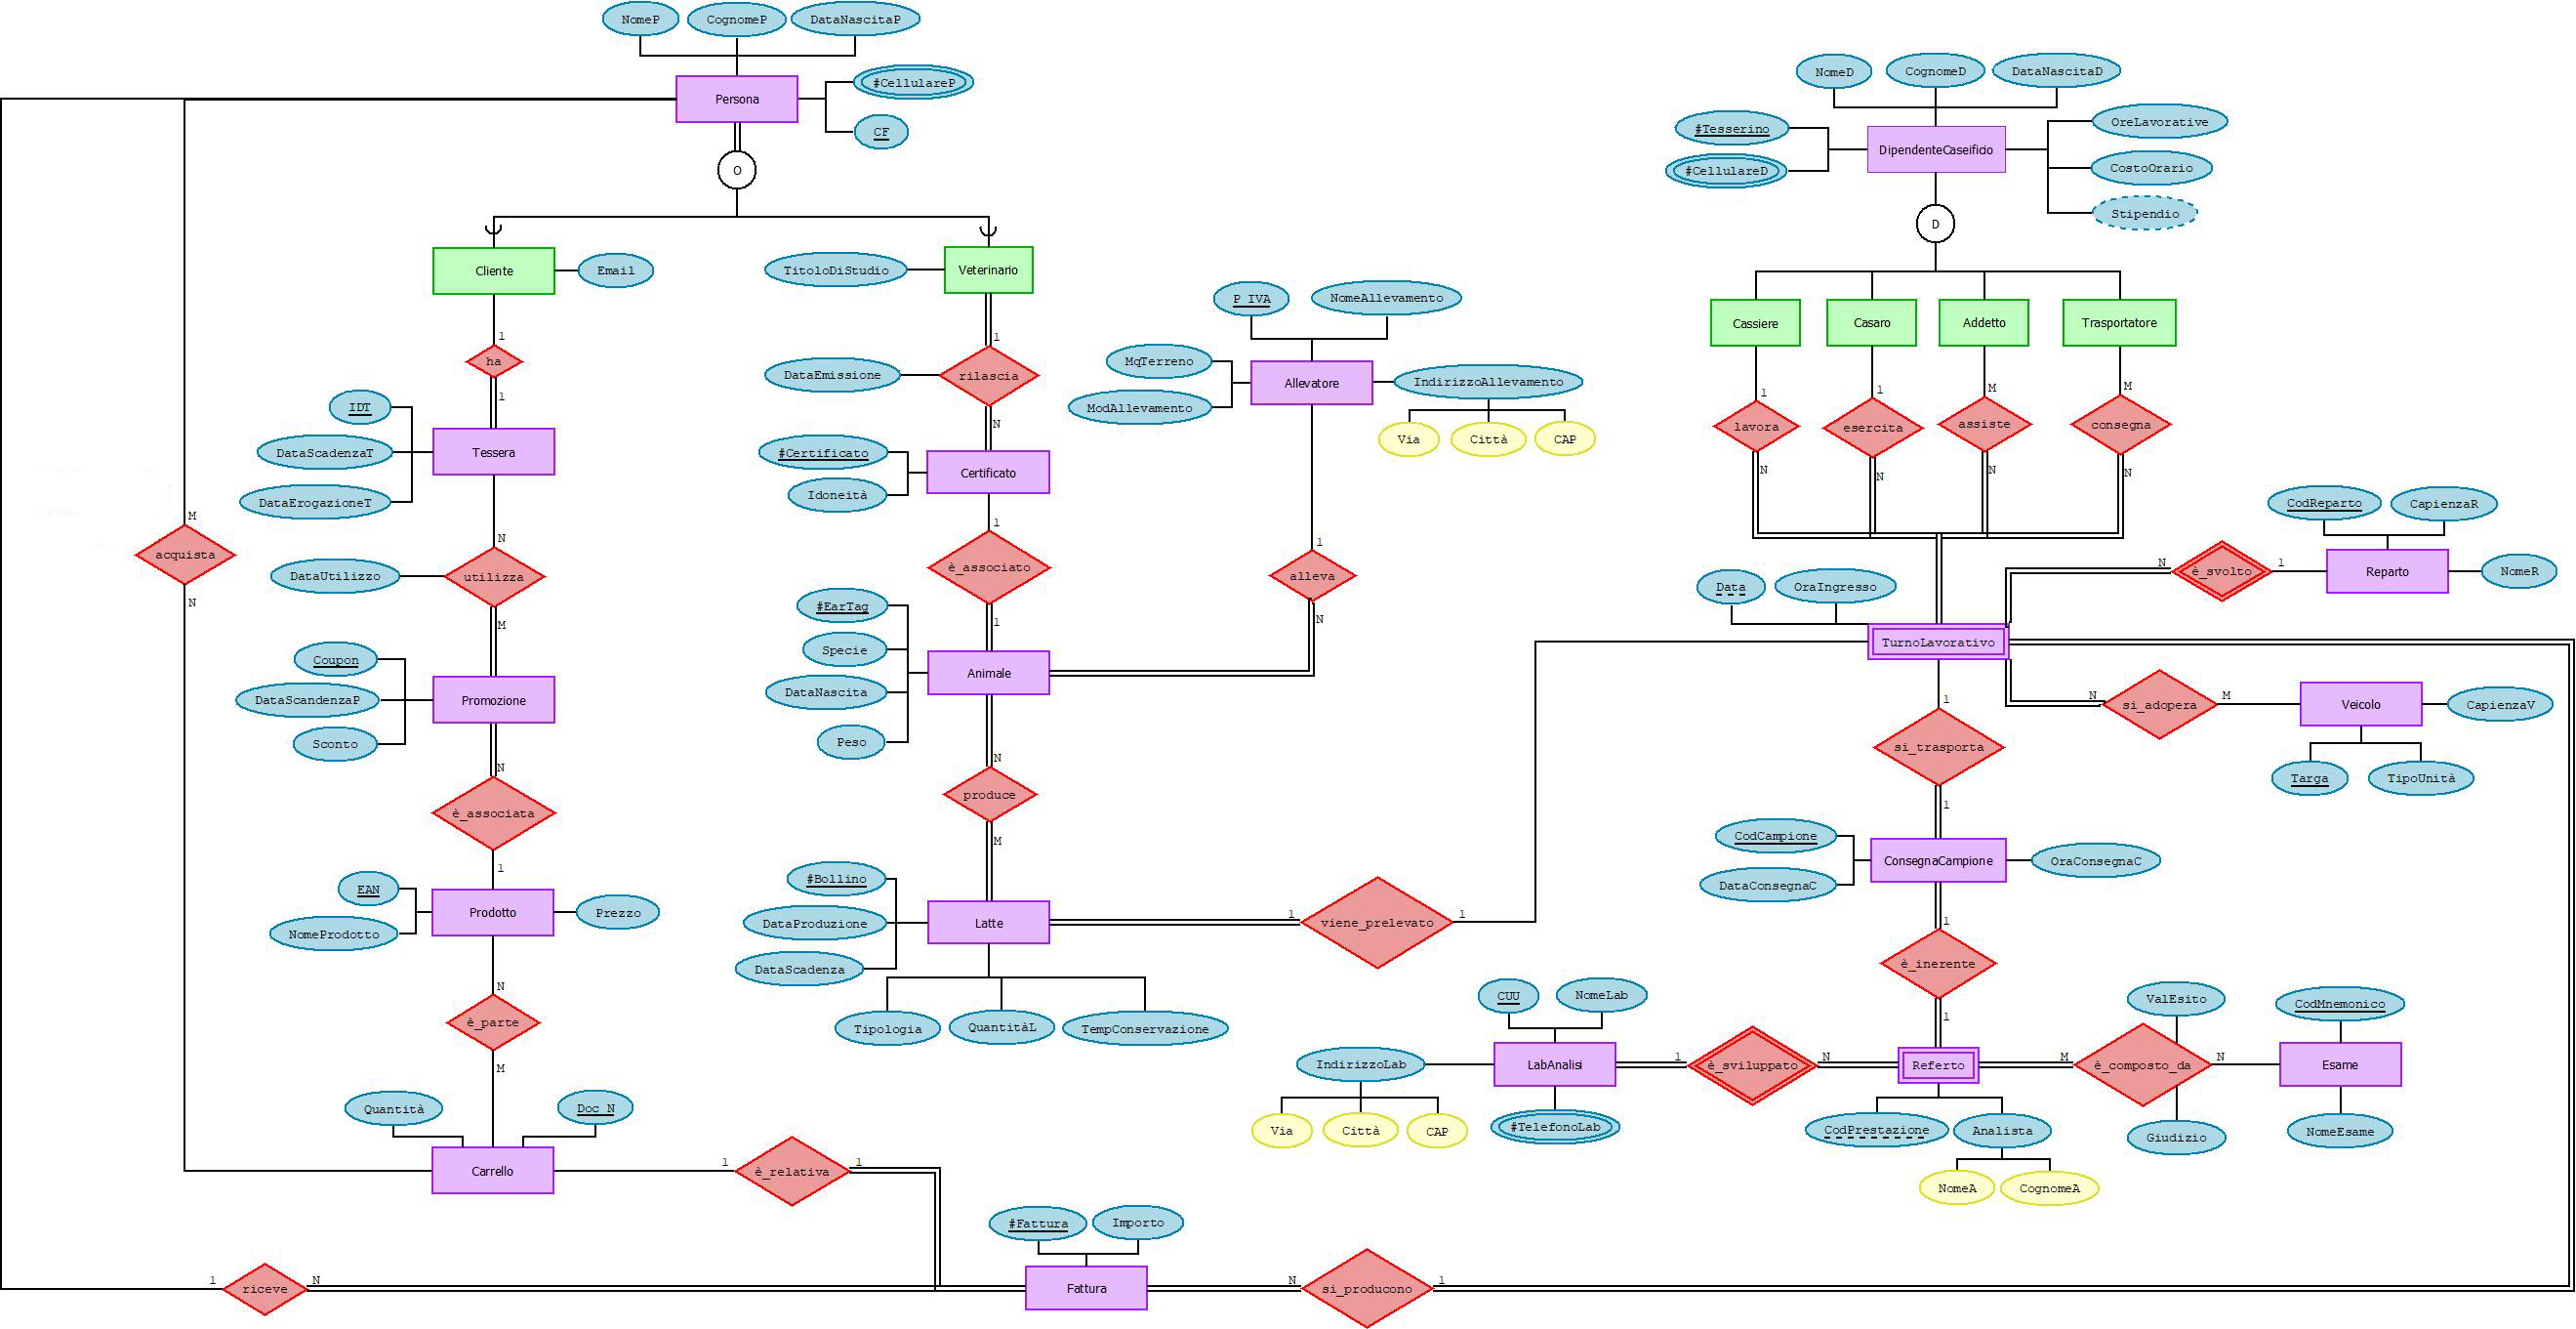
\includegraphics[scale=0.33,angle=90]{imgs/eer_completo.jpeg}
\caption{EE/R Completo}
\end{figure}



% ANALISI ENTITA'

\subsection{Analisi entità}
Di seguito verranno elencate le entità appartenenti al diagramma EE/R andando a definire il loro ruolo nel nostro mini-mondo e il significato dei loro attributi.

\begin{itemize}

\item \textbf{Persona} (\underline{CF}, NomeP, CognomeP, DataNascitaP, \#CellulareP) \\
descrive l'insieme di persone coinvolte per il sostenimento dell'attività.
\begin{itemize}
	\item CF: codice fiscale della persona (PK).
	\item NomeP: indica il nome della persona.
	\item CognomeP: indica il cognome della persona.
	\item DataNascitaP: indica la data di nascita della persona.
	\item \#CellulareP: definito come attributo multivalore, in quanto si presume che una persona possa avere più numeri di cellulare.
\end{itemize}
In merito all'entità Persona, è stato scelto di implementare una specializzazione, ovvero 2 sottoclassi (non disgiunte) che rappresentano rispettivamente i clienti e i veterinari. Si noti che essendo non disgiunte, possiamo affermare che un cliente può assumere anche il ruolo di veterinario, e viceversa.

\begin{list}{$\circ$}{}  
\item \textbf{Cliente} (Email):\\
Descrive i clienti che effettuano acquisti nel caseificio.

\begin{itemize}
\item Email: fornita dal cliente per ricevere eventuali sconti sui prodotti della società.

\end{itemize}

\item \textbf{Veterinario} (TitoloDiStudio):\\
descrive il veterinario avente il compito di visitare l'animale. 

\begin{itemize}
\item TitoloDiStudio: attestato, rilasciato dall'autorità scolastica o accademica ad una persona fisica, il quale certifica il titolo di studio conseguito dal veterinario. 

\end{itemize}
\end{list}

\item \textbf{Tessera} (\underline{IDT}, DataErogazioneT, DataScadenzaT):\\
descrive la possibilità di assegnare ad ogni cliente una tessera al fine di ottenere sconti e promozioni. La tessera viene rilasciata durante il primo acquisto o alla richiesta del cliente stesso. Questa ha una data di erogazione per tracciare quando è stata creata ed una relativa data di scadenza.
\begin{itemize}
\item IDT: acronimo di Identificativo Documento Tesserato, rilasciato dal caseificio. Permette di identificare univocamente le tessere (PK). 
\item DataErogazioneT: serve per indicare la data in cui è stata erogata la tessera al cliente.
\item DataScadenzaT: data di scadenza della tessera, la quale dovrà essere richiesta nuovamente. La tessera è valida se il cliente ha effettuato almeno un acquisto presso il caseificio.
\end{itemize}
 

\item \textbf{Promozione} (\underline{Coupon}, DataScadenzaP, Sconto):\\
descrive una determinata promozione attribuita ad uno specifico prodotto. 
\begin{itemize}
\item Coupon: buono acquisto, considerato come identificatore alfanumerico (PK), associato alle promozione di specifici prodotti caseari.
\item DataScadenzaP: identifica la scadenza della promozione. 
\item Sconto: riduzione di prezzo relativo al prodotto venduto in caseificio. 
\end{itemize}

\item \textbf{Prodotto} (\underline{EAN}, NomeProdotto, Prezzo):\\
descrive un determinato prodotto caseario. 
\begin{itemize}
\item EAN: acronimo di European Article Number, rappresenta un codice a barre utilizzato per l'identificazione univoca (PK) di prodotti destinati al consumatore finale.
\item NomeProdotto: determinata il nome del prodotto relativo alla promozione. 
\item Prezzo: identifica il prezzo relativo al prodotto. 
\end{itemize}
 
 \item \textbf{Carrello} (\underline{DOC\_N}, Quantità):\\
Carrello del cliente contenente i prodotti acquistati.
\begin{itemize}
\item {DOC\_N}: numero di documento univoco (PK), definisce l'ID dello scontrino.
\item Quantità:  attributo che identifica il numero di articoli acquistati.
\end{itemize}

\item \textbf{Fattura}(\underline{\#Fattura}, Importo):\\
fattura elettronica emessa dall'attività e consegnata al cliente.
\begin{itemize}
\item \#Fattura: identificatore alfanumerico(PK) associato ad ogni fattura emessa dal caseificio. 
\item Importo: descrive la cifra spesa dal singolo cliente.
\end{itemize}

\item \textbf{Allevatore} (\underline{P\_IVA}, NomeAllevamento, MqTerreno, ModAllevamento, IndirizzoAllevamento):\\
descrive l'azienda allevatrice di fiducia che alleva gli animali che producono latte per il continuo dell'attività casearia.
\begin{itemize}
\item P\_IVA: sequenza di 11 cifre che identifica univocamente (PK) un soggetto che esercita un'attività. 
\item NomeAllevamento: descrive il nome dell'attività di proprietà dell'allevatore.
\item MqTerreno: descrive i mq del terreno dell'azienda allevatrice.
\item ModAllevamento: descrive in che modo vengono allevati gli animali d'interesse per la società (intensivo o estensivo).
\item IndirizzoAllevamento: definito come attributo strutturato, in quanto esso può essere suddiviso in Via, CAP, Città. Tutto è in riferimento all'indirizzo dell'azienda allevatrice.
\end{itemize}

\item \textbf{Certificato} (\underline{\#Certificato}, Idoneità):\\
rilasciato dal veterinario dove vengono indicate le visite effettuato sull'animale, restituendo esito positivi o negativo.
\begin{itemize}
\item {\#Certificato}: attributo univoco (PK) che permette il riconoscimento del certificato.
\item Idoneità: attributo che indica se la visita è stata superata (T=TRUE) o meno (F=FALSE).\\
\end{itemize}

\item \textbf{Animale} (\underline{\#EarTag}, Specie, DataNascita, Peso):\\
Descrive il fulcro dell’attività: l’animale. Esso viene allevato da aziende di fiducia aventi il compito di produrre latte adibito alla realizzazione dei prodotti caseari
\begin{itemize}
\item \#EarTag: cartellino posto sull’orecchio dell’animale che  lo identifica univocamente (PK).
\item Specie: descrive la specie di un animale (bovino, ovino, caprino)
\item DataNascita: descrive la data di nascita dell’animale.
\item Peso: descrive il peso dell'animale, espresso in kg.
\end{itemize}

\item \textbf{Latte }(\underline{\#Bollino}, DataProduzione, DataScadenza, TempConservazione, QuantitàL, Tipologia):\\
Descrive il latte prodotto dagli animali che verrà processato dai macchinari dell’attività e sarà trasformato in prodotti alimentari.

\begin{itemize}
\item \#Bollino: descrive il numero di lotto univocamente (PK) di latte.
\item DataProduzione: descrive la data di produzione del latte.
\item DataScadenza: descrive la data di scadenza del latte.
\item TempConservazione: descrive la temperatura con la quale il latte viene conservato.
\item QuantitàL: esprime la quantità di latte espressa in Litri.
\item Tipologia: specifica di che tipo di latte trattato (latte bovino, latte ovino e latte caprino).
\end{itemize}

\item \textbf{DipendenteCaseificio} (\underline{\#Tesserino}, \#CellulareD, NomeD, CognomeD, DataNascitaD, OreLavorative, CostoOrario, Stipendio):\\
Indica l’insieme dei dipendenti che lavorano nel caseificio.
\begin{itemize}
\item \#Tesserino: codice alfanumerico univoco (PK) posto sul tesserino del dipendente per identificarlo.
\item \#CellulareD: definito come attributo multivalore, in quanto si presume che un dipendente possa avere più numeri di cellulare.
\item NomeD: indica il nome del dipendente.
\item CognomeD: indica il cognome del dipendente.
\item DataNascitaD: indica la data di nascita del dipendente.
\item OreLavorative: indica l'orario settimanale complessivo del lavoro svolto dal dipendente.
\item CostoOrario: indica il prezzo di un’ora lavorativa del dipendente.
\item Stipendio:  attributo derivato dalle ore lavorative e dal costo orario, indica lo stipendio mensile che percepisce il dipendente.

\end{itemize}
\item \textbf{TurnoLavorativo} ({\dashuline{\#Data}}, OraIngresso):\\
Descrive una forma di organizzazione dell’orario lavorativo, dove i lavoratori operano in una specifica data ed orario di ingresso. Tale entità rappresenta un’entità debole in quanto le sue istanze sono accettate nel sistema, se e solo se, sono presenti determinate istanze di un’altra entità da cui dipendono. In particolar modo, si fa riferimento all’entità forte Reparto.  
\begin{itemize}
\item Data: attribuito che indica la data di ingresso del turno lavorativo.
\item OraIngresso: attributo che indica l’ora di ingresso del turno lavorativo.
\end{itemize}

\item \textbf{Reparto} (\underline{CodReparto}, CapienzaR, NomeR):\\
Descrive il reparto in cui operano i dipendenti del caseificio. Ogni reparto ha un numero massimo di persone.
\begin{itemize}
\item CodReparto: attributo che specifica univocamente (PK) un determinato reparto.
\item CapienzaR: attributo che indica quante persone al più può contenere un reparto.
\item NomeR: attributo che indica il nome del reparto.
\end{itemize}

\item \textbf{Veicolo} (\underline{Targa}, CapienzaV, TipoUnità):\\
Il veicolo viene utilizzato dal trasportatore del caseificio, il quale preleva il latte dagli allevamenti, prende un campione e lo porta al laboratorio di analisi e infine porta il latte in sede.
\begin{itemize}
\item Targa: placca in materiale metallico o plastico, attributo univoco (PK) che riconosce un veicolo.
\item CapienzaV: indica quanti Litri di latte può trasportare al più il veicolo.
\item TipoUnità: indica il tipo di veicolo (Autocarri, Cisterne, Rimorchi e Scarrabili...).

\end{itemize}

\item \textbf{ConsegnaCampione} (\underline{CodCamp}, DataConsegnaC, OraConsegnaC):\\
Entità che descrive l'attività di consegna del campione al laboratorio analisi.
\begin{itemize}
\item CodCamp: attributo univoco (PK) che individua la consegna.
\item DataConsegnaC: indica la data di consegna del campione.
\item  OraConsegnaC: indica l'ora di consegna del campione.
\end{itemize}



\item \textbf{LabAnalisi} (\underline{CUU}, NomeLab, IndirizzoLab, \#TelefonoLab):\\
	Descrive il laboratorio di analisi che analizza i campioni di latte ricevuti dal trasportatore ed esegue le dovute analisi.
	\begin{itemize}
		\item CUU: acronimo di Codice Univoco Ufficio, il quale permette l’ individuazione univoca(PK), mediante codice alfanumerico, dei centri di laboratorio analisi.
		\item NomeLab: identifica il nome del laboratorio di analisi.
		\item IndirizzoLab: definito come attributo strutturato, in quanto esso è suddiviso in Via, Cap e Città. Fa riferimento all’indirizzo del laboratorio di analisi di campioni di latte.
		\item \#TelefonoLab: definito come attributo multivalore, in quanto si presume che un laboratorio possa avere più contatti telefonici.

	\end{itemize}
	
	\item \textbf{Referto} (\dashuline{CodPrestazione}, Analista):\\
Relazione scritta e analizzata da un analista che stabilisce l’esito positivo delle analisi dopo una serie di esami standard di routine. Tale entità è debole in quanto le sue istanze sono accettate nel sistema, se e solo se, sono presenti determinate istanze di un’altra entità da cui dipendono. In questo particolare caso, si fa riferimento al LabAnalisi.
	\begin{itemize}
		\item CodPrestazione: definito come attributo di chiave debole, rappresenta un codice che identifica un referto specifico.
	    \item Analista: definito come attributo strutturato, in quanto sul referto è possibile riportare il nome e cognome dell’analista che ha effettuato la convalida. 
	\end{itemize}
\item \textbf{Esame} (\underline{CodMnemonico}, NomeEsame):\\
Definito come l’insieme degli esami clinici che fanno parte dei singoli referti prodotti.
	\begin{itemize}
		\item CodMnemonico: composto da valori alfanumerici, permette di identificare univocamente (PK) gli esami clinici. 
	    \item NomeEsame: indica il nome dell'esame eseguito.
	\end{itemize}

\item \textbf{è\_composta\_da} (ValEsito, Giudizio):\\
rappresenta una tabella che deriva dalla molteplicità M:N tra Referto ed Esame.
	\begin{itemize}
		\item ValEsito: indica il valore numerico dell’esito, prodotto durante gli esami clinici svolti.
		\item Giudizio: indica la valutazione dell'esame positiva (pos) o negativa (neg).
	\end{itemize}

\item \textbf{utilizza} (DataUtilizzo):\\
rappresenta una tabella che deriva dalla molteplicità M:N tra Tessera e Promozione.
	\begin{itemize}
		\item DataUtilizzo: rappresenta la data utilizzo della tessera utilizzata per l'acquisto di prodotti effettuati dal cliente.
	\end{itemize}

\end{itemize}

% FINE ANALISI ENTITA'

% ANALISI ASSOCIAZIONI

\subsection{Analisi associazioni}
L’analisi delle associazioni va a definire il significato delle relazioni, la scelta di una determinata molteplicità e totalità. Di seguito sono elencate le associazioni presenti nello schema, del perché esistono e cosa rappresentano.

\begin{itemize}
\item \textbf{(Cliente, Tessera)}
	\begin{itemize}
		\item \underline{Molteplicità (1:1 - Biunivoca)}  \\ [2mm]
			Un cliente ha una sola tessera. \\ 
			Ogni tessera è associata a un solo cliente. \\
		\item \underline{Totalità} \\ [2mm]
		        Non tutti i clienti hanno una tessera.\\
                Ogni tessera è assegnata a un cliente.

	\end{itemize}
\item \textbf{(Tessera, Promozione) }
	\begin{itemize}
		\item \underline{Molteplicità (N:M - Multivalore Doppia) } \\ [2mm]
			Una tessera può essere utilizzata per più promozioni. \\ 
			La stessa promozione può essere disponibile per più tessere. \\
		\item \underline{Totalità} \\ [2mm]
			Non tutte le tessere sono abilitate a promozioni. \\ 
		Tutte le promozioni sono utilizzate dalle tessere.
	\end{itemize}

\newpage

\item \textbf{(Promozione, Prodotto)} 
	\begin{itemize}
		\item \underline{Molteplicità (N:1 - Univoca)} \\ [2mm]
		   	Una promozione è associata a una categoria di prodotti.\\
             Un prodotto è associato a più promozioni.\\

		\item \underline{Totalità} \\ [2mm]
			Tutte le promozioni sono associate a prodotti.\\
            Non tutti i prodotti sono associati a promozioni.\\
	\end{itemize}

\item \textbf{(Prodotto, Carrello)} 
	\begin{itemize}
		\item \underline{Molteplicità (N:M - Multivalore Doppia)} \\ [2mm]
			Una categoria di prodotti è parte di più carrelli.\\
            Un carrello può contenere più prodotti.\\

		\item \underline{Totalità} \\ [2mm]
			Non tutti i prodotti sono assegnati a carrelli.\\
            Non tutti i carrelli contengono prodotti.\\
	\end{itemize}	
	
\item \textbf{(Persona, Carrello)} 
	\begin{itemize}
		\item \underline{Molteplicità (M:N - Multivalore Doppia) } \\ [2mm]
			Una persona utilizza più carrelli per l'acquisto.\\
            Un carrello può essere utilizzato da differenti persone.\\ 

		\item \underline{Totalità} \\ [2mm]
        	Non tutte le persone acquistano prodotti contenuti nei carrelli.\\
            Non tutti i carrelli sono utilizzati per gli acquisti da persone.\\

	\end{itemize}
\item \textbf{(Persona, Fattura)} 
	\begin{itemize}
		\item \underline{Molteplicità (1:N - Multivalore) } \\ [2mm]
	    	Una persona può riceve più fatture.\\
            Una fattura è associata ad una persona.\\

		\item \underline{Totalità} \\ [2mm]
		    Non tutte le persone effettuano acquisti e, di conseguenza, non tutti ricevono fatture.\\
            Tutte le fatture sono associate a persone.\\
	\end{itemize}
	
\newpage
	
\item \textbf{(Carrello, Fattura)} 
	\begin{itemize}
		\item \underline{Molteplicità (1:1 - Biunivoca) } \\ [2mm]
	    	Un carrello è associato ad una fattura.\\
            Una fattura è associata ad un carrello.\\

		\item \underline{Totalità} \\ [2mm]
		    Non tutti i prodotti presenti nei carrelli sono relative ad una fattura.\\
            Tutte le fatture sono associate a determinati acquisiti mediante carrelli.\\
	\end{itemize}

\item \textbf{(Fattura, TurnoLavorativo)} 
	\begin{itemize}
		\item \underline{Molteplicità (N:1 - Univoca) } \\ [2mm]
	    	Un fattura viene emessa durante un turno lavorativo.\\
            In un turno lavorativo possono essere emesse più fatture.\\

		\item \underline{Totalità} \\ [2mm]
		    Tutte le fatture sono prodotte durante un turno lavorativo.\\
            In tutti i turni lavorativi vengono prodotte fatture.\\
	\end{itemize}

\item \textbf{(Veterinario, Certificato)}
	\begin{itemize}
		\item \underline{Molteplicità (1:N - Multivalore)} \\ [2mm]
		Un veterinario rilascia più certificati. \\
        Un certificato è rilasciato da un veterinario. \\

		\item \underline{Totalità} \\ [2mm]
			Tutti i veterinari rilasciano certificati. \\
            Tutti i certificati sono rilasciati da veterinari. \\
	\end{itemize}
	
\item \textbf{(Certificato, Animale)} 
	\begin{itemize}
		\item \underline{Molteplicità (1:1 - Biunivoca) } \\ [2mm]
			Un certificato è relativo a un animale.\\
			Un animale possiede un certificato.\\
            
		\item \underline{Totalità} \\ [2mm]
			Non tutti i certificati sono associati ad animali.\\
			Tutti gli animali hanno un certificato.\\
	\end{itemize}

\newpage
	
\item \textbf{(Allevatore, Animale)} 
	\begin{itemize}
		\item \underline{Molteplicità (1:N - Multivalore) } \\ [2mm]
			Un allevatore può allevare più di un animale.\\
			Un animale è allevato da un solo allevatore.\\
            
		\item \underline{Totalità} \\ [2mm]
			Non tutti gli allevatori allevano animali.\\
			Tutti gli animali vengono allevati da un allevatore.\\
	\end{itemize}
	
\item \textbf{(Animale, Latte) }
	\begin{itemize}
		\item \underline{Molteplicità (N:M - Multivalore Doppia)} \\ [2mm]
			Un animale produce diversi litri di latte.\\
            Il latte è prodotto da più animali.\\

		\item \underline{Totalità} \\ [2mm]
			Tutti gli animali producono latte.\\
            Tutto il latte è prodotto da animali.\\
	\end{itemize}
	
\item \textbf{(Latte, TurnoLavorativo) }
	\begin{itemize}
		\item \underline{Molteplicità (1:1 - Biunivoca) } \\ [2mm]
			Una certa quantità di latte viene prelevata durante un turno lavorativo.\\
            Durante un turno lavorativo si prelevano determinate quantità di latte.\\

		\item \underline{Totalità} \\ [2mm]
			Tutte le quantità di latte vengono prelevate durante un turno lavorativo.\\
            Durante non tutti i turni lavorativi si prelevano quantità di latte.\\
	\end{itemize}

\item \textbf{(Cassiere, TurnoLavorativo) }
	\begin{itemize}
		\item \underline{Molteplicità (1:N - Multivalore) } \\ [2mm]
			Un cassiere può lavorare in più turni lavorativi.\\
            Durante un turno lavorativo lavora un solo cassiere.\\

		\item \underline{Totalità} \\ [2mm]
			Non tutti i cassieri lavorano in turni lavorativi.\\
            In tutti i turni lavorativi lavora un cassiere.\\
	\end{itemize}

\newpage	

\item \textbf{(Casaro, TurnoLavorativo) }
	\begin{itemize}
		\item \underline{Molteplicità (1:N - Multivalore) } \\ [2mm]
			Un casaro può esercitare in più turni lavorativi.\\
            Durante un turno lavorativo esercita un solo casaro.\\

		\item \underline{Totalità} \\ [2mm]
			Non tutti i casari esercitano in turni lavorativi.\\
            In tutti i turni lavorativi esercita un casaro.\\
	\end{itemize}

\item \textbf{(Addetto, TurnoLavorativo) }
	\begin{itemize}
		\item \underline{Molteplicità (M:N - Multivalore doppia) } \\ [2mm]
			Un addetto può assistere in più turni lavorativi.\\
            Durante un turno lavorativo assistono più addetti.\\

		\item \underline{Totalità} \\ [2mm]
			Non tutti gli addetti assistono in turni lavorativi.\\
            In tutti i turni lavorativi assiste almeno un addetto.\\
	\end{itemize}
	
\item \textbf{(Trasportatore, TurnoLavorativo) }
	\begin{itemize}
		\item \underline{Molteplicità (M:N - Multivalore doppia) } \\ [2mm]
			Un trasportatore può effettuare consegne in più turni lavorativi.\\
            Durante un turno lavorativo si effettuano consegne da più trasportatori.\\

		\item \underline{Totalità} \\ [2mm]
			Non tutti i trasportatori consegnano in turni lavorativi.\\
            In tutti i turni lavorativi si effettuano almeno una consegna da un trasportatore.\\
	\end{itemize}

\item \textbf{(TurnoLavorativo, Reparto) }
	\begin{itemize}
		\item \underline{Molteplicità (N:1 - Univoca) } \\ [2mm]
			Un turno lavorativo può essere svolto in un determinato reparto.\\
            In un reparto possono essere svolti più turni lavorativi.\\

		\item \underline{Totalità} \\ [2mm]
			Tutti i turni lavorativi sono svolti in dei reparti.\\
            In non tutti i reparti si svolgono turni lavorativi.\\
	\end{itemize}

\newpage

\item \textbf{(TurnoLavorativo, Veicolo) }
	\begin{itemize}
		\item \underline{Molteplicità (N:M - Multivalore doppia) } \\ [2mm]
			In un turno lavorativo si adoperano più veicoli per le consegne.\\
            Un veicolo può essere adoperato durante più turni lavorativi.\\

		\item \underline{Totalità} \\ [2mm]
			In tutti i turni lavorativi si adoperano veicoli. \\
            Non tutti i veicoli vengono utilizzati durante turni lavorativi.\\
	\end{itemize}

\item \textbf{(TurnoLavorativo, ConsegnaCampione) }
	\begin{itemize}
		\item \underline{Molteplicità (1:1 - Biunivoca) } \\ [2mm]
			In un turno lavorativo può essere trasportato un solo campione di latte.\\
            La consegna campione di latte può essere trasportata durante un turno lavorativo.\\

		\item \underline{Totalità} \\ [2mm]
			In non tutti i turni lavorativi si trasportano consegne campioni di latte.\\
		    Tutte le consegne campioni di latte vengono trasportate durante turni lavorativi.\\
	\end{itemize}

\item \textbf{(ConsegnaCampione, Referto) }
	\begin{itemize}
		\item \underline{Molteplicità (1:1 - Biunivoca) } \\ [2mm]
            La consegna campione di latte è riferita ad un referto.\\
            Un referto è inerente ad una sola consegna di campione effettuata.

		\item \underline{Totalità} \\ [2mm]
		    Tutti i campioni di latte sono inerenti a referti.\\
		    Tutti i referti fanno riferimento ad una consegna campione.
	\end{itemize}

\item \textbf{(Referto, LabAnalisi) }
	\begin{itemize}
		\item \underline{Molteplicità (N:1 - Univoca) } \\ [2mm]
            Un referto viene sviluppato in un solo laboratorio di analisi.\\
            In un laboratorio di analisi vengono sviluppati più referti.

		\item \underline{Totalità} \\ [2mm]
		    Tutti i referti sono sviluppati in un laboratorio di analisi.\\
		    Nel laboratorio di analisi si sviluppano tanti referti.
	\end{itemize}

\newpage
	
\item \textbf{(Referto, Esame) }
	\begin{itemize}
		\item \underline{Molteplicità (M:N - Multivalore Doppia) } \\ [2mm]
            Un referto è composto da più esami.\\
            Un esame è parte di più referti.\\
		\item \underline{Totalità} \\ [2mm]
		    Tutti i referti sono composti da più esami.\\
		    Non tutti gli esami fanno parte di più referti.
	\end{itemize}

\end{itemize}

\section{Schema relazionale}

\begin{figure}[H]
\centering
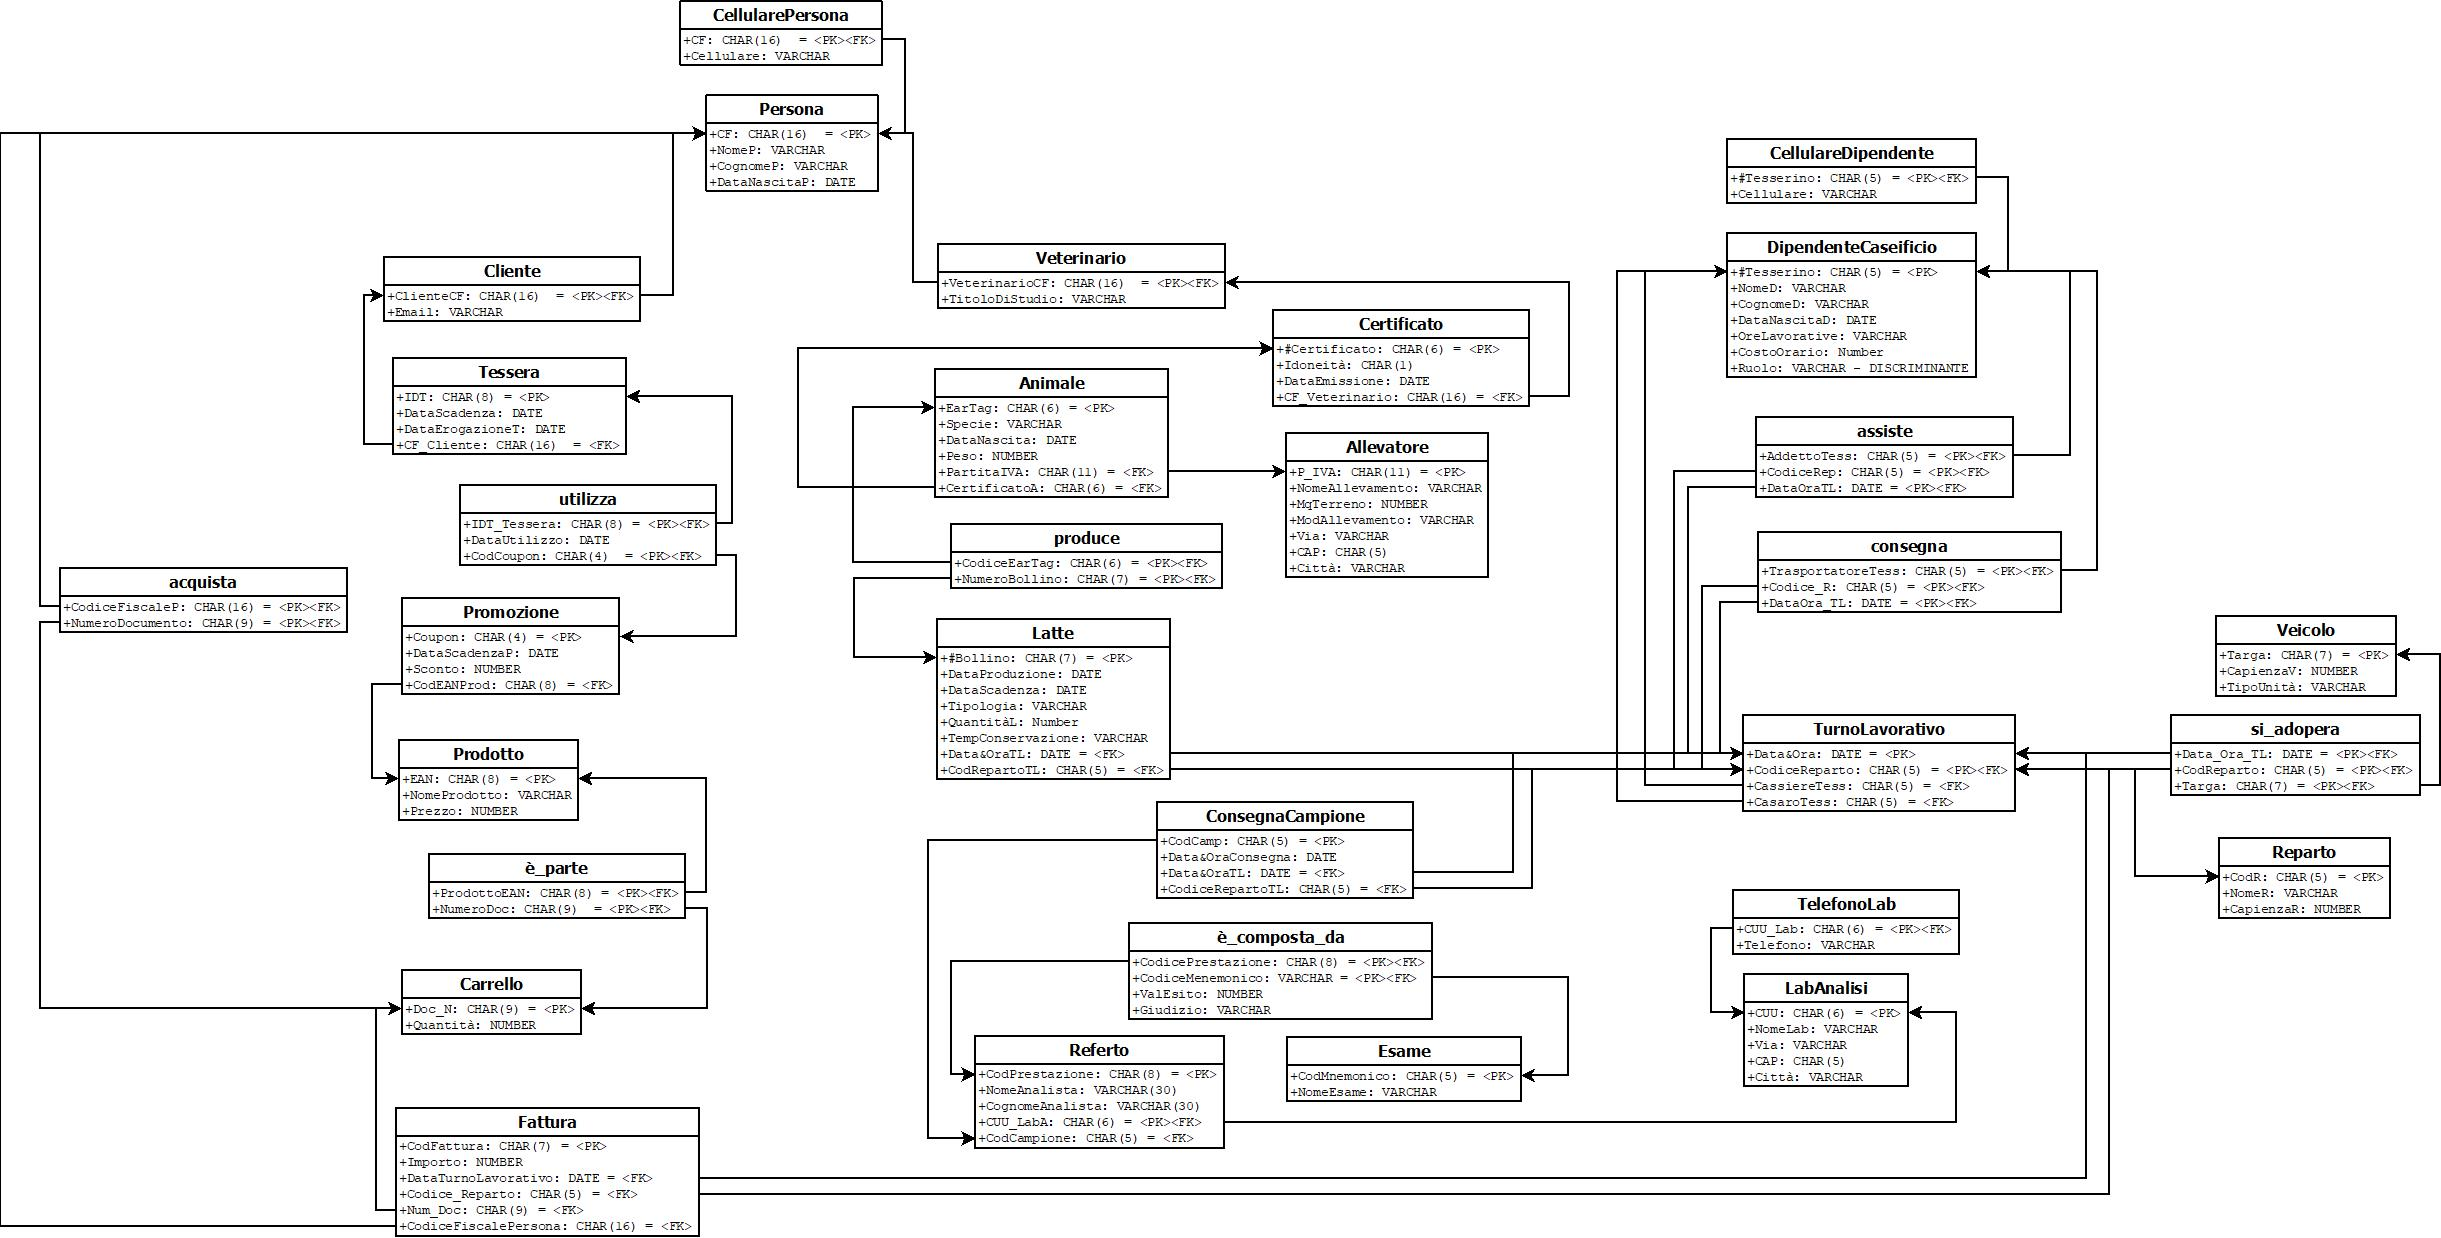
\includegraphics[scale=0.33,angle=90]{imgs/sc_relazionale.jpeg}
\caption{Schema Relazionale}
\end{figure}

% CATEGORIE DI UTENTI

\section{Utenti}
Le categorie di utenti scelti sono:
\begin{itemize}
\item {Cassiere};
\item {Casaro};
\item {Addetto};
\item {Trasportatore};
\item {Allevatore};
\item {Cliente};
\item {Analista};
\item {Veterinario}. \\
\\
Ciò non vieta che possono essere aggiunti altri utenti come un Personale ausiliario \\
 ed amministrativo per il LabAnalisi (Personale addetto all'accettazione).
\end{itemize}



% FINE CATEGORIE DI UTENTI


% PRIVILEGI DI ACCESSO

\subsection{Privilegi di accesso}

\begin{itemize}
\item {Un Cassiere può accedere ai dati relativi alla Fattura dei prodotto acquistati da un cliente, e ai dati del Turno Lavorativo}
\item {Un Casaro può accedere ai dati relativi al Turno Lavorativo, ai dati relativi ai Reparti e ai dati relativi alle Consegne campione e visualizzare i dati dei referti.}
\item {Un Addetto può accedere ai dati relativi al Turno Lavorativo, ai dati relativi ai Reparti.}
\item {Un Trasportatore può accedere ai dati relativo al Turno Lavorativo, ai dati inerenti ai Veicoli disponibili, ai prelievi del latte e alle consegne campione.}
\item {Un Allevatore può accedere ai dati relativi agli animali.}

\item {Un Cliente può accedere ai dati relativi alla Tessera, alla Promozione, al Prodotto, al Carrello e alla Fattura.}
\item {Un Analista può accedere ai dati del Laboratorio di Analisi, al Referto ed i suoi Esami, ai dati relativi alle Consegne campioni.}
\item {Un Veterinario può accedere ai dati relativi agli animali e al certificato per stabilire l'idoneità dell'animale stesso.}\\
\end{itemize}

\newpage

	% PRIVILEGI DI ACCESSO - Cassiere
\textbf{Cassiere}\\
	Il Cassiere all'interno del DB può accedere ai dati delle Fatture e dei Turni di lavoro. Si occupa della gestione della tessera, del carrello finale del cliente. Ha la possibilità di effettuare modifiche sui dati relativi ai clienti.  \\

	\begin{tabular}{ |c|c|c|c|c| }
	\hline
 			\textbf{Tabella} & \textbf{Inserimento} & \textbf{Modifica (Update)} & \textbf{Cancellazione} & \textbf{Visualizzazione}\\ 
 			\hline
 			DipendenteCaseificio & & & & X \\ 
 			\hline
 			CellulareDipendente & X & X & X & X \\ 
 			\hline
 			TurnoLavorativo  & & & & X \\ 
 			\hline
			Reparto & & & & X \\ 
			\hline
 			Persona &  &  &  & X  \\ 
 			\hline
 			CellularePersona  &  &  &  & X  \\ 
 			\hline
 			Cliente  & X & X & X & X  \\ 
 			\hline
 		    Cellulare Cliente  & X & X & X & X  \\ 
 			\hline
 			Tessera & X & & & X \\ 
 			\hline
 			utilizza & X & & & X \\ 
            \hline
 		 	Promozione &  &  &  & X \\ 
 			\hline
 			Prodotto &  &  &  & X \\ 
            \hline
            Carrello & X & X & X & X \\
            \hline
            acquista & X & & & X \\
            \hline
            Fattura & X & X & X & X \\
            \hline
\end{tabular}\\\\\\ 
	% PRIVILEGI DI ACCESSO - Casaro
	\textbf{Casaro}\\
 Il Casaro è colui che gestisce l'intera attività. All'interno del DB può visualizzare parti di informazioni ad esso importanti come: i suoi dati personali, dati relativi al Laboratorio Analisi affiliati, i referti emessi da quest'ultimo, gli esami sviluppati dai referti, il latte che viene prelevato durante il turno lavorativo, l'azienda allevatrice con i suoi animali e i certificati emessi dal veterinario. Può apportare modifiche su tutte le informazioni dei dipendenti del caseificio, gestisce gli orari di ingresso dei turni lavorativi, dei reparti e delle consegne campioni da affiliare ai laboratori analisi. Decide che promozioni applicare su quali prodotti presenti in caseificio.\\

	\begin{tabular}{ |c|c|c|c|c| }	 
	\hline
 			\textbf{Tabella} & \textbf{Inserimento} & \textbf{Modifica (Update)} & \textbf{Cancellazione} & \textbf{Visualizzazione}\\ 
 			\hline
 			DipendenteCaseificio &  &  &  & X \\ 
 			\hline
 			CellulareDipendente & X & X & X & X \\ 
 			\hline
 			TurnoLavorativo  & X & X & X & X \\ 
 			\hline
			Reparto & X & X & X & X \\ 
			\hline
			Veicolo & X & X & X & X \\ 
			\hline
 			ConsegnaCampione & X & X & X & X  \\ 
 			\hline
 			LabAnalisi  &  &  &  & X  \\ 
 			\hline
 			TelefonoLabAnalisi  &  &  &  & X  \\ 
 			\hline
 		    Referto  &  &  &  & X  \\ 
 			\hline
 			è\_composto\_da &  & & & X \\ 
 			\hline
 			Esame &  & & & X \\ 
            \hline
 		 	Latte & X & X & X & X \\ 
 			\hline
 			Promozione & X & X & X & X \\ 
            \hline
            Prodotto & X & X & X & X \\
            \hline
            Persona &  & & & X \\
            \hline
            CellularePersona &  &  &  & X \\
            \hline
            Allevatore &  &  &  & X \\
            \hline
            Animale &  &  &  & X \\
            \hline
 		    Certificato &  &  &  & X \\
            \hline
          Veterinario &  &  &  & X \\
            \hline
	\end{tabular}\\\\\\
	% PRIVILEGI DI ACCESSO - ADDETTO
	\textbf{Addetto}\\
	Un Addetto può visualizzare tutte le sue informazioni personali; visualizzare i suoi turni lavorativi e in quale reparto lavorare; visualizzare informazioni sulla tracciabilità del latte e la provenienza da quale animale. Può infine visualizzare il certificato dell'animale. \\

	\begin{tabular}{ |c|c|c|c|c| }
	 \hline
 		\textbf{Tabella} & \textbf{Inserimento} & \textbf{Modifica (Update)} & \textbf{Cancellazione} & \textbf{Visualizzazione}\\
 		\hline
	        DipendenteCaseificio &  &  &  & X \\ 
 			\hline
 			CellulareDipendente & X  &  X & X & X \\ 
 			\hline
 			TurnoLavorativo  &  &  &  & X \\ 
 			\hline
			Reparto &  &  &  & X \\ 
			\hline
 			ConsegnaCampione &  &  &  & X  \\ 
 			\hline
 			Latte &  &  &  & X  \\ 
 			\hline
 			Animale &  &  &  & X  \\ 
 			\hline
 			Certificato &  &  &  & X  \\ 
 			\hline
 			
	\end{tabular}\\\\\\
	\newpage
	% PRIVILEGI DI ACCESSO - Trasportatore
	\textbf{Trasportatore}\\
	Un Trasportatore effettua consegne durante un turno lavorativo: può visualizzare i dipendenti del caseificio e i loro dati, il turno lavorativo, il reparto coinvolto, il veicolo da utilizzare durante la consegna, le consegne di campioni da trasportare ai laboratori di analisi affiliati, il latte prelevato, le aziende allevatrici e i loro animali. \\

	\begin{tabular}{ |c|c|c|c|c| }
	 \hline
 		\textbf{Tabella} & \textbf{Inserimento} & \textbf{Modifica (Update)} & \textbf{Cancellazione} & \textbf{Visualizzazione}\\
	 \hline
        	DipendenteCaseificio &  &  &  & X \\ 
 			\hline
 			CellulareDipendente & X  &  X & X & X \\ 
 			\hline
 			TurnoLavorativo  &  &  &  & X \\ 
 			\hline
			Reparto &  &  &  & X \\ 
			\hline
			Veicolo &  &  &  & X \\ 
			\hline
 			ConsegnaCampione &  &  &  & X  \\ 
 			\hline
 			LabAnalisi &  &  &  & X \\ 
			\hline
		    TelefonoLabAnalisi &  &  &  & X \\ 
			\hline
			Allevatore &  &  &  & X \\ 
			\hline
 			Latte &  &  &  & X  \\ 
 			\hline
 			Animale &  &  &  & X  \\ 
 			\hline
 		
	\end{tabular}\\\\\\
	% PRIVILEGI DI ACCESSO - Allevatore	
	\textbf{Allevatore}\\
	Azienda agricola-animale che si occupa dell'allevamento di determinate specie. Può modificare e visualizzare i propri dati, gli animali allevati e il latte prodotto da questi ultimi. Può visualizzare i dati relativi al veterinario e ai certificati da esso rilasciato. \\

	\begin{tabular}{ |c|c|c|c|c| }
	 \hline
 		\textbf{Tabella} & \textbf{Inserimento} & \textbf{Modifica (Update)} & \textbf{Cancellazione} & \textbf{Visualizzazione}\\
	 \hline
			Allevatore & X & X & X & X \\ 
			\hline
 			Latte & X & X & X & X  \\ 
 			\hline
 			Animale & X & X & X & X  \\ 
 			\hline
 		    Veterinario &  &  &  & X  \\ 
 			\hline
	        Certificato &  &  &  & X  \\ 
 			\hline 			
 			  Persona &  & & & X \\
            \hline
            CellularePersona &  &  &  & X \\
            \hline
 	\end{tabular}\\\\\\

\newpage

	% PRIVILEGI DI ACCESSO - Cliente	
\textbf{Cliente}\\
	Il Cliente è colui che effettua acquisti presso il caseificio. Può visualizzare le sue informazioni personali, i dati relativi alla Tessera, le promozioni disponibili, la fattura ricevuta e la data di acquisto dei prodotti.\\

	\begin{tabular}{ |c|c|c|c|c| }
	 \hline
 		\textbf{Tabella} & \textbf{Inserimento} & \textbf{Modifica (Update)} & \textbf{Cancellazione} & \textbf{Visualizzazione}\\
	 	\hline
 		Persona & & & & X \\ 
 		\hline
 		CellularePersona & X & X & X & X \\ 
 		\hline
 		Cliente & X & X & & X \\ 
 		\hline
 		Tessera & & & & X \\ 
 		\hline
 		utilizza & & & & X \\ 
 		\hline
 		Promozione & & & & X \\ 
 		\hline
 		Prodotto & & & & X \\ 
 		\hline
 		Carrello & X & X & & X \\ 
 		\hline
 		Fattura & X & X & X & X \\ 
 		\hline
 		acquista & X & X & X & X \\ 
 		\hline
	\end{tabular}\\\\\\
	\textbf{Analista}\\
        L'analista si occupa della formulazione del referto inerente al latte consegnato. Può effettuare modifiche e visualizzazioni sul valore del referto e sugli esami ottenuti.\\

	\begin{tabular}{ |c|c|c|c|c| }
	 \hline
 		\textbf{Tabella} & \textbf{Inserimento} & \textbf{Modifica (Update)} & \textbf{Cancellazione} & \textbf{Visualizzazione}\\
	 	\hline
        	ConsegnaCampione &  &  &  & X  \\ 
 			\hline
 			LabAnalisi &  &  &  & X \\ 
			\hline
		    TelefonoLabAnalisi &  &  &  & X \\ 
			\hline
			Referto & X & X & X & X \\ 
			\hline
 			è\_composto\_da & X & X & X & X  \\ 
 			\hline
 			Esame & X & X & X & X  \\ 
 			\hline
 		    Latte &  &  &  & X  \\ 
 			\hline
 			
	        \end{tabular}\\\\\\
	\textbf{Veterinario}\\
	Il Veterinario è colui che effettua le visite di routine per il controllo degli animali. Può modificare e visualizzare i suoi dati e i certificati. Può visualizzare i dati relativi agli allevatori ed animali.\\

	\begin{tabular}{ |c|c|c|c|c| }
	 \hline
 		\textbf{Tabella} & \textbf{Inserimento} & \textbf{Modifica (Update)} & \textbf{Cancellazione} & \textbf{Visualizzazione}\\
	 	\hline
 		Persona & & & & X \\ 
 		\hline
 		CellularePersona & X & X & X & X \\ 
 		\hline
 		Veterinario & X & X & & X \\ 
 		\hline
 		Certificato & X & X & X & X \\ 
 		\hline
 		Animale & & & & X \\ 
 		\hline
 		Allevatore & & & & X \\ 
 		\hline
 		
	\end{tabular}\\
% FINE PRIVILEGI DI ACCESSO


\newpage
% INIZIO OPERAZIONI DI BASE

\subsection{Operazioni di base}

\begin{itemize}
\item \textbf{Persona}
	\begin{itemize}
	\item Inserimento di un nuovo numero di telefono
	\item Aggiornamento di un numero di telefono già esistente
	\item Cancellazione di un numero di telefono già esistente
	\end{itemize}
\item \textbf{Cliente}
	\begin{itemize}
	\item Inserimento di una nuova email
	\item Aggiornamento di una mail già esistente
	\end{itemize}
\item \textbf{Tessera}
	\begin{itemize}
	\item Inserimento della data di erogazione della tessera
	\item Cancellazione della data di erogazione della tessera
	\item Aggiornamento della data di scadenza della tessera	
	\item Inserimento della data di scadenza della tessera
	\item Cancellazione della data di scadenza della tessera
	\end{itemize}
\item \textbf{Promozione}
	\begin{itemize}
	\item Inserimento dello sconto da applicare sulla promozione
	\item Aggiornamento dello sconto già esistente
	\item Cancellazione dello sconto già esistente
	\item Inserimento della scadenza della promozione
	\item Aggiornamento della scadenza già esistente
	\item Cancellazione della scadenza già esistente
	\end{itemize}
	\item \textbf{Prodotto}
	\begin{itemize}
	\item Inserimento del nome del prodotto promozionato 
	\item Aggiornamento del nome del prodotto già esistente
	\item Cancellazione del nome del prodotto già esistente
	\item Inserimento del prezzo da applicare al prodotto
	\item Aggiornamento del prezzo già esistente
	\item Cancellazione del prezzo già esistente

	\end{itemize}
\item \textbf{Carrello}
	\begin{itemize}
	\item Inserimento del numero di documento
	\item Aggiornamento del numero di documento
	\item Inserimento della quantità dei prodotti acquistati
	\item Cancellazione della quantità dei prodotti acquistati
	\item Aggiornamento della quantità dei prodotti acquistati
	\end{itemize}
\item \textbf{Fattura}
	\begin{itemize}
	\item Inserimento dell'importo della fattura
	\item Aggiornamento dell'importo della fattura
	\item Cancellazione dell'importo della fattura
	\end{itemize}
\item \textbf{Veterinario}
	\begin{itemize}
	\item Aggiornamento del titolo di studio già esistente
	\end{itemize}
	\item \textbf{Certificato}
	\begin{itemize}
	\item Aggiornamento dell'idoneità del certificato già esistente
	\end{itemize}
\item \textbf{Allevatore}
	\begin{itemize}
	\item Aggiornamento del nome dell'azienda
	\item Aggiornamento dell'indirizzo dell'allevamento
	\item Inserimento dei nuovi mq del terreno dell'allevamento
	\item Aggiornamento dei mq del terreno dell'allevamento già esistenti
	\item Cancellazione dei mq del terreno dell'allevamento già esistenti
	\item Aggiornamento modalità di allevamento già esistente

	\end{itemize}
\item \textbf{Animale}
	\begin{itemize}
	\item Aggiornamento del peso già esistente
	
	\end{itemize}
	\item \textbf{Latte}
	\begin{itemize}
	\item Inserimento della data di produzione
	\item Cancellazione della data di produzione
	\item Inserimento della quantità in Litri di latte
	\item Aggiornamento della quantità in Litri di latte
	\item Inserimento della data di scadenza del latte
	\item Cancellazione della data di scadenza del latte
	\end{itemize}
	
	\item \textbf{TurnoLavorativo}
	\begin{itemize}
	\item Aggiornamento della Data ed Ora di ingresso
	
	\end{itemize}
	\item \textbf{Reparto}
	\begin{itemize}
	\item Aggiornamento di un reparto già esistente
	
	\end{itemize}
	\item \textbf{Veicolo}
	\begin{itemize}
	\item Inserimento di un nuovo veicolo
	\item Cancellazione di un veicolo già esistente
	\item Inserimento di un nuovo tipo di unità veicolo
	\item Aggiornamento del tipo di unità già esistente
	\item Aggiornamento della capienzaV già esistente
	\end{itemize}
	
	\item \textbf{DipendenteCaseificio}
	\begin{itemize}
	\item Inserimento di un nuovo numero di telefono
	\item Aggiornamento di un numero di telefono già esistente
	\item Cancellazione di un  numero di telefono
	\item Aggiornamento ore lavorative
	\item Aggiornamento costo orario
	\item Aggiornamento stipendio
	\end{itemize}
	
	\item \textbf{ConsegnaCampione}
	\begin{itemize}
	\item Aggiornamento della Data ed Ora di consegna
	\end{itemize}
	
\item \textbf{LabAnalisi}
	\begin{itemize}
	\item Inserimento di un nuovo numero di telefono
	\item Aggiornamento di un numero di telefono già esistente
	\item Cancellazione di un numero di telefono già esistente
	\item Aggiornamento del nome del laboratorio di analisi
	\item Aggiornamento dell'indirizzo del laboratorio di analisi
	\end{itemize}	

\item \textbf{Referto}
	\begin{itemize}
	\item Aggiornamento di un analista già esistente
	
	\end{itemize}
\item \textbf{Esame}
	\begin{itemize}
	\item Aggiornamento del nome di un determinato esame
	\end{itemize}	
\end{itemize}

% FINE OPERAZIONI DI BASE

\newpage

\subsection{Operazioni utente}
Le operazioni di base coinvolte sono quelle eseguibili con un semplice comando DML. Nello specifico le uniche operazioni di base sono l’inserimento, l’aggiornamento o la modifica di una tupla. Le operazioni degli utenti sono tutte implementate mediante l'utilizzo di procedure. Nel diagramma dei casi d’uso sottostante sono visibili sia le operazioni implementate
che gli utenti coinvolti.

\begin{figure}[H]
\centering
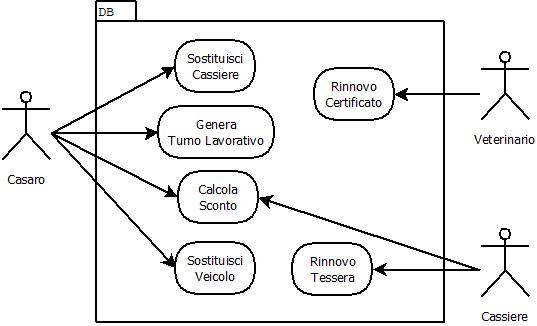
\includegraphics[scale=1]{imgs/UML/UML.jpeg}
\caption{Diagramma UML dei casi d'uso}
\end{figure}

\begin{itemize}
\item {Il Casaro ha il compito di sostituire un cassiere durante un turno lavorativo, da lui generato, mediante tale procedura. }

\begin{center}
 \begin{tabular}{l | r} 
 \textsc{Operazione} & SOSTITUISCI\_CASSIERE \\ [0.5ex] 
 \hline
 \textsc{Scopo} & sostituisce un cassiere durante un turno lavorativo. \\ 
 \textsc{Argomenti} & data e ora turno lavorativo, codice reparto. \\
 \textsc{Risultato} & sostituisce un cassiere affidato allo specifico turno\\
 \textsc{Errori}& NO\_DATA\_FOUND\\
 \textsc{Usa} & TurnoLavorativo, DipendenteCaseificio, Reparto\\ 
 \textsc{Modifica} & TurnoLavorativo \\ 
 \textsc{Prima} & è presente un cassiere che non può effettuare il turno per motivi personali\\ 
 \textsc{Poi} & il cassiere presente nel turno è stato sostituito da uno disponibile\\ [1ex] 
\end{tabular}
\end{center}

\item {Il Casaro ha il compito di gestire i Turni Lavorativi coinvolti. Tale procedura permette di gestire uno specifico turno lavorativo in base alle disponibilità del personale.  }

\begin{center}
 \begin{tabular}{l | r} 
 \textsc{Operazione} & GENERA\_TURNO\_LAVORATIVO \\ [0.5ex] 
 \hline
 \textsc{Scopo} & generare un turno lavorativo in base alla disponibilità del personale \\ 
 \textsc{Argomenti} & Data e Ora, Codice Reparto, Tesserino casaro responsabile. \\
 \textsc{Risultato} & aggiunta di un turno lavorativo\\
 \textsc{Errori}& NO\_DATA\_FOUND, addetti\_insufficienti, trasportatori\_insufficienti\\
 \textsc{Usa} & TurnoLavorativo, Reparto, assiste, consegna\\ 
 \textsc{Modifica} & TurnoLavorativo, Consegna, assiste\\ 
 \textsc{Prima} & non è presente un turno lavorativo in quella data per quel reparto\\ 
 \textsc{Poi} & è presente un turno lavorativo assegnato ai singoli dipendenti\\ [1ex] 
\end{tabular}
\end{center}

\item {Il Casaro ha il compito di sostituire un veicolo utilizzato durante un turno lavorativo. Potrebbe esser necessario sostituire il veicolo sulla base della disponibilità e del tipo di unità d'interesse per la raccolta del latte.}

\begin{center}
 \begin{tabular}{l | r} 
 \textsc{Operazione} & SOSTITUISCI\_VEICOLO \\ [0.5ex] 
 \hline
 \textsc{Scopo} & sostituire il veicolo sulla base del tipo di unità \\ 
 \textsc{Argomenti} & TipoUnita, Reparto, Data e Ora \\
 \textsc{Risultato} & sostituzione del veicolo in relazione a quello meno utilizzato e disponibile\\
 \textsc{Errori}& NO\_DATA\_FOUND\\
 \textsc{Usa} & si\_adopera, Veicolo, Reparto\\ 
 \textsc{Modifica} & si\_adopera\\ 
 \textsc{Prima} & è necessario sostituire un veicolo sulla base del tipo di unità\\ 
 \textsc{Poi} & è disponibile un veicolo per quel turno lavorativo\\ [1ex] 
\end{tabular}
\end{center}

\item {Il Casaro e il Cassiere, mediante questa procedura, hanno il compito di generare uno sconto sui prodotti mediante promozioni.}

\begin{center}
 \begin{tabular}{l | r} 
 \textsc{Operazione} & CALCOLA\_SCONTO \\ [0.5ex] 
 \hline
 \textsc{Scopo} & generare uno sconto basandosi sulla quantità dei prodotti in magazzino \\ 
 \textsc{Argomenti} & Coupon, DataScadenza, Sconto, EAN, NomeProdotto \\
 \textsc{Risultato} & aggiunta di uno sconto in relazione al prodotto desiderato\\
 \textsc{Errori}& NO\_DATA\_FOUND\\
 \textsc{Usa} & Prodotto, Promozione, utilizza\\ 
 \textsc{Modifica} & Promozione\\ 
 \textsc{Prima} & non è presente una promozione col codice inserito\\ 
 \textsc{Poi} & è presente una promozione col codice inserito\\ [1ex] 
\end{tabular}
\end{center}

\item {Il Cassiere ha il compito di effettuare il rinnovo delle tessere del Cliente, con eventuale modifica all'email associata. Ciò avviene mediante tale procedura. La tessera è normalmente rinnovata per un anno, ma può subire variazioni sulla base degli acquisti effettuati dal Cliente.}

\begin{center}
 \begin{tabular}{l | r} 
 \textsc{Operazione} & RINNOVO\_TESSERA \\ [0.5ex] 
 \hline
 \textsc{Scopo} & rinnovare la tessera del Cliente \\ 
 \textsc{Argomenti} & IDT, Email   \\
 \textsc{Risultato} & rinnovo della tessera sulla data di scadenza.\\
 \textsc{Errori}& NO\_DATA\_FOUND, tessera\_non\_scaduta\\
 \textsc{Usa} & Tessera, Cliente, utilizza  \\ 
 \textsc{Modifica} & Tessera\\ 
 \textsc{Prima} & la tessera interessata risulta scaduta\\ 
 \textsc{Poi} & la tessera interessata risulta rinnovata\\ [1ex] 
\end{tabular}
\end{center}

\item {Il Veterinario, mediante questa procedura, ha la possibilità di rinnovare i certificati di idoneità per animali interessati. Il rinnovo dei certificati può avvenire solo nelle seguenti modalità: se il Veterinario possiede un titolo di studio corrispondente alla Laurea Triennale, ha la possibilità di rinnovare i certificati dei solo Ovini; se il Veterinario possiede un titolo di studio corrispondente alla  Laurea  Magistrale,  ha  la  possibilità  di  rinnovare  i  certificati  di  tutti  gli  animali  coinvolti.Inoltre, risulta necessario rinnovare i certificati dei soli animali con data di emissione vecchia di almeno due anni.}

\begin{center}
 \begin{tabular}{l | r} 
 \textsc{Operazione} & RINNOVO\_CERTIFICATO \\ [0.5ex] 
 \hline
 \textsc{Scopo} & rinnova un certificato basandosi sull'idoneità di un animale\\ 
 \textsc{Argomenti} & NumCertificato, Idoneità, DataEmissione, CF\_Veterinario, EarTag \\
 \textsc{Risultato} & rinnovo di un certificato per l'animale\\
 \textsc{Errori}& NO\_DATA\_FOUND, vet\_non\_idoneo, cert\_ancora\_valido\\
 \textsc{Usa} & Veterinario, Animale, Certificato\\ 
 \textsc{Modifica} & Certificato\\ 
 \textsc{Prima} & è presente un certificato d'idoneità per l'animale da rinnovare\\ 
 \textsc{Poi} & è presente un certificato d'idoneità per l'animale\\ [1ex] 
\end{tabular}
\end{center}

\begin{center}
\begin{tabular}{ |c|c|c|c| }
	 \hline
 		\textbf{Operazione} & \textbf{Tipo} & \textbf{Volume} & \textbf{Periodo}\\
	 	\hline
 		SOSTITUISCI\_CASSIERE & B & 10 & Mese  \\ 
 		\hline
 		GENERA\_TURNO\_LAVORATIVO & B & 100 & Mese  \\ 
 		\hline
 		SOSTITUISCI\_VEICOLO & B & 20 & Mese  \\ 
 		\hline
 		CALCOLA\_SCONTO & B & 100 & Mese  \\ 
 		\hline
 		RINNOVO\_TESSERA & B & 50 & Mese  \\ 
 		\hline
 		RINNOVO\_CERTIFICATO & B & 20 & Mese  \\ 
 		\hline
 \end{tabular}\\
 \textit{Tipo: B (batch)}
\end{center}

\end{itemize}


\subsection{Diagrammi di sequenza UML}
Mediante i diagrammi di sequenza UML è possibile definire le interazioni tra i vari oggetti del nostro database nel corso del tempo. E' possibile fornire una visione dinamica del sistema mettendo alla luce il flusso di messaggi tra gli oggetti considerati e gli attori interessati. E' stato possibile definire i seguenti diagrammi di sequenza UML:

\begin{figure}[H]
\centering
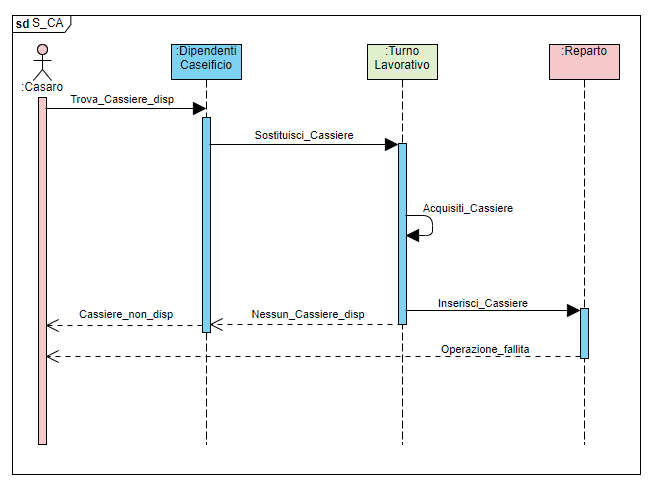
\includegraphics[scale=0.85]{imgs/UML/sdS_CA.PNG}
\caption{Diagramma di sequenza UML: SOSTITUISCI\_CASSIERE}
\end{figure}

\begin{figure}[H]
\centering
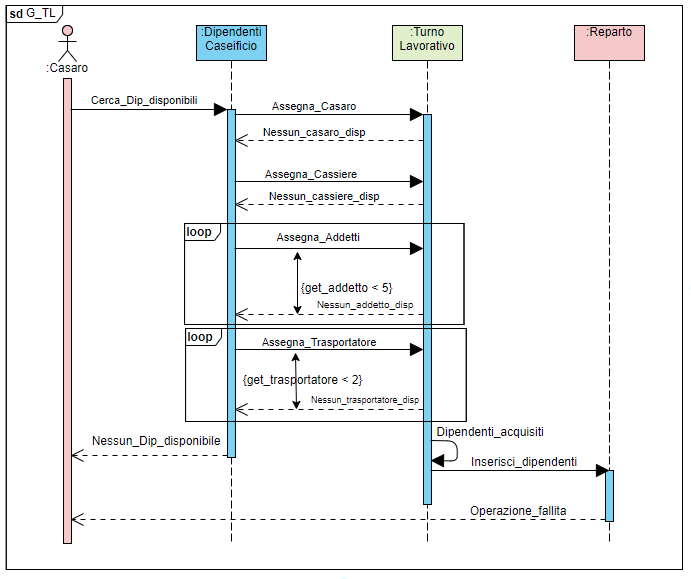
\includegraphics[scale=1]{imgs/UML/sdG_TL.PNG}
\caption{Diagramma di sequenza UML: GENERA\_TURNO\_LAVORATIVO}
\end{figure}

\begin{figure}[H]
\centering
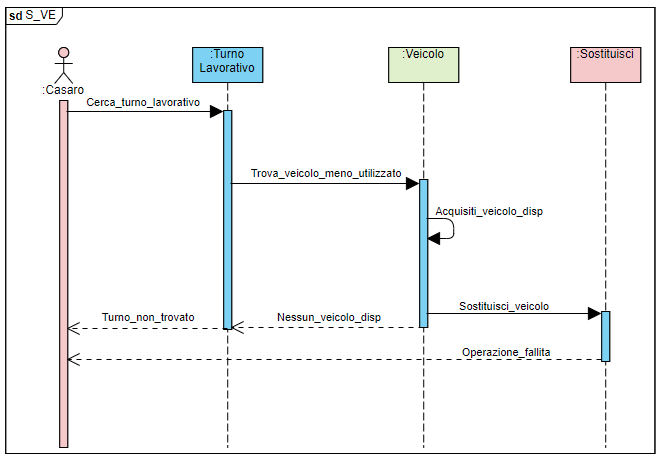
\includegraphics[scale=1]{imgs/UML/sdS_VE.PNG}
\caption{Diagramma di sequenza UML: SOSTITUISCI\_VEICOLO}
\end{figure}

\begin{figure}[H]
\centering
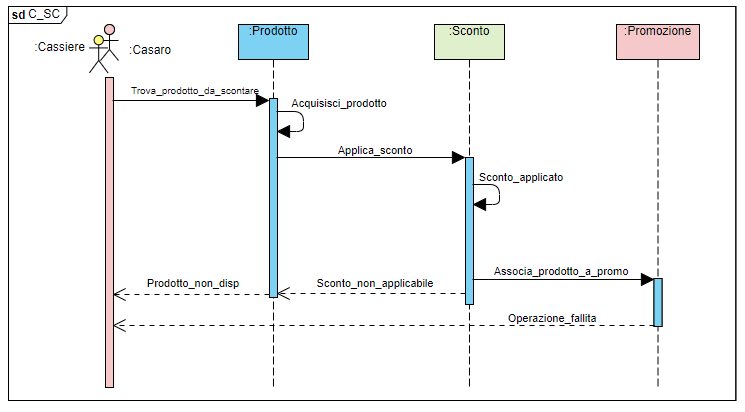
\includegraphics[scale=1]{imgs/UML/sdC_SC.PNG}
\caption{Diagramma di sequenza UML: CALCOLA\_SCONTO}
\end{figure}

\begin{figure}[H]
\centering
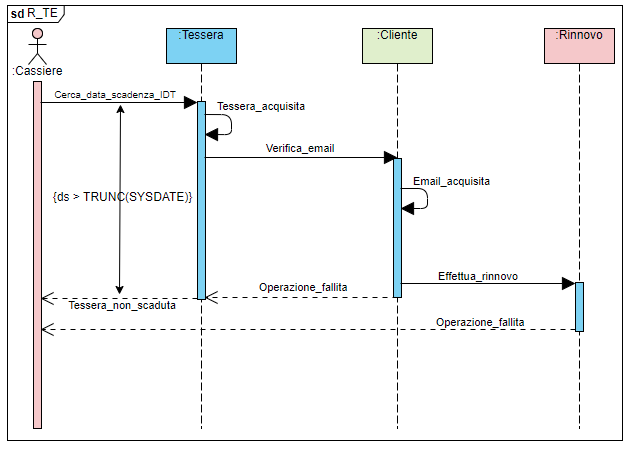
\includegraphics[scale=1]{imgs/UML/sdR_TE.PNG}
\caption{Diagramma di sequenza UML: RINNOVO\_TESSERA}
\end{figure}

\begin{figure}[H]
\centering
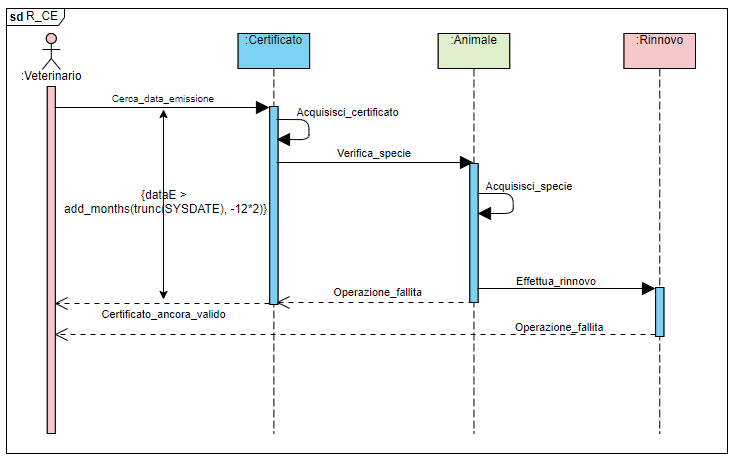
\includegraphics[scale=1]{imgs/UML/sdR_CE.PNG}
\caption{Diagramma di sequenza UML: RINNOVO\_CERTIFICATO}
\end{figure}

\section{Vincoli di integrità}
\subsection{Statici}
Di seguito è riportata un'analisi dei vincoli d'integrità statici più rilevanti presenti all'interno della base di dati. Sono tralasciati i vincoli d'integrità referenziale, unicità e di chiave primaria.
\begin{itemize}
\item \textbf{Persona}
	\begin{itemize}
	\item Il codice fiscale della persona deve essere valido. (Utilizzo di RegEx)
	\end{itemize}
\item \textbf{Cliente}
	\begin{itemize}
	\item L'email del cliente deve essere valida. (Utilizzo di RegEx)
	\end{itemize}
\item \textbf{Tessera}
	\begin{itemize}
	\item L'IDT della tessera deve essere valido. (Utilizzo di RegEx)
	\end{itemize}
\item \textbf{LabAnalisi}
	\begin{itemize}
	\item Il CUU del Laboratorio analisi deve essere valido. (Utilizzo di RegEx)
	\end{itemize}
\item \textbf{Promozione}
	\begin{itemize}
	\item Per politica interna e per offrire un tangibile vantaggio nell'utilizzo della carta, le promozioni devono offrire almeno il 10\% di sconto. (Utilizzo clausola CHECK)
	\item Il codice della promozione rispetta determinati standard. (Utilizzo di RegEx)
	\end{itemize}
\item \textbf{Prodotto}
	\begin{itemize}
	\item L'EAN del prodotto deve essere valido. (Utilizzo RegEx)
	\end{itemize}
\item \textbf{Veicolo}
	\begin{itemize}
	\item La targa del veicolo deve rispettare gli standard italiani. (Utilizzo RegEx)
	\end{itemize}
\item \textbf{Latte}
	\begin{itemize}
	\item Il bollino del latte deve essere valido. 
	\end{itemize}
	\item \textbf{Animale}
	\begin{itemize}
	\item Il codice dell'EarTag deve essere valido. 
	\end{itemize}
		\item \textbf{Certificato}
	\begin{itemize}
	\item Il certificato deve essere valido.
	\end{itemize}
	\item \textbf{Veterinario}
	\begin{itemize}
	\item Il titolo di studio del veterinario deve essere reale e valido. 
	\end{itemize}
	\item \textbf{Allevatore}
	\begin{itemize}
	\item La P.IVA dell'azienda allevatrice deve essere valida. (Utilizzo RegEx)
	\end{itemize}
	\item \textbf{DipendenteCaseificio}
	\begin{itemize}
	\item Il numero tesserino dei dipendenti deve essere valido.
	\end{itemize}
\item \textbf{Fattura}
	\begin{itemize}
	\item Il codice della fattura deve essere valido. (Utilizzo RegEx)
	\end{itemize}

\subsection*{Espressioni Regolari per la validazione dei campi}
Di seguito sono elencate l'insieme delle espressioni regolari utilizzare per validare i campi.
\begin{itemize}
\item \textbf{Codice Fiscale}: \begin{lstlisting}
  ^[A-Za-z]{6}[0-9]{2}[A-Za-z]{1}[0-9]{2}[A-Za-z]{1}[0-9]{3}[A-Za-z]{1}$
\end{lstlisting}
  Esempio campo valido: \textit{MDDLSS97D21F839P}\\
\item \textbf{Email}:\begin{lstlisting}
  ^[A-Za-z0-9._%-]+@[A-Za-z0-9.-]+[.][A-Za-z]+$
\end{lstlisting}
  Esempio campo valido: \textit{nome.cognome@email.it}\\ \\
\item \textbf{IDT}:\begin{lstlisting}
  ^[A-Z]{4}[0-9]{4}$
\end{lstlisting}
  Esempio campo valido: \textit{ABCD1234}\\
\item \textbf{CUU}:\begin{lstlisting}
  ^[0-9,A-Z]{6}$
\end{lstlisting}
  Esempio campo valido: \textit{A12BC3}\\
\item \textbf{FATTURA}:\begin{lstlisting}
  ^FA[0-9]{2}[A-Za-z]{3}$
\end{lstlisting}
  Esempio campo valido: \textit{FA12ABC}\\

\item \textbf{EAN}:\begin{lstlisting}
  ^[0-9]{8}$
\end{lstlisting}
  Esempio campo valido: \textit{648302200}\\
  \item \textbf{Coupon}:\begin{lstlisting}
  ^[0-9]{4}$
\end{lstlisting}
Esempio campo valido: \textit{3245}\\
\item \textbf{Targa}:\begin{lstlisting}
  ^[A-Za-z]{2}[0-9]{3}[A-Za-z]{2}$
\end{lstlisting}
  Esempio campo valido: \textit{BF764RD, bf764rd}\\
\item \textbf{P\_IVA}:\begin{lstlisting}
  ^[0-9]{11}
\end{lstlisting}
  Esempio campo valido: \textit{86334519757}\\
\end{itemize}

\end{itemize}
\subsection{Dinamici}

\begin{itemize}

\item \textbf{Persona} : per ragioni che concernono la responsabilità della società casearia, la tesserà sarà erogata solo a persone che hanno compiuto la maggiore età. Verrà effettuato un controllo sulla data di nascita.

\item \textbf{Tessera} : quando si tenta di aggiungere una nuova tessera nel DB, viene controllato che non sia presente una tessera già associata alla stessa persona (viene effettuato un controllo tramite codice fiscale). Qualora non esistesse un' altra tessera associata alla persona, viene applicata una politica di assegnazione della data di scadenza. Poichè è teoricamente un attributo in funzione di altri dati ottenibili tramite DB, dovrebbe in teoria rientrare nell'insieme di attributi derivati, tuttavia, trattandosi di operazioni potenzialmente onerose e dato che è un informazione a cui si fa spesso riferimento, si è deciso di memorizzarlo come attributo statico.
La politica di assegnazione della data di scadenza prende in considerazione la data di erogazione e imposta una validità della tessera in funzione di 1 anno solare.

Nel caso in cui la tessera è già presente nel database non può essere inserita. E' richiesta una procedura di rinnovo da parte di un Cassiere qualora la tessera sia inserita ma scaduta.
\item \textbf{Latte}: poichè il Latte è un alimento essenziale, risulta fondamentale effettuare dei controlli igienici-sanitari da parte di autorità competenti. L'analisi chimico-fisico è diretta ad accertare se l'alimento possieda i requisiti igienici e qualitativi previsti dalla legge "Disciplina del trattamento e della commercializzazione del latte alimentare vaccino 3 e 6 del regolamento CEE  n.
1411 del 29 giugno 1971" (fonte Gazzetta Ufficiale della Repubblica Italiana).
Tra le frodi ed alterazioni più comuni ritroviamo: l'innacquamento, scrematura, aggiunta di conservanti; mentre le sostanze nocive per il latte sono gli antibiotici e pesticidi. 

\item \textbf{Turno Lavorativo, Assiste, Consegna} Come precedente descritto nei requisiti la politica interna risulta piuttosto severa nei confronti del personale che partecipa ai turni. Per questo motivo è necessario che vi sia un casaro, un cassiere, addetti e trasportatori.

\item \textbf{ConsegnaCampione} E' compito del trasportatore prelevare campioni di latte per portarli a un Laboratorio Analisi affiliato all'attività per sottoporlo a esami di routine.
Il latte durante il trasporto deve essere conservato a una specifica temperatura e devono essere rispettate tutte le norme igienico-sanitarie.
Le analisi di routine prevedono: determinazione di grasso, proteine, lattosio, determinazione del sodio e potassio, determinazione della carica batterica, ricerca dei coliforni, ricerca degli antibiotici e titolazione dell'acido lattico.


\item \textbf{Utilizza} La tessera del Cliente rappresenta un metodo per invogliare l'acquisto. Con la sua sottoscrizione è possibile acquistare un prodotto in sconto del caseificio. L'utilizzo di questa tessera è in linea teorica per utilizzo personale/familiare. Gli utilizzi non sono accumulabili, la tessera NON è in alcun modo dotata di un sistema di punti fedeltà, di conseguenza non ci saranno ulteriori agevolazioni sui prodotti.
\end{itemize}


\section{Normalizzazione}

Valutare e quindi identificare a quale livello di normalizzazione lo schema si trova, è indispensabile per poterne valutare la qualità. Uno schema portato ad un livello \textit{k} di normalizzazione è sicuramente migliore - da un punto di vista qualitativo - di uno di livello \textit{k-1}, tuttavia ci sono ragioni per le quali il progettista decide di non portare un determinato schema ad una determinata forma normale. Le ragioni sono relative alla frammentazione dei dati e/o ragioni di performance (in particolare relative ai join necessari per ricostruire le informazioni).

\subsection*{Prima forma normale (1NF)}
Nella 1NF il dominio di ogni attributo deve comprendere solo valori atomici, il valore di ogni attributo delle tuple deve essere un valore singolo nel dominio dello stesso.
\newline\newline
Nel nostro contesto, se volessimo essere rigorosi, la prima forma normale non è rispettata per una serie di ragioni. Innanzitutto la presenza di numerosi attributi di tipo DATE (che in Oracle fanno riferimento sia ad un dato che vuole rappresentare una data che un orario). Inoltre è presente l'attributo "codice fiscale", il quale potrebbe essere visto come un agglomerato di informazioni tra cui la data di nascita che renderebbe l'attributo non conforme alla 1NF.
\newline\newline
Nel caso delle date, possiamo far riferimento al fatto che in numerosi contesti e linguaggi di programmazione, sia un dato considerato atomico. E' ugualmente possibile ritrovarci ad affrontare anomalie d'inserimento dettate dal fatto che l'identificazione della tupla (avendo utilizzato tale campo come chiave) si riduce ad una frazione di essa. Tuttavia il DBMS preclude tale possibilità (sebbene non in maniera definitiva) troncando l'attributo. I campi di contatto, in particolare quelli telefonici sono invece risolti da un punto di vista dello schema andando a creare una tabella per ognuno di essi. (es. telefono laboratorio, telefono dipendente o telefono persona). Attributi strutturati come quelli relativi all'indirizzo sono anch'essi risolti da un punto di vista dello schema andando a dividerli nelle loro singole componenti. Tale divisione però potrebbe dar origine ad anomalie di inserimento, modifica e cancellazione. Per poter escludere tali anomalie sarebbe necessario andare a fare controlli d'integrità locali relativi a tali attributi. (Ad esempio potrebbero essere inserite città con CAP errato: tuttavia un CAP potrebbe essere associato a più città. Per una corretta identificazione sarebbe corretto usare il codice ISTAT).
\newline\newline
A fronte di questo ragionamento e da scuole di pensiero, il considerare lo schema in prima forma normale o meno dipende dall'accezione di tali problematiche nei confronti dello schema.
\subsection*{Seconda forma normale (2NF)}
La 2NF implica che lo schema sia in 1NF. Se a fronte di quanto detto in precedenza volessimo considerare lo schema in prima forma normale, per ottenere la seconda forma normale è necessario che nelle relazioni che hanno come chiave un insieme di attributi, gli attributi primi che la compongono dipendano funzionalmente da tutte le chiavi e non da una parte di essa.
\newline\newline
Nel contesto del nostro schema, relazioni composte da tuple identificate univocamente da un gruppo di attributi sono numerose. Questo in particolare per le relazioni "TurnoLavorativo","Reparto", "DipendenteCaseificio"  entità deboli nel contesto dello schema EE/R. Tuttavia gli attributi di queste entità non dipendono funzionalmente da una parte della chiave. 
\newline\newline
Diverso è per quanto concerne le tabelle generate dalle relazioni M:N dello schema relativamente all'addetto per la tabella assiste e trasportatore per la tabella consegna. Qui c'è un vincolo d'integrità che ci impedisce di assegnare un dipendente a più di un turno lavorativo, ne consegue che il CF o il tesserino dipendono funzionalmente solo dalla data del turno lavorativo. Questo rende l'intero schema non in seconda forma normale.
\newline\newline
Sostituire la chiave del turno lavorativo, con un identificativo atomico, potrebbe in un certo senso risolvere tale problema, introducendo però una frammentazione dei dati e la necessità di verificare che non avvengano anomalie d'inserimento, modifica e cancellazione.
\newline\newline
Col desiderio di non introdurre chiavi artificiali di dubbia autorevolezza tale problema non è stato risolto.
\subsection*{Terza forma normale (3NF)}
La 3FN necessita che lo schema sia in seconda forma normale (non nel nostro contesto) e che non esistano attributi primi che dipendono da altri attributi primi. 
\newline\newline
Anche se il nostro schema fosse in 2FN, non avrebbe comunque i requisiti per soddisfare la 3FN in quanto sono presenti evidenti dipendenze funzionali per quanto riguarda gli attributi relativi ai luoghi (come ad esempio città e provincia). Correggere tali attributi richiederebbe un'ulteriore frammentazione dei dati anche per accedere a "semplici" dati come un indirizzo. Questo causerebbe inevitabilmente una perdita di prestazioni per ogni tipologia di operazioni su questo database.
\newline\newline
Questo ne consegue, per ovvie ragioni, l'impossibilità di raggiungere la forma Normale di Boyce \& Codd.

\section{Volumi e prestazioni attese}
Trattandosi di una database in scala regionale, l'insieme dei possibili accessi dipende dalla mole di turni lavorativi e di acquisti effettuati. Analizzando il caso reale, la presenza dei veicoli risulta essere di circa 10 unità al giorno. Tale organizzazione produce un modesto traffico di informazioni. Popolare l'intero DB con dati fittizi risulta essere particolarmente ostico, in quanto non solo interviene la variazione di vendite effettuate ma incombono una serie di influenze dettate dal mercato e dall'esigenza di chi magari utilizza la tessera. Pertanto, i dati inseriti per popolare inizialmente il DB sono innanzitutto limitati alla regione Campania. Prendendo in considerazione le tabelle, e tenendo conto che è solo un'operazione didattica, in quanto la reale mole di informazioni potrebbe esponenzialmente crescere, i volumi iniziali delle tabelle sono i seguenti:

\begin{center}
 \begin{tabular}{||l c c c c||} 
 \hline
 Tabella & Tipo & Volume & Incremento & Periodo \\ [0.5ex] 
 \hline\hline
    Persona & E & 40 & 50+ & mese \\
    CellularePersona & E & 40 & 50+ & mese \\
    Cliente & E & 30 & 50+ & mese \\
    Veterinario & E & 10 & 50 & mese \\
    Tessera & E & 30 & 100 & anno \\
    utilizza & A & 40 & 80+ & mese \\
    Promozione & E & 40 & 100+ & mese \\
    Prodotto & E & 40 & 70+ & mese \\
    Carrello & E & 40 & 100 & mese \\
    e\_parte & A & 40 & 50 & mese \\
    Fattura & E & 40 & 100+ & mese \\
    acquista & A & 40 & 100+ & mese \\
    Certificato & E & 30 & 50 & mese \\
    Animale & E & 40 & 70 & mese \\
    produce & A & 50 & 40+ & mese \\
    Allevatore & E & 40 & 70 & mese \\
    Latte & E & 40 & 80+ & mese \\
    DipendenteCaseificio & E & 20 & 30+ & anno \\
    CellulareDipendente & E & 20 & 30+ & mese \\
    assiste & A & 30 & 10 & mese\\
    consegna & A & 20 & 10 & mese\\
    TurnoLavorativo & ED & 50 & 200 & mese \\
    Veicolo & E & 10 & 15+ & anno \\
    si\_adopera & A & 20 & 10 & mese \\
    Reparto & E & 40 & 100+ & mese \\
    LabAnalisi & E & 50 & 50 & mese \\
    TelefonoLab & E & 50 & 50 & mese \\
    ConsegnaCampione & E & 60 & 70+ & mese \\
    Referto & E & 60 & 70+ & mese \\
    Esame & E & 20 & 5 & mese \\
    e\_composta\_da & A & 60 & 40+ & mese \\     
 
 \hline
\end{tabular}\\
\textit{Tipo: E - entità, ED - entità debole, A - associazione}
\end{center}

\newpage

\section{Estensioni}
Le estensioni possibili a questo progetto sono innumerevoli. Trattandosi di un progetto a scopo di didattico si potrebbe pensare di estendere lo schema relazionale in modo da gestire in maniera più precisa e corretta i dati relativi ai referti ed ai singoli esami.\\\\
La gestione delle promozioni potrebbe essere rivisitata andando a selezionare e generare automaticamente delle promozioni in base ai dati di vendita dei singoli prodotti (e quindi avere accesso ai dati delle vendite).\\\\
Come scheduler programmati temporalmente si potrebbe pensare di attivare promozioni in base al periodo dell'anno (es: attivare sconti per tutti i prodotti di stagione).\\\\
Si potrebbe inoltre creare un sistema automatico relativo ai posti disponibili nel parcheggio aziendale.\\\\
Sarà possibile estendere il concetto di cliente in locali e grossisti considerando spedizioni estere.\\\\
Un importante upgrade del DB potrebbe essere la gestione delle autorizzazioni sanitarie sugli animali adibiti alla produzione di latte.\\\\
\chapter{Implementazione}
\section*{Premessa}
Facendo uso del tipo DATE di Oracle, il mese delle date è scritto in lingua italiana. Qualora non si voglia impostare globalmente la lingua italiana del DBMS, è sufficiente modificare la lingua della sessione con il seguente comando:

\begin{lstlisting}
	ALTER SESSION SET NLS_DATE_LANGUAGE = 'ITALIAN';
\end{lstlisting}
Inoltre , qualora si voglia visualizzare correttamente i dati presenti e le tabelle facendo uso di client come sqlplus e quindi da linea di comando, è consigliabile modificare il numero di colonne visualizzabili da terminale.

\begin{lstlisting}
	set linesize 300
\end{lstlisting}
Dove 300 è il numero di colonne di caratteri visualizzabili da terminale. È possibile cambiare tale valore in funzione del contenuto che si visualizza.
\begin{lstlisting}
    alter session set "_ORACLE_SCRIPT"=true;  
\end{lstlisting}
Questa istruzione modifica la sessione e permette la creazione degli utenti.


\section{Creazione Utenti}
La prima operazione da effettuare per poter mettere in piedi il nostro database è la creazione degli utenti. Per farlo è sufficiente accedere al DBMS come amministratore di sistema e lanciare il relativo script per la creazione degli utenti:

\begin{lstlisting}[language=SQL,caption={CREA\_UTENTI}]
	CREATE USER Caseificio IDENTIFIED BY 123;
	GRANT ALL PRIVILEGES TO Caseificio;
	CREATE USER Casaro IDENTIFIED BY 123;
	CREATE USER Cassiere IDENTIFIED BY 123;
	CREATE USER Addetto IDENTIFIED BY 123;
	CREATE USER Trasportatore IDENTIFIED BY 123;
	CREATE USER Allevatore IDENTIFIED BY 123;
	CREATE USER Cliente IDENTIFIED BY 123;
	CREATE USER Analista IDENTIFIED BY 123;
	CREATE USER Veterinario IDENTIFIED BY 123;
\end{lstlisting}
In questo caso vengono impostate delle password fittizie (123) per tutti gli utenti. In particolare l'utente Caseificio sarà amministratore dell'intero DBMS (Prestare attenzione nel caso in cui siano presenti più basi di dati). Nel caso in cui sia già stato fatto un tentativo di esecuzione e/o siano presenti utenti omonimi nel DBMS è necessario prima di creare utenti, di cancellare quelli già presenti:
\begin{lstlisting}[language=SQL,caption={DROP\_UTENTI}]
	DROP USER Caseificio CASCADE;
	DROP USER Casaro;
	DROP USER Cassiere;
	DROP USER Addetto;
	DROP USER Trasportatore;
	DROP USER Allevatore;
	DROP USER Cliente;
	DROP USER Analista;
	DROP USER Veterinario;
\end{lstlisting}
Dopo la creazione degli utenti, è possibile (e consigliabile) accedere come utente Caseificio che nel nostro contesto rappresenta l'amministratore del DB.

\section{Creazione tabelle}
Seguendo lo schema relazionale è possibile tramutare le tabelle presenti nello schema in vere e proprie tabelle della nostra base di dati tramite l'istruzione CREATE. Sono inoltre definiti nelle CREATE stesse anche i vincoli di chiave primaria, d'integrità referenziale e vincoli d'integrità statici. Per poter rispettare i vincoli d'integrità referenziale è necessario creare le tabelle dando precedenza a quelle che non fanno riferimento ad alcuna chiave esterna, procedendo a ritroso seguendo lo schema relazionale. Prima di procedere è necessario però cancellare tramite comando DROP le tabelle precedentemente create (rispettando un certo ordine):

\begin{lstlisting}[language=SQL,caption={DROP\_TABELLE}]
    DROP TABLE e_composta_da;
    DROP TABLE Fattura;
    DROP TABLE Referto;
    DROP TABLE ConsegnaCampione;
    DROP TABLE Esame;
    DROP TABLE TelefonoLab;
    DROP TABLE LabAnalisi;
    DROP TABLE si_adopera;
    DROP TABLE consegna;
    DROP TABLE assiste;
    DROP TABLE produce;
    DROP TABLE Latte;
    DROP TABLE TurnoLavorativo;
    DROP TABLE Veicolo;
    DROP TABLE Reparto;
    DROP TABLE CellulareDipendente;
    DROP TABLE DipendenteCaseificio;
    DROP TABLE Animale;
    DROP TABLE Allevatore;
    DROP TABLE Certificato;
    DROP TABLE acquista;
    DROP TABLE e_parte;
    DROP TABLE utilizza;
    DROP TABLE Promozione;
    DROP TABLE Prodotto;    
    DROP TABLE Carrello; 
    DROP TABLE Veterinario;
    DROP TABLE Tessera;
    DROP TABLE Cliente;
    DROP TABLE CellularePersona;
    DROP TABLE Persona;
\end{lstlisting}

\subsection*{Persona}
\begin{lstlisting}[language=SQL,caption={CREA\_TABELLE}]
    CREATE TABLE Persona(
        CF CHAR(16) NOT NULL, 
        NomeP VARCHAR(30) NOT NULL,
        CognomeP VARCHAR(30) NOT NULL,
        DataNascitaP DATE NOT NULL,
        CONSTRAINT PK_PERSONA PRIMARY KEY (CF),
        CONSTRAINT CF_NOTVALID CHECK (REGEXP_LIKE (CF, '^[A-Za-z]{6}[0-9]{2}[A-Za-z]{1}[0-9]{2}[A-Za-z]{1}[0-9]{3}[A-Za-z]{1}$'))
    );
\end{lstlisting}

\subsection*{CellularePersona}
\begin{lstlisting}[language=SQL]
    CREATE TABLE CellularePersona(
        CF CHAR(16) NOT NULL,
        Cellulare VARCHAR(10),
        CONSTRAINT FK_CellulareP FOREIGN KEY (CF) REFERENCES Persona(CF),
        CONSTRAINT CELL_NOTVALID_PERSONA CHECK (LENGTH(Cellulare) >= 9 AND 
        LENGTH (Cellulare) <= 11)
    );   
\end{lstlisting}

\subsection*{Cliente}
\begin{lstlisting}[language=SQL]
    CREATE TABLE Cliente(
        ClienteCF  CHAR(16) NOT NULL,
        Email VARCHAR(30),
        CONSTRAINT PK_CLIENTE PRIMARY KEY (ClienteCF),
        CONSTRAINT FK_CLIENTE FOREIGN KEY (ClienteCF) REFERENCES Persona(CF),
        CONSTRAINT EMAIL_NOTVALID CHECK (REGEXP_LIKE     (Email,'^[A-Za-z0-9._%-]+@[A-Za-z0-9.-]+[.][A-Za-z]+$'))
    );
\end{lstlisting}

\subsection*{Tessera}
\begin{lstlisting}[language=SQL]
    CREATE TABLE Tessera(
        IDT CHAR(8) NOT NULL,
        DataScadenza DATE,
        CF_Cliente CHAR(16) NOT NULL, 
        DataErogazione DATE NOT NULL,
        CONSTRAINT PK_TESSERA PRIMARY KEY (IDT),
        CONSTRAINT FK_TESSERA FOREIGN KEY (CF_Cliente) REFERENCES Cliente(ClienteCF),
        CONSTRAINT IDT_NOTVALID CHECK (REGEXP_LIKE(IDT,'^[A-Z]{4}[0-9]{4}$'))
    );
\end{lstlisting}

\subsection*{Veterinario}
\begin{lstlisting}[language=SQL]
    CREATE TABLE Veterinario(
        VeterinarioCF CHAR(16) NOT NULL,
        TitoloDiStudio VARCHAR(30),
        CONSTRAINT PK_VETERINARIO PRIMARY KEY (VeterinarioCF),
        CONSTRAINT FK_VETERINARIO FOREIGN KEY (VeterinarioCF) REFERENCES Persona(CF)
    );
\end{lstlisting}

\subsection*{Carrello}\begin{lstlisting}[language=SQL]
    CREATE TABLE Carrello (
        Doc_N CHAR(9) NOT NULL,
        Quantita NUMBER,
        CONSTRAINT PK_CARRELLO PRIMARY KEY (Doc_N)
    );   
\end{lstlisting}

\subsection*{Prodotto}\begin{lstlisting}[language=SQL]
    CREATE TABLE Prodotto(
        EAN CHAR(8) NOT NULL,
        NomeProdotto VARCHAR(40) NOT NULL,
        Prezzo NUMBER NOT NULL,
        CONSTRAINT PK_PRODOTTO PRIMARY KEY (EAN),
        CONSTRAINT EAN_NOTVALID CHECK (REGEXP_LIKE (EAN,'^[0-9]{8}$'))
    );
\end{lstlisting}

\subsection*{Promozione}
\begin{lstlisting}[language=SQL]
    CREATE TABLE Promozione(
        Coupon CHAR(4) NOT NULL,
        DataScadenzaP DATE NOT NULL,
        Sconto NUMBER NOT NULL,
        CodEANProd CHAR(8),
        CONSTRAINT PK_COUPON PRIMARY KEY (Coupon),
        CONSTRAINT SCONTO_PROMOZIONE CHECK (Sconto >= 10),
        CONSTRAINT COUPON_NOTVALID CHECK (REGEXP_LIKE (Coupon,'^[0-9]{4}$')),
        CONSTRAINT FK_PROMOZIONE FOREIGN KEY (CodEANProd) REFERENCES Prodotto(EAN)
    );
\end{lstlisting}

\newpage

\subsection*{utilizza}\begin{lstlisting}[language=SQL]
    CREATE TABLE utilizza(
		IDT_Tessera CHAR(8) NOT NULL,
		DataUtilizzo DATE NOT NULL,
		CodCoupon CHAR(4) NOT NULL,
		CONSTRAINT FK1_UTILIZZA FOREIGN KEY (IDT_Tessera) REFERENCES Tessera(IDT),
		CONSTRAINT FK2_UTILIZZA FOREIGN KEY (CodCoupon) REFERENCES Promozione(Coupon)
	);
\end{lstlisting}

\subsection*{e\_parte}\begin{lstlisting}[language=SQL]
    CREATE TABLE e_parte(
		ProdottoEAN CHAR(8),
		NumeroDoc CHAR(9),
		CONSTRAINT FK1_E_PARTE FOREIGN KEY (ProdottoEAN) REFERENCES Prodotto(EAN),
		CONSTRAINT FK2_E_PARTE FOREIGN KEY (NumeroDoc) REFERENCES Carrello(Doc_N)
	);
\end{lstlisting}

\subsection*{acquista}\begin{lstlisting}[language=SQL]
    CREATE TABLE acquista(
        CodiceFiscaleP CHAR(16) NOT NULL,
        NumeroDocumento CHAR(9) NOT NULL, 
        CONSTRAINT FK1_ACQUISTA FOREIGN KEY (CodiceFiscaleP) REFERENCES Persona(CF),
        CONSTRAINT FK2_ACQUISTA FOREIGN KEY (NumeroDocumento) REFERENCES Carrello(Doc_N)
    );
\end{lstlisting}

\subsection*{Certificato}\begin{lstlisting}[language=SQL]
    CREATE TABLE Certificato(
        NumCertificato CHAR(6) NOT NULL,
        Idoneita CHAR(1)  not null,
        DataEmissione   DATE not null,
        CF_Veterinario Char(16) not null,
        CONSTRAINT  PK_CERTIFICATO PRIMARY KEY (NumCertificato),
        CONSTRAINT  FK_CERTIFICATO FOREIGN KEY (CF_Veterinario) REFERENCES
        Veterinario(VeterinarioCF),
        CONSTRAINT  IDO_NOTVALID  CHECK (Idoneita IN ('T','F'))
    );
\end{lstlisting}

\subsection*{Allevatore}\begin{lstlisting}[language=SQL]
    CREATE TABLE Allevatore(
        P_IVA CHAR(11) NOT NULL,
        NomeAllevamento VARCHAR(30) NOT NULL,
        MqTerreno NUMBER,
        ModAllevamento VARCHAR(30) NOT NULL,
        Via VARCHAR(30),
        Cap CHAR(5) NOT NULL,
        Citta VARCHAR(30) NOT NULL,
        CONSTRAINT PK_ALLEVATORE PRIMARY KEY (P_IVA),
        CHECK (( ModAllevamento = 'Intensivo') OR (ModAllevamento = 'Estensivo')),
        CONSTRAINT PIVA_NOTVALID CHECK (REGEXP_LIKE ( P_IVA,'^[0-9]{11}'))
    );
\end{lstlisting}

\subsection*{Animale}\begin{lstlisting}[language=SQL]
	CREATE TABLE Animale(
        EarTag CHAR(6) NOT NULL,
        Specie VARCHAR(30) NOT NULL,
        DataNascita DATE,
        Peso NUMBER,
        PartitaIVA CHAR(11) NOT NULL,
        CertificatoA CHAR(6) NOT NULL,
        CHECK (Specie IN ('Bovino','Caprino','Ovino')),
        CONSTRAINT PK_ANIMALE PRIMARY KEY (EarTag),
        CONSTRAINT FK1_ANIMALE FOREIGN KEY (PartitaIVA) REFERENCES Allevatore(P_IVA),
        CONSTRAINT FK2_ANIMALE FOREIGN KEY (CertificatoA) REFERENCES Certificato(NumCertificato)
    );
\end{lstlisting}

\subsection*{DipendenteCaseificio}
\begin{lstlisting}[language=SQL]
    CREATE TABLE DipendenteCaseificio(
        NumTesserino CHAR(5) NOT NULL,
        NomeD VARCHAR(30) NOT NULL,
        CognomeD VARCHAR(30) NOT NULL,
        DataNascitaD DATE NOT NULL,
        OreLavorative NUMBER NOT NULL,
        CostoOrario NUMBER,
        Ruolo VARCHAR(20) NOT NULL,
        CONSTRAINT PK_DIPENDENTE PRIMARY KEY (NumTesserino),
        CONSTRAINT RUOLO_DIPENDENTE CHECK (Ruolo IN ('Cassiere','Casaro','Addetto',
        'Trasportatore'))
    );
\end{lstlisting}

\subsection*{CellulareDipendente}
\begin{lstlisting}[language=SQL]
    CREATE TABLE CellulareDipendente(
        Tesserino CHAR(5) NOT NULL,
        Cellulare VARCHAR(10) NOT NULL,
        CONSTRAINT FK_CELL_DIPENDENTE FOREIGN KEY (Tesserino) REFERENCES 
        DipendenteCaseificio(NumTesserino),
        CONSTRAINT CELL_NOTVALID_DIPENDENTE CHECK (LENGTH(Cellulare) >= 9 AND 
        LENGTH (Cellulare) <= 11)
    );   
\end{lstlisting}

\newpage

\subsection*{Reparto}
\begin{lstlisting}[language=SQL]
    CREATE TABLE Reparto(
        CodR CHAR(5) NOT NULL,
        NomeR VARCHAR(30) NOT NULL,
        CapienzaR NUMBER,
        CONSTRAINT PK_REPARTO PRIMARY KEY (CodR),
        CHECK (CapienzaR <= 10)
    );
\end{lstlisting}

\subsection*{Veicolo}
\begin{lstlisting}[language=SQL]
    CREATE TABLE Veicolo(
        Targa CHAR(7) NOT NULL,
        CapienzaV NUMBER,
        TipoUnita VARCHAR(20) NOT NULL,
        CONSTRAINT PK_VEICOLO PRIMARY KEY (Targa),
        CHECK (TipoUnita IN ('Autocarro', 'Cisterna', 'Rimorchio', 'Scarrabile')),
        CONSTRAINT TARGA_NOTVALID CHECK (REGEXP_LIKE (Targa,'^[A-Za-z]{2}[0-9]{3}[A-Za-z]{2}$'))
    );
\end{lstlisting}

\subsection*{TurnoLavorativo}
\begin{lstlisting}[language=SQL]
    CREATE TABLE TurnoLavorativo(
        Data_Ora DATE NOT NULL,
        CodiceReparto CHAR(5) NOT NULL,
        CassiereTess CHAR(5) NOT NULL,
        CasaroTess CHAR(5) NOT NULL,
        CONSTRAINT PK_TurnoL PRIMARY KEY (Data_Ora, CodiceReparto),
        CONSTRAINT FK1_TurnoL FOREIGN KEY (CodiceReparto) REFERENCES Reparto(CodR),
        CONSTRAINT FK2_TurnoL FOREIGN KEY (CassiereTess) REFERENCES 
        DipendenteCaseificio(NumTesserino),
        CONSTRAINT FK3_TurnoL FOREIGN KEY (CasaroTess) REFERENCES 
        DipendenteCaseificio (NumTesserino)
    );
\end{lstlisting}

\subsection*{Latte}\begin{lstlisting}[language=SQL]
    CREATE TABLE Latte(
        NumBollino CHAR(7) NOT NULL,
        DataProduzione DATE NOT NULL,
        DataScadenza DATE NOT NULL,
        Tipologia VARCHAR(30) NOT NULL,
        QuantitaL NUMBER NOT NULL,
        TempConservazione VARCHAR(30),
        Data_OraTL DATE NOT NULL,
        CodRepartoTL CHAR(5) NOT NULL,
        CONSTRAINT PK_LATTE PRIMARY KEY (NumBollino),
        CONSTRAINT FK_LATTE FOREIGN KEY (Data_OraTL, CodRepartoTL) REFERENCES TurnoLavorativo(Data_Ora, CodiceReparto)
    );
\end{lstlisting}

\subsection*{produce}\begin{lstlisting}[language=SQL]
   CREATE TABLE produce(
        CodiceEarTag CHAR(6) NOT NULL,
        NumeroBollino CHAR(7) NOT NULL,
        CONSTRAINT FK1_PRODUCE FOREIGN KEY (CodiceEarTag) REFERENCES Animale (EarTag),
        CONSTRAINT FK2_PRODUCE FOREIGN KEY (NumeroBollino) REFERENCES Latte (NumBollino)
    );
\end{lstlisting}

\subsection*{assiste}
\begin{lstlisting}[language=SQL]
    CREATE TABLE assiste(
        AddettoTess CHAR(5) NOT NULL,
        CodiceRep CHAR(5) NOT NULL,
        DataOraTL DATE NOT NULL,
        CONSTRAINT FK1_ASSISTE FOREIGN KEY (AddettoTess) REFERENCES 
        DipendenteCaseificio(NumTesserino),
        CONSTRAINT FK2_ASSISTE FOREIGN KEY (CodiceRep) REFERENCES Reparto(CodR),
        CONSTRAINT FK3_ASSISTE FOREIGN KEY (DataORATL, CodiceRep) REFERENCES 
        TurnoLavorativo(Data_Ora,CodiceReparto)
    );
\end{lstlisting}

\subsection*{consegna}
\begin{lstlisting}[language=SQL]
    CREATE TABLE consegna(
        TrasportatoreTess CHAR(5) NOT NULL,
        CodiceRep CHAR(5) NOT NULL,
        DataOraTL DATE NOT NULL,
        CONSTRAINT FK1_CONSEGNA FOREIGN KEY (TrasportatoreTess) REFERENCES 
        DipendenteCaseificio(NumTesserino),
        CONSTRAINT FK2_CONSEGNA FOREIGN KEY (CodiceRep) REFERENCES Reparto(CodR),
        CONSTRAINT FK3_CONSEGNA FOREIGN KEY (DataOraTL, CodiceRep) REFERENCES
        TurnoLavorativo(Data_Ora,CodiceReparto)
    );
\end{lstlisting}

\subsection*{si\_adopera}
\begin{lstlisting}[language=SQL]
    CREATE TABLE si_adopera(
        Targa CHAR(7) NOT NULL,
        CodReparto CHAR(5) NOT NULL,
        Data_Ora_TL DATE NOT NULL,
        CONSTRAINT FK1_SI_ADOPERA FOREIGN KEY (Targa) REFERENCES Veicolo(Targa),
        CONSTRAINT FK2_SI_ADOPERA  FOREIGN KEY (CodReparto) REFERENCES Reparto(CodR),
        CONSTRAINT FK3_SI_ADOPERA  FOREIGN KEY (Data_Ora_TL, CodReparto) REFERENCES
        TurnoLavorativo(Data_Ora,CodiceReparto)
    );
\end{lstlisting}

\newpage

\subsection*{LabAnalisi}
\begin{lstlisting}[language=SQL]
    CREATE TABLE LabAnalisi(
        CUU	CHAR(6)	NOT NULL, 
        NomeLab	VARCHAR(20)	NOT NULL, 
        Via VARCHAR(30), 
        Cap CHAR(5) NOT NULL, 
        Citta  VARCHAR(30) NOT NULL,
        CONSTRAINT PK_LAB_ANALISI PRIMARY KEY (CUU),
        CONSTRAINT CUU_NOTVALID CHECK (REGEXP_LIKE (CUU,'^[0-9,A-Z]{6}$'))
    );
\end{lstlisting}

\subsection*{TelefonoLab}
\begin{lstlisting}[language=SQL]
    CREATE TABLE TelefonoLab(
        CUU_Lab	char(6)	NOT NULL, 
        Telefono VARCHAR(10) NOT NULL, 
        CONSTRAINT FK_LAB_ANALISI FOREIGN KEY (CUU_LAB) REFERENCES LabAnalisi (CUU),
        CONSTRAINT TEL_NOTVALID_LAB CHECK (LENGTH(Telefono) >=9 AND 
        LENGTH(Telefono) <=11)
    );
\end{lstlisting}

\subsection*{Esame}
\begin{lstlisting}[language=SQL]
    CREATE TABLE Esame(
		CodMnemonico CHAR(5) NOT NULL,
		NomeEsame VARCHAR(30) NOT NULL,
		CONSTRAINT PK_ESAME PRIMARY KEY (CodMnemonico)
    );
\end{lstlisting}

\subsection*{ConsegnaCampione}
\begin{lstlisting}[language=SQL]
    CREATE TABLE ConsegnaCampione(
		CodCamp CHAR(5) NOT NULL,
		Data_OraConsegna DATE NOT NULL,
		Data_Ora DATE NOT NULL,
		CodiceRepartoTL CHAR(5) NOT NULL,
		CONSTRAINT PK_CONSEGNA_CAMPIONE PRIMARY KEY (CodCamp),
		CONSTRAINT FK_CONSEGNA_CAMPIONE FOREIGN KEY (Data_Ora, CodiceRepartoTL) REFERENCES 
		TurnoLavorativo (Data_Ora, CodiceReparto)
    );
\end{lstlisting}

\newpage

\subsection*{Referto}
\begin{lstlisting}[language=SQL]
    CREATE TABLE Referto(
	    CodPrestazione CHAR(8) NOT NULL,
	    NomeAnalista VARCHAR(30),
	    CognomeAnalista VARCHAR(30),
	    CUU_LabA CHAR(6),
	    CodCampione CHAR(5),
	    CONSTRAINT PK_REFERTO PRIMARY KEY (CodPrestazione),
	    CONSTRAINT FK1_REFERTO FOREIGN KEY (CUU_LabA) REFERENCES 
	    LabAnalisi(CUU),
	    CONSTRAINT FK2_REFERTO FOREIGN KEY (CodCampione) REFERENCES
	    ConsegnaCampione(CodCamp)
    );
\end{lstlisting}

\subsection*{Fattura}
\begin{lstlisting}[language=SQL]
     CREATE TABLE Fattura(
	   CodFattura CHAR(7) NOT NULL,
	   Importo NUMBER NOT NULL,
	   DataTurnoLavorativo DATE,
	   Codice_Reparto CHAR(5),
	   Num_Doc CHAR(9),
	   CodiceFiscalePersona CHAR(16),
	   CONSTRAINT PK_FATTURA PRIMARY KEY (CodFattura),
	   CONSTRAINT FK1_FATT FOREIGN KEY (DataTurnoLavorativo,Codice_Reparto) REFERENCES
	   TurnoLavorativo(Data_Ora,CodiceReparto),
	   CONSTRAINT FK2_FATT FOREIGN KEY (Num_Doc) REFERENCES Carrello(Doc_N),
	   CONSTRAINT FK3_FATT FOREIGN KEY (CodiceFiscalePersona) REFERENCES Persona(CF),
	   CONSTRAINT FATTURA_NOTVALID CHECK (REGEXP_LIKE (CodFattura,'^FA[0-9]{2}[A-Za-z]{3}$'))
    );
\end{lstlisting}

\subsection*{e\_composta\_da}
\begin{lstlisting}[language=SQL]
    CREATE TABLE e_composta_da(
	   CodicePrestazione CHAR(8) NOT NULL,
	   CodiceMnemonico CHAR(5) NOT NULL,
	   ValEsito NUMBER NOT NULL,
	   Giudizio CHAR(3) NOT NULL,
	   CONSTRAINT FK1_COMP FOREIGN KEY (CodicePrestazione) REFERENCES
	   Referto(CodPrestazione),
	   CONSTRAINT FK2_COMP FOREIGN KEY (CodiceMnemonico) REFERENCES
	   Esame(CodMnemonico),
	   CONSTRAINT COMP_NOTVALID CHECK (Giudizio IN ('pos','neg'))
    );
\end{lstlisting}

\newpage

\section{Gestione permessi utente}
Dopo aver creato le tabelle del nostro database e aver ad disposizione l'insieme degli utenti che ne usufruiranno è necessario andare ad implementare i permessi di lettura, scrittura e visualizzazione seguendo quanto indicato nel capitolo precedente.

\begin{lstlisting}[language=SQL,caption={DCL\_UTENTI}]
	-- Casaro
	GRANT SELECT ON DipendenteCaseificio TO Casaro;
	GRANT ALL PRIVILEGES ON CellulareDipendente TO Casaro;
	GRANT ALL PRIVILEGES ON TurnoLavorativo TO Casaro;
	GRANT ALL PRIVILEGES ON Reparto TO Casaro;
	GRANT ALL PRIVILEGES ON Veicolo TO Casaro;
	GRANT ALL PRIVILEGES ON ConsegnaCampione TO Casaro;
	GRANT SELECT  ON LabAnalisi TO Casaro;
	GRANT SELECT  ON TelefonoLab  TO Casaro;
        GRANT SELECT ON Referto TO Casaro;
        GRANT SELECT ON e_composta_da  TO Casaro;
        GRANT SELECT ON Esame TO Casaro;
        GRANT ALL PRIVILEGES ON Latte TO Casaro;
        GRANT ALL PRIVILEGES ON Promozione TO Casaro;
        GRANT ALL PRIVILEGES ON Prodotto TO Casaro;
        GRANT SELECT ON Persona TO Casaro;
        GRANT SELECT ON CellularePersona TO Casaro;
        GRANT SELECT ON Allevatore TO Casaro;
        GRANT SELECT ON Animale TO Casaro;
        GRANT SELECT ON Certificato TO Casaro;
        GRANT SELECT ON Veterinario TO Casaro;
	
	-- Cassiere
	GRANT SELECT ON DipendenteCaseificio TO Cassiere;
	GRANT ALL PRIVILEGES ON CellulareDipendente TO Cassiere;
	GRANT SELECT ON TurnoLavorativo TO Cassiere;
	GRANT SELECT ON Reparto TO Cassiere;
	GRANT SELECT ON Persona TO Cassiere;
	GRANT SELECT ON CellularePersona TO Cassiere;
	GRANT ALL PRIVILEGES ON Cliente TO Cassiere;
	GRANT ALL PRIVILEGES ON CellularePersona TO Cassiere;
	GRANT SELECT,INSERT ON Tessera TO Cassiere;
	GRANT SELECT,INSERT ON utilizza TO Cassiere;
	GRANT SELECT ON Promozione TO Cassiere;
	GRANT ALL PRIVILEGES ON Carrello  TO Cassiere;
        GRANT SELECT,UPDATE ON acquista TO Cassiere;
	GRANT ALL PRIVILEGES ON Fattura  TO Cassiere;
	
	-- Addetto
	GRANT SELECT ON DipendenteCaseificio TO Addetto;
	GRANT ALL PRIVILEGES ON CellulareDipendente TO Addetto;
	GRANT SELECT ON TurnoLavorativo TO Addetto;
	GRANT SELECT ON Reparto TO Addetto;
	GRANT SELECT ON ConsegnaCampione TO Addetto;
	GRANT SELECT ON Latte TO Addetto;
	GRANT SELECT ON Animale TO Addetto;
	GRANT SELECT ON Certificato TO Addetto;
	
	-- Trasportatore
	GRANT SELECT ON DipendenteCaseificio TO Trasportatore;
	GRANT ALL PRIVILEGES ON CellulareDipendente TO Trasportatore;
	GRANT SELECT ON TurnoLavorativo TO Trasportatore;
	GRANT SELECT ON Reparto TO Trasportatore;
	GRANT SELECT ON Veicolo TO Trasportatore;
	GRANT SELECT ON ConsegnaCampione TO Trasportatore;
	GRANT SELECT ON LabAnalisi TO Trasportatore;
	GRANT SELECT ON TelefonoLab TO Trasportatore;
	GRANT SELECT ON Latte TO Trasportatore;
	GRANT SELECT ON Animale TO Trasportatore;
	GRANT SELECT ON Allevatore TO Trasportatore;
	
	-- Allevatore
	GRANT ALL PRIVILEGES ON Allevatore TO Allevatore;
	GRANT ALL PRIVILEGES ON Latte TO Allevatore;
	GRANT ALL PRIVILEGES ON Animale TO Allevatore;
	GRANT SELECT ON Veterinario TO Allevatore;
	GRANT SELECT ON Certificato TO Allevatore;
	GRANT SELECT ON Persona TO Allevatore;
	GRANT SELECT ON CellularePersona TO Allevatore;

	-- Cliente
	GRANT SELECT ON Persona TO Cliente;
	GRANT ALL PRIVILEGES ON CellularePersona TO Cliente;
	GRANT INSERT,SELECT,UPDATE ON Cliente TO Cliente;
	GRANT SELECT ON Tessera TO Cliente;
	GRANT SELECT ON utilizza TO Cliente;
	GRANT SELECT ON Promozione TO Cliente;
	GRANT SELECT ON Prodotto TO Cliente;
	GRANT INSERT,SELECT,UPDATE ON Carrello TO Cliente;
	GRANT ALL PRIVILEGES ON Fattura TO Cliente;
	GRANT ALL PRIVILEGES ON acquista TO Cliente;
	
	--Analista
	GRANT SELECT ON ConsegnaCampione TO Analista;
	GRANT SELECT ON LabAnalisi TO Analista;
	GRANT SELECT ON TelefonoLab TO Analista;
	GRANT ALL PRIVILEGES ON Referto TO Analista;
	GRANT ALL PRIVILEGES ON e_composta_da TO Analista;
	GRANT ALL PRIVILEGES ON Esame TO Analista;
	GRANT SELECT ON Latte TO Analista;
	
	-- Veterinario
	GRANT SELECT ON Persona TO Veterinario;
	GRANT ALL PRIVILEGES ON CellularePersona TO Veterinario;
	GRANT INSERT,UPDATE,SELECT ON Veterinario TO Veterinario;
	GRANT ALL PRIVILEGES ON Certificato TO Veterinario;
	GRANT SELECT ON Animale TO Veterinario;
	GRANT SELECT ON Allevatore TO Veterinario;

\end{lstlisting}

\newpage

\section{Trigger}

Verranno ora elencate le implementazioni per la gestione dei vincoli d'integrità dinamici. I seguenti trigger risultano essere attivi nel momento in cui si effettua un inserimento o aggiornamento in un tupla all'interno di alcune tabelle del nostro sistema.

\subsection*{Persona}
Trigger per verificare che vengano inserite solo persone maggiorenni.

\begin{lstlisting}[language=SQL,caption={TR\_PERSONA}]
    CREATE OR REPLACE TRIGGER trigger_eta_persona
        BEFORE INSERT OR UPDATE ON Persona
	        FOR EACH ROW
	
	 	    DECLARE
		    non_maggiorenne EXCEPTION;
		    BEGIN
		    IF ((trunc(SYSDATE)-:NEW.DataNascitaP)/365<18) THEN 
		        RAISE non_maggiorenne;
		    END IF;
		    EXCEPTION
			    WHEN non_maggiorenne THEN
			        RAISE_APPLICATION_ERROR (-20001,'La persona deve essere
			        necessariamente maggiorenne per ricevere una tessera.');
	END;
\end{lstlisting}

\subsection*{Tessera}

Trigger per applicazione politica di scadenza tessera.

\begin{lstlisting}[language=SQL,caption={TR\_TESSERA}]
    CREATE OR REPLACE TRIGGER trigger_tessera
		BEFORE INSERT ON tessera
		FOR EACH ROW

		DECLARE
			offset NUMBER;
			tess tessera%ROWTYPE;
			tessera_attiva EXCEPTION;
			tessera_scaduta EXCEPTION;
		BEGIN
			IF INSERTING THEN
			-- Controllo se e' presente gia' una tessera associata al cf. 
			-- Nel caso non ci sia verra' sollevata un eccezione
			-- del tipo NOT_DATA_FOUND
			SELECT * 
			INTO tess
			FROM tessera
			WHERE CF_Cliente = :NEW.CF_Cliente;

			-- Controllo se e' scaduta. 
			IF (tess.DataScadenza > TRUNC(SYSDATE)) THEN
				RAISE tessera_attiva;
			END IF;
			END IF;
			RAISE tessera_scaduta;
			
			EXCEPTION
		
			WHEN NO_DATA_FOUND THEN

			-- Imposto la data di scadenza customizzata
			:NEW.DataScadenza := ADD_MONTHS(:NEW.DataErogazione,12*offset);

			WHEN tessera_attiva THEN
				RAISE_APPLICATION_ERROR (-20002,'Esiste una tessera attiva
				associata alla persona.');
			WHEN tessera_scaduta THEN 
				RAISE_APPLICATION_ERROR (-20003,'Tessera esistente ma risulta 
				scaduta.');
	END;
\end{lstlisting}

\subsection*{Promozione}
Trigger per verificare che non vengano inserite promozioni scadute.
\begin{lstlisting}[language=SQL,caption={TR\_PROMOZIONE}]
	CREATE OR REPLACE TRIGGER trigger_promozione
	    BEFORE INSERT OR UPDATE ON Promozione 
	    FOR EACH ROW

		DECLARE
			promozione_scaduta EXCEPTION;

		BEGIN
		    -- Controllo se la promozione risulta essere ancora valida
			IF (:NEW.DataScadenzaP <= trunc(SYSDATE)) THEN
				RAISE promozione_scaduta;
			END IF;

		EXCEPTION
			WHEN promozione_scaduta THEN
				RAISE_APPLICATION_ERROR (-20004,'La promozione risulta 
				scaduta, riprovare.');
	END;
\end{lstlisting}

\subsection*{Utilizza}
Trigger per verificare che non vengano utilizzate promozioni scadute e per implementare il criterio anti-abuso dell'utilizzo della tessera. 
\begin{lstlisting}[language=SQL,caption={TR\_UTILIZZA}]
        CREATE OR REPLACE TRIGGER trigger_utilizza
		BEFORE INSERT OR UPDATE ON utilizza
		FOR EACH ROW

		DECLARE
			promo Promozione%ROWTYPE;
			promo_scaduta EXCEPTION;
			limite_uso_mensile EXCEPTION;
			limite_uso_giornaliero EXCEPTION;
			num_utilizzi NUMBER;
		BEGIN
			-- Controllo se la promozione che si vuole utilizzare e' scaduta
			SELECT * 
			INTO promo
			FROM Promozione  
			WHERE Coupon = :NEW.CodCoupon;

			IF (promo.DataScadenzaP <= :NEW.DataUtilizzo) THEN
				RAISE promo_scaduta;
			END IF;

			-- Applicazione della limitazione di utilizzo tessera
			-- Controllo limite mensile (20 utilizzi)
			SELECT COUNT(*)
			INTO num_utilizzi
			FROM utilizza
			WHERE IDT_Tessera = :NEW.IDT_Tessera
			AND DataUtilizzo > ADD_MONTHS(:NEW.DataUtilizzo,-1);

			IF num_utilizzi = 20 THEN
				RAISE limite_uso_mensile;
			END IF;
			
			-- Controllo limite giornaliero (5 utilizzi)
			SELECT COUNT(*)
			INTO num_utilizzi
			FROM utilizza
			WHERE IDT_Tessera = :NEW.IDT_Tessera
			AND DataUtilizzo = :NEW.DataUtilizzo;

			IF num_utilizzi = 5 THEN
				RAISE limite_uso_giornaliero;
			END IF;
		
		EXCEPTION
			WHEN promo_scaduta THEN
				RAISE_APPLICATION_ERROR(-20005,'Promozione scaduta.');
			WHEN limite_uso_mensile THEN
				RAISE_APPLICATION_ERROR(-20006,'Limite utilizzo mensile 
				tessera.');
			WHEN limite_uso_giornaliero THEN
				RAISE_APPLICATION_ERROR(-20007,'Limite utilizzo giornaliero 
				tessera.');
        END;
\end{lstlisting}



\subsection*{Turno Lavorativo}
Trigger per controllare che il tesserino del dipendente del caseificio associato al turno lavorativo sia quello di un cassiere. 
\begin{lstlisting}[language=SQL,caption={TR\_TURNO\_LAVORATIVO}]
    CREATE OR REPLACE TRIGGER trigger_turno_lavorativo
		BEFORE INSERT ON TurnoLavorativo
		FOR EACH ROW

		DECLARE 
			non_cassiere EXCEPTION;
			cassiere_occupato EXCEPTION;
			turno_recente EXCEPTION;
			dipcase DipendenteCaseificio%ROWTYPE;
			u_turno DATE;
		BEGIN
			-- Controllo che il dipendente del caseificio sia un cassiere
			SELECT *
			INTO dipcase
			FROM DipendenteCaseificio
			WHERE NumTesserino = :New.CassiereTess;
	
			IF dipcase.ruolo <> 'Cassiere' THEN
				RAISE non_cassiere;
			END IF;
		
			-- Seleziona l'ultimo turno lavorativo del cassiere
			SELECT MAX(Data_Ora)
			INTO u_turno
			FROM TurnoLavorativo
			WHERE CassiereTess=:NEW.CassiereTess;

			IF (:NEW.Data_Ora = u_turno) THEN
				RAISE cassiere_occupato;
			END IF;

			IF ((:NEW.Data_Ora-u_turno)/7) < 1 THEN
				RAISE turno_recente;
			END IF;

			EXCEPTION
				WHEN non_cassiere THEN
					RAISE_APPLICATION_ERROR
					(-20008,'Il dipendente del caseificio non e'' un 
					cassiere.');
				WHEN cassiere_occupato THEN
					RAISE_APPLICATION_ERROR
					(-20009,'Il cassiere risulta assegnato ad un altro 
					turno lavorativo.');
				WHEN turno_recente THEN
					RAISE_APPLICATION_ERROR
					(-20010,'Il cassiere ha fatto un turno lavorativo 
					questa settimana.');
				WHEN NO_DATA_FOUND THEN
					NULL;
	END;
\end{lstlisting}

\subsection*{Latte}
Trigger per verificare la scadenza del latte.
\begin{lstlisting}[language=SQL,caption={TR\_Latte}]
	CREATE OR REPLACE TRIGGER trigger_latte
		BEFORE INSERT ON Latte
		FOR EACH ROW

		DECLARE
			offset NUMBER;
			latt Latte%ROWTYPE;
			latte_nonscaduto EXCEPTION;
			latte_scaduto EXCEPTION;

		BEGIN
			IF INSERTING THEN
			-- Controllo se il latte non e'' scaduto. 
			-- Nel caso non ci sia verra' sollevata un eccezione
			-- del tipo NOT_DATA_FOUND
			SELECT * 
			INTO latt
			FROM Latte
			WHERE NumBollino = :NEW.NumBollino;

			-- Controllo se e' scaduto. 
			IF (latt.DataScadenza > TRUNC(SYSDATE)) THEN
				RAISE latte_nonscaduto;
			END IF;
			END IF;
			RAISE latte_scaduto;
		
		EXCEPTION
                WHEN NO_DATA_FOUND THEN
                    -- Imposto la data di scadenza customizzata
                    :NEW.DataScadenza := ADD_MONTHS(:NEW.DataProduzione,12*offset);
                WHEN latte_non_scaduto THEN
                    RAISE_APPLICATION_ERROR (-20011,'Il latte non e'' ancora scaduto.');
                WHEN latte_scaduto THEN 
                    RAISE_APPLICATION_ERROR (-20012,'Il latte e'' scaduto.');
	END;
\end{lstlisting}



\subsection*{Assiste}
Trigger per controllare che il numero degli addetti associati ad un turno non sia maggiore di 10 e per controllare che il tesserino memorizzato sia effettivamente di un addetto. Trattasi di politica di business per ottimizzare l'uso del personale.
\begin{lstlisting}[language=SQL,caption={TR\_ASSISTE}]
	CREATE OR REPLACE TRIGGER trigger_assiste
		BEFORE INSERT OR UPDATE ON assiste
		FOR EACH ROW

		DECLARE 
			non_addetto EXCEPTION;
			limite_addetto EXCEPTION;
			addetto_occupato EXCEPTION;
			supporto_recente EXCEPTION;

			dipcase DipendenteCaseificio%ROWTYPE;
			num_add NUMBER;
			u_turno DATE;
		BEGIN

			SELECT *
			INTO dipcase
			FROM DipendenteCaseificio
			WHERE NumTesserino = :NEW.AddettoTess;

			SELECT COUNT(*)
			INTO num_add
			FROM assiste
			WHERE DataOraTL = :NEW.DataOraTL
			AND CodiceRep  = :NEW.CodiceRep;

			IF dipcase.ruolo <> 'addetto' THEN
				RAISE non_addetto;
			END IF;

			IF num_add = 10 THEN
				RAISE limite_addetto;
			END IF;

			-- Seleziona l'ultimo turno lavorativo dell'addetto
			SELECT MAX(DataOraTL)
			INTO u_turno
			FROM assiste
			WHERE AddettoTess=:NEW.AddettoTess;

			IF (:NEW.DataOraTL = u_turno) THEN
				RAISE addetto_occupato;
			END IF;

			IF ((:NEW.DataOraTL-u_turno)/7) < 1 THEN
				RAISE supporto_recente;
			END IF;

			EXCEPTION
				WHEN non_addetto THEN
					RAISE_APPLICATION_ERROR
					(-20011,'Il dipendente del caseificio non risulta un 
					addetto');
				WHEN limite_addetto THEN
					RAISE_APPLICATION_ERROR
					(-20012,'Limite di addetti raggiunti');
				WHEN supporto_recente THEN
					RAISE_APPLICATION_ERROR
					(-20013,'L''addetto ha fatto un turno lavorativo 
					questa settimana');
				WHEN addetto_occupato THEN
					RAISE_APPLICATION_ERROR
					(-20014,'L'' addetto risulta assegnato ad un altro 
					turno');
	END;
\end{lstlisting}

\subsection*{Consegna}
Trigger per evitare di assegnare un trasportatore a più turni lavorativi contemporaneamente.
\begin{lstlisting}[language=SQL,caption={TR\_CONSEGNA}]
	CREATE OR REPLACE TRIGGER trigger_consegna
		BEFORE INSERT OR UPDATE ON consegna
		FOR EACH ROW

		DECLARE
			trasportatore_occupato EXCEPTION;
			occupato NUMBER;
		BEGIN
                --Si verifica la disponibilita' dei trasportatori
			SELECT COUNT(*)
			INTO occupato
			FROM consegna
			WHERE TrasportatoreTess = :NEW.TrasportatoreTess
			AND DataOraTL = :NEW.DataOraTL
			AND CodiceRep  = :NEW.CodiceRep;

			IF occupato > 0 THEN
				RAISE trasportatore_occupato;
			END IF;

		EXCEPTION

			WHEN trasportatore_occupato THEN
				RAISE_APPLICATION_ERROR
				(-20015,'Il trasportatore risulta occupato per quel turno 
				lavorativo.');
		END;
\end{lstlisting}

\subsection*{Prodotto}
Trigger adibito al controllo del nuovo prezzo di un prodotto. Se il nuovo prezzo inserito risulta esser un valore maggiore del 10\% rispetto al vecchio, sarà visualizzato un messaggio di errore.
\begin{lstlisting}[language=SQL,caption={TR\_PRODOTTO}]
    CREATE OR REPLACE TRIGGER trigger_prodotto
        BEFORE UPDATE ON prodotto
        FOR EACH ROW

        DECLARE
        prezzo_non_valido EXCEPTION;
        FLAG boolean := FALSE;
        
        BEGIN
        --Verifica del nuovo prezzo di un determinato prodotto
        IF :NEW.Prezzo < :OLD.Prezzo * 1.1 THEN
            FLAG := TRUE;
        END IF;
        IF NOT FLAG THEN
            RAISE prezzo_non_valido;
        END IF;

        EXCEPTION
        
        WHEN prezzo_non_valido THEN
            RAISE_APPLICATION_ERROR(-20016, 'Impossibile inserire un prezzo maggiore del 10%
            rispetto al precedente.');
         END;
\end{lstlisting}

\subsection*{Animale}
Trigger che controlla l'inserimento del peso di un animale. Dati i seguenti range di peso: bovino (200kg - 250kg), ovino (100kg - 150kg) e caprino (50kg - 100kg), si verifica che siano rispettati tali vincoli.
\begin{lstlisting}[language=SQL,caption={TR\_ANIMALE}]
    CREATE OR REPLACE TRIGGER trigger_animale
	BEFORE INSERT ON Animale
        FOR EACH ROW

        DECLARE
        	animal Animale%ROWTYPE;
		Bovinop_non_valido EXCEPTION;
		Ovinop_non_valido EXCEPTION;
		Caprinop_non_valido EXCEPTION;
        
        BEGIN
        	SELECT *
		INTO animal
        	FROM Animale
		WHERE Specie = :new.Specie AND ROWNUM=1;
            
                --Si effettua un controllo sul peso delle singole specie di animali
        	CASE
        		WHEN :NEW.Specie = 'Bovino' AND :new.Peso NOT BETWEEN 200 AND 250  
        		THEN
				RAISE Bovinop_non_valido;
			
			WHEN :NEW.Specie = 'Ovino' AND :new.Peso NOT BETWEEN 100 AND 150 
			THEN
                		RAISE Ovinop_non_valido;
			
			WHEN :NEW.Specie = 'Caprino' AND :new.Peso NOT BETWEEN 50 AND 100 
			THEN
                		RAISE Caprinop_non_valido;
			ELSE
				animal.Peso := :new.Peso;
		END CASE;

        	EXCEPTION

        		WHEN Bovinop_non_valido THEN
            			RAISE_APPLICATION_ERROR(-20018, 'Il peso del bovino deve 
            			essere compreso tra i 200 KG - 250 KG.');
			WHEN Ovinop_non_valido THEN
            			RAISE_APPLICATION_ERROR(-20019, 'Il peso dell''ovino deve 
            			essere compreso tra i 100 KG - 150 KG.');
			WHEN Caprinop_non_valido THEN
            			RAISE_APPLICATION_ERROR(-20020, 'Il peso del caprino deve 
            			essere compreso tra i 50 KG - 100 KG.');
         END;
\end{lstlisting}


\section{Scheduler}
È presente inoltre l'implementazione di un possibile job programmato temporalmente. Questo job, attivato ogni trimestre, cancella dalla tabella clienti tutti i "clienti" datati.

\begin{lstlisting}[language=SQL,caption={SCHEDULER\_TL\_DELETE\_DATA}]
	BEGIN
	DBMS_SCHEDULER . CREATE_JOB (
		job_name => 'TL_delete_data',
		job_type => 'PLSQL_BLOCK',
		job_action => 
		'BEGIN
		 DELETE FROM TurnoLavorativo
		 WHERE Data_Ora < SYSDATE-90;
		
		END;',
		
		start_date => TO_DATE('01-GEN-2021','DD-MON-YYYY') ,
		repeat_interval => 'FREQ=MONTHLY; INTERVAL=3;',
		enabled => TRUE ,
		comments => 'Cancellazione delle date inerenti ai turni lavorativi vecchi 
		di 3 mesi.') ;
	END;
\end{lstlisting}

\newpage

\section{Operazioni Utente}

Di seguito sono riportate le implementazioni delle operazioni utente analizzate nel capitolo precedente.

\subsection*{SOSTITUISCI\_CASSIERE}
La procedura prende in input un turno lavorativo e ne sostituisce un cassiere. Viene selezionato il cassiere disponibile per lavorare in uno specifico reparto.

\begin{lstlisting}[language=SQL,caption={SOSTITUISCI\_CASSIERE}]
    CREATE OR REPLACE PROCEDURE sostituisci_cassiere(in_data_tl DATE,in_reparto_tl VARCHAR) IS turno TurnoLavorativo%ROWTYPE;
    BEGIN

    -- Selezioniamo il turno in base alla data ed al reparto
    SELECT *
    INTO turno
    FROM TurnoLavorativo
    WHERE Data_Ora = in_data_tl AND CodiceReparto = in_reparto_tl;
    
    -- Procediamo con la modifica del cassiere sulla base delle prestazioni effettuate
    UPDATE TurnoLavorativo SET (CassiereTess) = 
	(SELECT NumTesserino FROM (
	    SELECT cass_disp.NumTesserino,COUNT(*) as prestazioni
	    FROM (SELECT NumTesserino
	    FROM DipendenteCaseificio
	    WHERE ruolo = 'Cassiere' AND NumTesserino <> turno.CassiereTess
	    AND NOT EXISTS (SELECT * 
	                    FROM TurnoLavorativo 
	                    WHERE Numtesserino = CassiereTess AND Data_Ora = in_data_tl)
	                    ) cass_disp
	   JOIN TurnoLavorativo tl ON tl.CassiereTess = cass_disp.Numtesserino
	   GROUP BY cass_disp.Numtesserino
	   ORDER BY prestazioni)
	WHERE ROWNUM = 1)
	
	WHERE Data_Ora = in_data_tl AND CodiceReparto = in_reparto_tl;
	
	EXCEPTION
	    WHEN NO_DATA_FOUND THEN
	        RAISE_APPLICATION_ERROR(-20021,'Non sono soddisfatti i requisiti 
	        per sostituire il cassiere.');
		ROLLBACK;
    END;
\end{lstlisting}

\subsection*{GENERA\_TURNO\_LAVORATIVO}
Questa procedura prende in input le informazioni necessarie per generare un nuovo turno lavorativo ed assegna a tale turno un Casaro responsabile, un Cassiere, almeno 5 Addetti e 2 Trasportatori. Seleziona il personale libero (Cassiere, Addetti e Trasportatori) che ha effettuato meno prestazioni lavorative.

\begin{lstlisting}[language=SQL,caption={GENERA\_TURNO\_LAVORATIVO}]
    CREATE OR REPLACE PROCEDURE genera_turno_lavorativo (in_data DATE,in_reparto CHAR, in_casaro CHAR) IS
    
    CURSOR get_cassiere (in_data DATE) IS 
    SELECT NumTesserino
    FROM(
    SELECT cas_disp.Numtesserino,COUNT(*) as prestazioni
    FROM (SELECT NumTesserino 
            FROM DipendenteCaseificio
            WHERE ruolo = 'Cassiere'
            AND NOT EXISTS (SELECT * FROM TurnoLavorativo
                            WHERE Numtesserino = CassiereTess AND Data_Ora = in_data)
                            ) cas_disp
    JOIN TurnoLavorativo TL
    ON TL.CassiereTess = cas_disp.NumTesserino 
    GROUP BY cas_disp.NumTesserino
    ORDER BY prestazioni)
    
    WHERE ROWNUM = 1;

    CURSOR get_addetto (in_data DATE) IS 
    SELECT * FROM (
    SELECT NumTesserino,COUNT(*) as prestazioni
    FROM (SELECT NumTesserino
            FROM DipendenteCaseificio
		    WHERE ruolo = 'Addetto'
		    AND NOT EXISTS (SELECT * FROM assiste WHERE AddettoTess = NumTesserino
		    AND DataOraTL = in_data)
    ) add_disp
    LEFT OUTER JOIN assiste 
    ON assiste.AddettoTess = NumTesserino
    GROUP BY NumTesserino
    ORDER BY prestazioni)
    WHERE ROWNUM <= 5;
    
    CURSOR get_trasportatore (in_data DATE) IS 
    SELECT * FROM (
        SELECT NumTesserino,COUNT(*) as prestazioni
        FROM (SELECT NumTesserino
                FROM DipendenteCaseificio
                WHERE ruolo = 'Trasportatore'
                AND NOT EXISTS (SELECT * FROM consegna WHERE TrasportatoreTess = NumTesserino
                AND DataOraTL = in_data)
        ) tra_disp
    LEFT OUTER JOIN consegna 
    ON consegna.TrasportatoreTess = NumTesserino
    GROUP BY NumTesserino
    ORDER BY prestazioni)
    WHERE ROWNUM <= 2;
    
    cas_disp get_cassiere%ROWTYPE;
    add_disp get_addetto%ROWTYPE;
    tra_disp get_trasportatore%ROWTYPE;
    addetti_insufficienti EXCEPTION;
    trasportatori_insufficienti EXCEPTION;
    
    BEGIN
    -- Cerco il turno lavorativo ed inserisco il cassiere
    OPEN get_cassiere(in_data);
    FETCH get_cassiere INTO cas_disp;
    INSERT INTO TurnoLavorativo VALUES(in_data,in_reparto,cas_disp.NumTesserino,in_casaro);
    CLOSE get_cassiere;
    
    -- Cerco e inserisco almeno 5 addetti disponibili in un turno lavorativo
    OPEN get_addetto(in_data);
    LOOP
    FETCH get_addetto INTO add_disp; 
    EXIT WHEN get_addetto%notfound;
    INSERT INTO assiste VALUES(add_disp.NumTesserino,in_reparto,in_data);
    END LOOP;
    
    IF get_addetto%ROWCOUNT < 5 THEN
        RAISE addetti_insufficienti;
    END IF;
  	CLOSE get_addetto;

    -- Cerco e inserisco almeno 2 trasportatori disponibili in un turno lavorativo
    OPEN get_trasportatore(in_data);
    LOOP
    FETCH get_trasportatore INTO tra_disp; 
    EXIT WHEN get_trasportatore%notfound;
    INSERT INTO consegna VALUES (tra_disp.NumTesserino,in_reparto,in_data);
    END LOOP;
    
    IF get_trasportatore%ROWCOUNT < 2 THEN
        RAISE trasportatori_insufficienti;
    END IF;

    CLOSE get_trasportatore;
	
	COMMIT;
	
	EXCEPTION
	    WHEN NO_DATA_FOUND THEN
	        RAISE_APPLICATION_ERROR(-20022,'Non sono soddisfatti i requisiti 
	        per creare un nuovo turno.');
	        ROLLBACK;
            WHEN addetti_insufficienti THEN
		   RAISE_APPLICATION_ERROR(-20023,'Non ci sono addetti sufficienti.');
		ROLLBACK;
	    WHEN trasportatori_insufficienti THEN
		    RAISE_APPLICATION_ERROR(-20024,'Non ci sono trasportatori sufficienti.');
	        ROLLBACK;
    END;
\end{lstlisting}

\newpage

\subsection*{SOSTITUISCI\_VEICOLO}
Questa procedura prende in input il turno lavorativo interessato con il tipo di unità da sostituire. Quest'ultima operazione avviene sulla base di quanti utilizzi sono effettuati dai singoli veicoli. Solo il Casaro ha il compito di eseguire questa procedura. 
\begin{lstlisting}[language=SQL,caption={SOSTITUISCI\_VEICOLO}]
    CREATE OR REPLACE PROCEDURE sostituisci_veicolo(in_tipo_unita VARCHAR,in_reparto CHAR,in_data DATE) IS adopera si_adopera%ROWTYPE;
    BEGIN
    
    -- Selezioniamo il veicolo utilizzato durante uno specifico turno lavorativo
    SELECT *
    INTO adopera
    FROM si_adopera
    WHERE Data_Ora_TL = in_data AND CodReparto = in_reparto;
    
    -- Si aggiorna il veicolo in base ai minor utilizzi degli altri veicoli disponibili
    UPDATE si_adopera
    SET (si_adopera.Targa) = 
    (SELECT Targa FROM (
        SELECT veicolo_disp.Targa,COUNT(*) as utilizzo
	    FROM (SELECT Targa
	            FROM Veicolo
	            WHERE TipoUnita = in_tipo_unita
	    ) veicolo_disp
	    JOIN si_adopera sa
	    ON sa.Targa = veicolo_disp.Targa 
	    GROUP BY veicolo_disp.Targa
	    ORDER BY utilizzo)
    WHERE ROWNUM = 1)
    
    WHERE Data_Ora_TL = in_data AND CodReparto = in_reparto;
    
    EXCEPTION
        WHEN NO_DATA_FOUND THEN
            RAISE_APPLICATION_ERROR(-20025,'Non e'' possibile sostituire il veicolo.');
        ROLLBACK;
    END;
\end{lstlisting}

\subsection*{CALCOLA\_SCONTO}
Questa procedura è messa a disposizione del Casaro e Cassiere aventi la possibilità di effettuare l'immissione di promozioni per il caseificio. In particolare viene selezionato lo sconto della promozione a cui viene aggiunto il 5\%. Se non è possibile calcolare tale sconto, verrà inserito quello richiesto al momento dell'inserimento. 
\begin{lstlisting}[language=SQL,caption={CALCOLO\_SCONTO}]
    CREATE OR REPLACE PROCEDURE calcola_sconto(in_coupon CHAR, in_data_scadenza DATE, in_sconto NUMBER, in_prodEAN CHAR) IS
    sconto_riferimento NUMBER;
    sconto_non_valido EXCEPTION;
    
    BEGIN
    IF in_sconto > 60 THEN
        RAISE sconto_non_valido;
    END IF;
	
    -- Seleziono lo sconto piu' consono
    SELECT MAX(sconto_max) as SCONTO
    INTO sconto_riferimento
    FROM utilizza 
    JOIN (
        SELECT Promozione.Coupon,MAX(promozione.sconto) as sconto_max
		FROM Promozione JOIN (SELECT * FROM Prodotto WHERE Prodotto.NomeProdotto = 
		(SELECT DISTINCT Prodotto.NomeProdotto FROM Prodotto
		JOIN Promozione ON Prodotto.EAN = Promozione.CodEANProd
		WHERE Prodotto.EAN = in_prodEAN)
	) p
	ON Promozione.codEANProd = p.EAN
	WHERE Promozione.codEANProd = p.EAN
	GROUP BY promozione.sconto,promozione.coupon
	) used_promo
    ON utilizza.CodCoupon = used_promo.coupon
    GROUP BY utilizza.CodCoupon;
	
    
    -- Applico una maggiorazione del 5% allo sconto 
    sconto_riferimento := sconto_riferimento + 5;
    
    INSERT INTO promozione VALUES (in_coupon,in_data_scadenza,sconto_riferimento,in_prodEAN);
    
    COMMIT;
    
    EXCEPTION
        WHEN NO_DATA_FOUND THEN
                RAISE_APPLICATION_ERROR(-20026, 'Prodotto non trovato 
                per effettuare lo sconto.');
                INSERT INTO promozione VALUES (in_coupon,in_data_scadenza,in_sconto,
                in_prodEAN);
            COMMIT;
		WHEN sconto_non_valido THEN
                RAISE_APPLICATION_ERROR(-20027, 'Secondo una scelta di mercato, lo sconto 
                inserito risulta elevato.');
    END;
\end{lstlisting}

\subsection*{RINNOVO\_TESSERA}
Questa procedura è messa a disposizione del Cassiere che si occupa del rinnovo delle tessere del Cliente. La tessera è normalmente rinnovata per un anno, tuttavia, per i clienti più attivi (a seconda degli acquisti effettuati durante il periodo attivo della tessera), il periodo di rinnovo è incrementato di un ulteriore anno. Inoltre, è possibile prevedere l'aggiornamento della propria email al fine di ricevere eventuali newsletter. 
\begin{lstlisting}[language=SQL,caption={RINNOVO\_TESSERA}]
    CREATE OR REPLACE PROCEDURE rinnovo_tessera(IDT_T VARCHAR, in_email VARCHAR) IS
    ds DATE;
    tessera_non_scaduta EXCEPTION;
    offset NUMBER := 1;
    acquisti_eff NUMBER;
    IDT_cli CHAR(8);
    cf_cli CHAR(16);
    
    BEGIN
    
    -- Selezioniamo la Data di Scadenza della tessera interessata
    SELECT DataScadenza
    INTO ds
    FROM Tessera
    WHERE IDT=IDT_T;
    
    -- Verifichiamo se la tessera non e' scaduta
    IF ds > TRUNC(SYSDATE) THEN
        RAISE tessera_non_scaduta;
    END IF;
    
    -- Selezioniamo la tessera ed il codice fiscale del Cliente
    SELECT IDT
    INTO IDT_cli
    FROM Tessera
    WHERE IDT = IDT_T;
    
    SELECT CF_Cliente
    INTO cf_cli
    FROM Tessera
    WHERE IDT = IDT_T;

    -- Calcoliamo gli utilizzi della Tessera del Cliente durante la sua attivazione
    SELECT SUM(COUNT(*)) as utilizzi
    INTO acquisti_eff
    FROM utilizza
    WHERE IDT_Tessera = IDT_Cli
    GROUP BY DataUtilizzo
    ORDER BY utilizzi;
    
    -- Se il Cliente ha effettuato piu' di 3 acquisiti, sara' incrementata di 1 anno la sua scadenza
    IF acquisti_eff >= 3 THEN
        offset := offset+1; 
    END IF;
    
    -- Aggiornamento della Tessera ed Email
    UPDATE Tessera
    SET DataScadenza = ADD_MONTHS(TRUNC(SYSDATE),12*offset)
    WHERE IDT = IDT_T;
    UPDATE Cliente SET Email = in_email
    WHERE ClienteCF = (SELECT ClienteCF FROM Cliente JOIN Tessera ON Cliente.ClienteCF = Tessera.CF_Cliente WHERE ClienteCF = cf_cli);
    
    EXCEPTION
        WHEN NO_DATA_FOUND THEN
            RAISE_APPLICATION_ERROR(-20029,'Tessera non trovata');
        ROLLBACK;
        WHEN tessera_non_scaduta THEN
            RAISE_APPLICATION_ERROR(-20030, 'La tessera risulta attiva.');
        ROLLBACK;
    END;
\end{lstlisting}

\subsection*{RINNOVO\_CERTIFICATO}
Questa procedura è messa a disposizione del Veterinario avente la possibilità di rinnovare i certificati di idoneità degli animali. Il rinnovo dei certificati può avvenire solo nelle seguenti modalità: se il Veterinario possiede un titolo di studio corrispondente alla Laurea Triennale, ha la possibilità di rinnovare i certificati dei solo Ovini; se il Veterinario possiede un titolo di studio corrispondente alla Laurea Magistrale, ha la possibilità di rinnovare i certificati di tutti gli animali coinvolti. Inoltre, risulta necessario rinnovare i certificati dei soli animali con data di emissione vecchia di almeno due anni. 

\begin{lstlisting}[language=SQL,caption={RINNOVO\_CERTIFICATO}]
    CREATE OR REPLACE PROCEDURE genera_certificato(in_certificato CHAR, in_idoneita CHAR, in_data_emissione DATE ,in_cf_veterinario CHAR, in_eartag CHAR) IS 
    dataE DATE;
    vet_TDS VARCHAR(30);
    spec_animal VARCHAR(30);
    vet_non_idoneo EXCEPTION;
    cert_ancora_valido EXCEPTION;
    
    BEGIN
    
    -- Selezioniamo la Data di Emissione del Certificato interessato
    SELECT DataEmissione
    INTO dataE
    FROM Certificato
    JOIN Animale ON Certificato.NumCertificato = Animale.CertificatoA
    WHERE Animale.EarTag = in_eartag;
    
    -- Verifica se il certificato risulta essere ancora valido
    IF dataE > add_months( trunc(sysdate), -12*2 ) THEN
        RAISE cert_ancora_valido;
    END IF;
    
    -- Selezioniamo il Titolo di Studio del Veterinario e la Specie dell'animale da certificare
    SELECT TitoloDiStudio
    INTO vet_TDS
    FROM Veterinario
    WHERE VeterinarioCF = in_cf_veterinario;
    
    SELECT Specie
    INTO spec_animal
    FROM Animale
    WHERE EarTag = in_eartag;
    
    -- Verifichiamo se il veterinario ha le competenze adatte per certificare l'animale
    IF (vet_TDS = 'Laurea Triennale' AND spec_animal = 'Ovino' ) THEN
        -- Aggiornamento del Certificato
        UPDATE Certificato SET Idoneita=in_idoneita, DataEmissione=in_data_emissione, 
        CF_Veterinario=in_cf_veterinario WHERE NumCertificato=in_certificato;
    ELSE
        IF (vet_TDS = 'Laurea Magistrale') THEN
            -- Aggiornamento del Certificato
            UPDATE Certificato SET Idoneita=in_idoneita, DataEmissione=in_data_emissione, 
            CF_Veterinario=in_cf_veterinario WHERE NumCertificato=in_certificato;
        ELSE
            RAISE vet_non_idoneo;
        END IF;	
    END IF;
	
	EXCEPTION
	    WHEN NO_DATA_FOUND THEN
	        RAISE_APPLICATION_ERROR(-20033,'Il cf inserito non e'' di un veterinario.');
	    ROLLBACK;
	    WHEN vet_non_idoneo THEN
	        RAISE_APPLICATION_ERROR(-20034, 'Il veterinario inserito non e'' abilitato a 
	        generare certificati su questa specie.');
	    ROLLBACK;
	    WHEN cert_ancora_valido THEN
	        RAISE_APPLICATION_ERROR(-20035, 'Il certificato dell''animale risulta ancora 
	        valido.');
	    ROLLBACK;
    END;
\end{lstlisting}

\section{Viste}
Sono numerose le viste possibili per questo schema, molte delle quali sarebbero però più indicate per un'implementazione sotto forma di procedure in quanto parametriche.

\subsection*{CLASSIFICA\_CLIENTI}
Questa view materializzata genera la classifica dei clienti in base al numero dei loro acquisti. È materializzata in quanto con l'aumentare della mole di dati presente nel DB, questa tabella richiederebbe uno sforzo computazionale notevole.

\begin{lstlisting}[language=SQL,caption={CLASSIFICA\_CLIENTI}]
    CREATE MATERIALIZED VIEW CLASSIFICA_CLIENTI
    AS
        SELECT tes_cli.IDT, tes_cli.NomeP, tes_cli.CognomeP,COUNT(*) as acquisti
        FROM(
            SELECT tes.IDT, cli.NomeP, cli.CognomeP
            FROM (SELECT p.cf,p.NomeP,p.CognomeP, c.email 
                    FROM Persona p 
                    JOIN Cliente c ON p.CF=c.ClienteCF
            ) cli JOIN Tessera tes
            ON cli.cf = tes.CF_Cliente
        ) tes_cli JOIN utilizza uti
        ON tes_cli.IDT = uti.IDT_Tessera
        GROUP BY  tes_cli.IDT, tes_cli.NomeP, tes_cli.CognomeP
        ORDER BY acquisti DESC;
\end{lstlisting}

\subsection*{REPORT\_VEICOLI}
Un report dei veicoli basato sul numero di utilizzi. Potrebbe essere utilizzato dal Casaro allo scopo di abbinare, al meglio, i veicoli disponibili ai singoli trasportatori.

\begin{lstlisting}[language=SQL,caption={REPORT\_VEICOLI}]
    CREATE MATERIALIZED VIEW REPORT_VEICOLI
    AS
        SELECT vei.Targa, vei.TipoUnita, COUNT(*) as utilizzi
        FROM (SELECT * FROM Veicolo) vei
        JOIN si_adopera sa
        ON vei.Targa = sa.Targa
        GROUP BY vei.Targa, vei.TipoUnita
        ORDER BY utilizzi DESC;
\end{lstlisting}

\subsection*{ANDAMENTO\_PROMO}
Altra possibile vista da implementare potrebbe essere rivolta al Casaro e Cassiere interessati a verificare lo stato delle promozioni, in particolare vedere quali promozioni attive sono usate maggiormente.

\begin{lstlisting}[language=SQL,caption={ANDAMENTO\_PROMO}]
    CREATE MATERIALIZED VIEW ANDAMENTO_PROMOZIONI
    AS
        SELECT elenco_prod.coupon, p.NomeProdotto, COUNT(*) as utilizzi
        FROM(
            SELECT promo_attive.coupon, promo_attive.CodEanProd
            FROM (SELECT * FROM promozione WHERE DataScadenzaP > SYSDATE) promo_attive
            JOIN utilizza uti
            ON promo_attive.coupon = uti.codCoupon
        )elenco_prod
        JOIN Prodotto p ON elenco_prod.CodEanProd = p.EAN
        GROUP BY elenco_prod.coupon, p.NomeProdotto
        ORDER BY utilizzi DESC;
\end{lstlisting}

\newpage
\section{Popolamento}
\begin{scriptsize}
\begin{verbatim}
-- PERSONA
INSERT INTO persona VALUES ('ZCXDMB48A29C263D','Matilde','Rossi','30-APR-1985');
INSERT INTO persona VALUES ('ZCBXRN51H21Z713W','Edoardo','Russo','25-MAR-1999');
INSERT INTO persona VALUES ('SSXDDF70L44D882J','Sara','Ferrari','02-MAG-1978');
INSERT INTO persona VALUES ('DDJRZZ65B24A666H','Alice','Esposito','07-FEB-1977');
INSERT INTO persona VALUES ('SPMGVQ58R53G771S','Giulia','Bianchi','09-MAR-2000');
INSERT INTO persona VALUES ('KNVPMB79B43H365Z','Ludovica','Romano','05-MAR-1984');
INSERT INTO persona VALUES ('NMAWJT72S46H729K','Francesca','Colombo','27-OTT-1960');
INSERT INTO persona VALUES ('PLOKWZ89H58B350J','Andrea','Ricci','12-APR-1999');
INSERT INTO persona VALUES ('JVGDPD66C03C557G','Greta','Marino','27-MAR-1988');
INSERT INTO persona VALUES ('VOOBJV42S66E970Z','Nicole','Greco','18-AGO-1986');
INSERT INTO persona VALUES ('RTQPCR82C30F175V','Noemi','Bruno','25-MAR-1966');
INSERT INTO persona VALUES ('YFGZZB70A18E273Y','Gabriele','Gallo','26-MAG-1970');
INSERT INTO persona VALUES ('DNHMTX45C61E687Z','Giuseppe','Conti','24-SET-1989');
INSERT INTO persona VALUES ('DDJRZZ65B24A666P','Aurora','De Luca','10-GEN-1970');
INSERT INTO persona VALUES ('TBZJTU60B67I973G','Davide','Mancini','07-APR-1979');
INSERT INTO persona VALUES ('RPKWYZ84H11E216G','Antonio','Costa','15-OTT-1999');
INSERT INTO persona VALUES ('GZSVCJ41S09F880H','Giovanni','Giordano','28-SET-1969');
INSERT INTO persona VALUES ('SVFVMH35P01I498W','Beatrice','Lombardi','05-APR-1986');
INSERT INTO persona VALUES ('WJMHMX43M69F254W','Lorenzo','Moretti','09-AGO-1971');
INSERT INTO persona VALUES ('NRRFLB64D23I997P','Nicolo','Barbieri','27-GIU-1976');
INSERT INTO persona VALUES ('MPGRZQ71T13A806W','Martina','Fontana','24-NOV-1982');
INSERT INTO persona VALUES ('SIEVNM76S49B966D','Tommaso','Santoro','06-APR-1992');
INSERT INTO persona VALUES ('MSMQKH50S70I436R','Vittoria','Mariani','02-APR-1965');
INSERT INTO persona VALUES ('LPRLJN42C55M287S','Christian','Rinaldi','02-DIC-1996');
INSERT INTO persona VALUES ('HKOGPP55A30B710B','Federico','Caruso','07-DIC-1993');
INSERT INTO persona VALUES ('SYYHNX36E69E199L','Samuele','Ferrara','14-NOV-1969');
INSERT INTO persona VALUES ('LQVXTT93D13C516A','Giorgia','Galli','09-MAR-1962');
INSERT INTO persona VALUES ('TGTGGZ73T66Z121G','Anna','Martini','15-FEB-1962');
INSERT INTO persona VALUES ('GBVFRJ57C21H911A','Mattia','Longo','10-MAR-1996');
INSERT INTO persona VALUES ('STVGRZ45R12D768X','Francesco','Martinelli','18-GEN-1977');
INSERT INTO persona VALUES ('DVFMHS72P52A896H','Emma','Lombardo','03-OTT-1976');
INSERT INTO persona VALUES ('HCFPRC75P26C754C','Matteo','Serra','22-LUG-1970');
INSERT INTO persona VALUES ('THZDPB56R71F914R','Riccardo','Coppola','17-MAG-1983');
INSERT INTO persona VALUES ('TFIXPC43C53I604X','Sofia','De Santis','18-GIU-1962');
INSERT INTO persona VALUES ('JCMHST46T48F408I','Gaia','Marchetti','07-OTT-1988');
INSERT INTO persona VALUES ('DPUKRM43P67B641W','Leonardo','Parisi','05-SET-1983');
INSERT INTO persona VALUES ('LHCGAU31A68H752H','Ginevra','Villa','12-NOV-1960');
INSERT INTO persona VALUES ('VFDZZK60P08D760O','Alessandro','Conte','28-MAR-1988');
INSERT INTO persona VALUES ('PYCNHT84B57D547H','Alessandro','Michelini','28-MAR-1988');
INSERT INTO persona VALUES ('GDNPNR98L22E585M','Alessio','Francescani','28-APR-1999');

-- CELLULAREPERSONA
INSERT INTO CellularePersona VALUES ('ZCXDMB48A29C263D','378850096');
INSERT INTO CellularePersona VALUES ('ZCBXRN51H21Z713W','378870096');
INSERT INTO CellularePersona VALUES ('SSXDDF70L44D882J','507855944');
INSERT INTO CellularePersona VALUES ('DDJRZZ65B24A666H','921831338');
INSERT INTO CellularePersona VALUES ('SPMGVQ58R53G771S','911807817');
INSERT INTO CellularePersona VALUES ('KNVPMB79B43H365Z','625311906');
INSERT INTO CellularePersona VALUES ('NMAWJT72S46H729K','156249483');
INSERT INTO CellularePersona VALUES ('NMAWJT72S46H729K','234414295');
INSERT INTO CellularePersona VALUES ('PLOKWZ89H58B350J','422063263');
INSERT INTO CellularePersona VALUES ('JVGDPD66C03C557G','054688626');
INSERT INTO CellularePersona VALUES ('VOOBJV42S66E970Z','592944464');
INSERT INTO CellularePersona VALUES ('RTQPCR82C30F175V','582899115');
INSERT INTO CellularePersona VALUES ('YFGZZB70A18E273Y','061429282');
INSERT INTO CellularePersona VALUES ('DNHMTX45C61E687Z','879173519');
INSERT INTO CellularePersona VALUES ('DDJRZZ65B24A666P','158447359');
INSERT INTO CellularePersona VALUES ('TBZJTU60B67I973G','195248167');
INSERT INTO CellularePersona VALUES ('RPKWYZ84H11E216G','652669920');
INSERT INTO CellularePersona VALUES ('GZSVCJ41S09F880H','115969795');
INSERT INTO CellularePersona VALUES ('SVFVMH35P01I498W','966580407');
INSERT INTO CellularePersona VALUES ('WJMHMX43M69F254W','547704606');
INSERT INTO CellularePersona VALUES ('NRRFLB64D23I997P','978574544');
INSERT INTO CellularePersona VALUES ('MPGRZQ71T13A806W','146805946');
INSERT INTO CellularePersona VALUES ('SIEVNM76S49B966D','511382742');
INSERT INTO CellularePersona VALUES ('MSMQKH50S70I436R','122089434');
INSERT INTO CellularePersona VALUES ('MSMQKH50S70I436R','354044638');
INSERT INTO CellularePersona VALUES ('LPRLJN42C55M287S','044272457');
INSERT INTO CellularePersona VALUES ('HKOGPP55A30B710B','990298141');
INSERT INTO CellularePersona VALUES ('SYYHNX36E69E199L','451865229');
INSERT INTO CellularePersona VALUES ('LQVXTT93D13C516A','595913269');
INSERT INTO CellularePersona VALUES ('TGTGGZ73T66Z121G','499419233');
INSERT INTO CellularePersona VALUES ('GBVFRJ57C21H911A','970166688');
INSERT INTO CellularePersona VALUES ('STVGRZ45R12D768X','035537954');
INSERT INTO CellularePersona VALUES ('DVFMHS72P52A896H','976666688');
INSERT INTO CellularePersona VALUES ('HCFPRC75P26C754C','930428509');
INSERT INTO CellularePersona VALUES ('THZDPB56R71F914R','928384920');
INSERT INTO CellularePersona VALUES ('TFIXPC43C53I604X','083947759');
INSERT INTO CellularePersona VALUES ('JCMHST46T48F408I','820003948');
INSERT INTO CellularePersona VALUES ('DPUKRM43P67B641W','773829388');
INSERT INTO CellularePersona VALUES ('LHCGAU31A68H752H','333928300');
INSERT INTO CellularePersona VALUES ('VFDZZK60P08D760O','023456789');
INSERT INTO CellularePersona VALUES ('PYCNHT84B57D547H','089765432');
INSERT INTO CellularePersona VALUES ('GDNPNR98L22E585M','456321567');

-- CLIENTE
INSERT INTO Cliente VALUES ('ZCXDMB48A29C263D','matilde.rossi@email.com');
INSERT INTO Cliente VALUES ('ZCBXRN51H21Z713W','edoardo.russo@email.com');
INSERT INTO Cliente VALUES ('SSXDDF70L44D882J','sara.ferrari@email.com');
INSERT INTO Cliente VALUES ('DDJRZZ65B24A666H','alice.esposito@email.com');
INSERT INTO Cliente VALUES ('SPMGVQ58R53G771S','giulia.bianchi@email.com');
INSERT INTO Cliente VALUES ('KNVPMB79B43H365Z','ludovica.romano@email.com');
INSERT INTO Cliente VALUES ('NMAWJT72S46H729K','francesca.colombo@email.com');
INSERT INTO Cliente VALUES ('PLOKWZ89H58B350J','andrea.ricci@email.com');
INSERT INTO Cliente VALUES ('JVGDPD66C03C557G','greta.marino@email.com');
INSERT INTO Cliente VALUES ('VOOBJV42S66E970Z','nicole.greco@email.com');
INSERT INTO Cliente VALUES ('RTQPCR82C30F175V','noemi.bruno@email.com');
INSERT INTO Cliente VALUES ('YFGZZB70A18E273Y','gabriele.gallo@email.com');
INSERT INTO Cliente VALUES ('DNHMTX45C61E687Z','giuseppe.conti@email.com');
INSERT INTO Cliente VALUES ('DDJRZZ65B24A666P','aurore.deluca@email.com');
INSERT INTO Cliente VALUES ('TBZJTU60B67I973G','davide.mancini@email.com');
INSERT INTO Cliente VALUES ('RPKWYZ84H11E216G','antonio.costa@email.com');
INSERT INTO Cliente VALUES ('GZSVCJ41S09F880H','giovanni.giordano@email.com');
INSERT INTO Cliente VALUES ('SVFVMH35P01I498W','beatrice.lombardi@email.com');
INSERT INTO Cliente VALUES ('WJMHMX43M69F254W','lorenzo.moretti@email.com');
INSERT INTO Cliente VALUES ('NRRFLB64D23I997P','nicolo.barbieri@email.com');
INSERT INTO Cliente VALUES ('MPGRZQ71T13A806W','martina.fontana@email.com');
INSERT INTO Cliente VALUES ('SIEVNM76S49B966D','tommaso.santoro@email.com');
INSERT INTO Cliente VALUES ('MSMQKH50S70I436R','vittoria.marini@email.com');
INSERT INTO Cliente VALUES ('LPRLJN42C55M287S','christian.rilandi@email.com');
INSERT INTO Cliente VALUES ('HKOGPP55A30B710B','federico.caruso@email.com');

-- TESSERA
INSERT INTO tessera VALUES ('NFOZ9252','24-GEN-2021', 'ZCXDMB48A29C263D','24-GEN-2020');
INSERT INTO tessera VALUES ('AASS6876','25-GEN-2021', 'ZCBXRN51H21Z713W','25-GEN-2020');
INSERT INTO tessera VALUES ('WPFG5097','03-FEB-2021', 'SSXDDF70L44D882J','03-FEB-2020');
INSERT INTO tessera VALUES ('NIPU3367','24-SET-2021', 'DDJRZZ65B24A666H','24-SET-2020');
INSERT INTO tessera VALUES ('UYRN4573','10-NOV-2021', 'SPMGVQ58R53G771S','10-NOV-2020');
INSERT INTO tessera VALUES ('LRIH2946','01-DIC-2021', 'KNVPMB79B43H365Z','01-DIC-2020');
INSERT INTO tessera VALUES ('IURL5343','27-DIC-2021', 'NMAWJT72S46H729K','27-DIC-2020');
INSERT INTO tessera VALUES ('DOUS1723','03-MAR-2021', 'PLOKWZ89H58B350J','03-MAR-2020');
INSERT INTO tessera VALUES ('INER9666','30-MAR-2021', 'JVGDPD66C03C557G','30-MAR-2020');
INSERT INTO tessera VALUES ('JPHA6328','05-MAG-2021', 'VOOBJV42S66E970Z','05-MAG-2020');
INSERT INTO tessera VALUES ('HDOE3730','09-SET-2021', 'RTQPCR82C30F175V','09-SET-2020');
INSERT INTO tessera VALUES ('SODL9486','02-NOV-2021', 'YFGZZB70A18E273Y','02-NOV-2020');
INSERT INTO tessera VALUES ('DVWP7236','11-APR-2021', 'DNHMTX45C61E687Z','11-APR-2020');
INSERT INTO tessera VALUES ('YUZN3758','24-NOV-2021', 'DDJRZZ65B24A666P','24-NOV-2020');
INSERT INTO tessera VALUES ('IRJF1497','28-APR-2021', 'TBZJTU60B67I973G','28-APR-2020');

-- VETERINARIO
INSERT INTO Veterinario VALUES ('SYYHNX36E69E199L','Laurea Magistrale');
INSERT INTO Veterinario VALUES ('LQVXTT93D13C516A','Laurea Triennale');
INSERT INTO Veterinario VALUES ('TGTGGZ73T66Z121G','Laurea Triennale');
INSERT INTO Veterinario VALUES ('GBVFRJ57C21H911A','Laurea Triennale');
INSERT INTO Veterinario VALUES ('STVGRZ45R12D768X','Laurea Magistrale');
INSERT INTO Veterinario VALUES ('DVFMHS72P52A896H','Laurea Triennale');
INSERT INTO Veterinario VALUES ('HCFPRC75P26C754C','Laurea Magistrale');
INSERT INTO Veterinario VALUES ('THZDPB56R71F914R','Laurea Triennale');
INSERT INTO Veterinario VALUES ('TFIXPC43C53I604X','Laurea Magistrale');
INSERT INTO Veterinario VALUES ('JCMHST46T48F408I','Laurea Triennale');
INSERT INTO Veterinario VALUES ('DPUKRM43P67B641W','Laurea Magistrale');
INSERT INTO Veterinario VALUES ('LHCGAU31A68H752H','Laurea Triennale');
INSERT INTO Veterinario VALUES ('VFDZZK60P08D760O','Laurea Magistrale');
INSERT INTO Veterinario VALUES ('PYCNHT84B57D547H','Laurea Triennale');
INSERT INTO Veterinario VALUES ('GDNPNR98L22E585M','Laurea Magistrale');
INSERT INTO Veterinario VALUES ('ZCXDMB48A29C263D','Laurea Magistrale');
INSERT INTO Veterinario VALUES ('ZCBXRN51H21Z713W','Laurea Triennale');
INSERT INTO Veterinario VALUES ('SSXDDF70L44D882J','Laurea Magistrale');

-- CARRELLO
INSERT INTO Carrello VALUES ('0156-0188','2');
INSERT INTO Carrello VALUES ('0266-0587','1');
INSERT INTO Carrello VALUES ('4116-4412','3');
INSERT INTO Carrello VALUES ('5146-4256','4');
INSERT INTO Carrello VALUES ('0155-0984','2');
INSERT INTO Carrello VALUES ('0186-0458','2');
INSERT INTO Carrello VALUES ('8158-4478','1');
INSERT INTO Carrello VALUES ('8156-0144','2');
INSERT INTO Carrello VALUES ('0446-0698','2');
INSERT INTO Carrello VALUES ('0858-0848','2');
INSERT INTO Carrello VALUES ('0256-0148','4');
INSERT INTO Carrello VALUES ('4216-0148','3');
INSERT INTO Carrello VALUES ('0156-0688','2');
INSERT INTO Carrello VALUES ('0106-0768','2');
INSERT INTO Carrello VALUES ('0057-0888','3');
INSERT INTO Carrello VALUES ('0199-0388','1');
INSERT INTO Carrello VALUES ('0156-0183','3');
INSERT INTO Carrello VALUES ('0156-6288','4');
INSERT INTO Carrello VALUES ('0156-7832','2');
INSERT INTO Carrello VALUES ('1256-0548','4');
INSERT INTO Carrello VALUES ('0012-1288','1');
INSERT INTO Carrello VALUES ('0243-0267','1');
INSERT INTO Carrello VALUES ('4386-1412','3');
INSERT INTO Carrello VALUES ('8960-4126','2');
INSERT INTO Carrello VALUES ('9143-0144','2');
INSERT INTO Carrello VALUES ('0096-0768','2');
INSERT INTO Carrello VALUES ('8198-4234','1');
INSERT INTO Carrello VALUES ('5436-0113','1');
INSERT INTO Carrello VALUES ('1246-7698','2');
INSERT INTO Carrello VALUES ('0823-6548','3');
INSERT INTO Carrello VALUES ('0126-1118','1');
INSERT INTO Carrello VALUES ('7234-0237','1');
INSERT INTO Carrello VALUES ('8932-4322','1');
INSERT INTO Carrello VALUES ('5112-9956','2');
INSERT INTO Carrello VALUES ('1230-1204','3');
INSERT INTO Carrello VALUES ('0234-7858','2');
INSERT INTO Carrello VALUES ('8238-4178','1');
INSERT INTO Carrello VALUES ('8111-0144','2');
INSERT INTO Carrello VALUES ('0006-0222','4');
INSERT INTO Carrello VALUES ('0803-0840','1');
INSERT INTO Carrello VALUES ('0446-3698','2');
INSERT INTO Carrello VALUES ('3553-0248','1');

-- PRODOTTO
INSERT INTO prodotto VALUES ('11293278','Ricotta Salata Aversana 250gr', 4.99);
INSERT INTO prodotto VALUES ('91753490','Mozzarella di Bufala 500gr', 9.50);
INSERT INTO prodotto VALUES ('65464264','Formaggio Caciocavallo 1kg', 19.90);
INSERT INTO prodotto VALUES ('73457345','Provola di Agerola 500gr', 8.70);
INSERT INTO prodotto VALUES ('12321321','Formaggio Grana Padano 1kg', 12.90);
INSERT INTO prodotto VALUES ('34513434','Auricchio Piccante 1kg',12.00);
INSERT INTO prodotto VALUES ('43223125','Mozzarella in Treccia 1kg',15.90);
INSERT INTO prodotto VALUES ('34313412','Provola Sorrentina 1kg', 9.20);
INSERT INTO prodotto VALUES ('63562818','Burrata al Tartufo 120gr', 10.00);
INSERT INTO prodotto VALUES ('45643453','Yogurt Agropolese 150gr',7.90);
INSERT INTO prodotto VALUES ('44343545','Ricotta di Pecora Salernitana 500gr',12.80);
INSERT INTO prodotto VALUES ('45532442','Robiola Aversana 250gr',8.40);
INSERT INTO prodotto VALUES ('12464765','Stracchino di Bufala 500gr',12.70);
INSERT INTO prodotto VALUES ('23446666','Burro Beneventano 1kg', 15.70);
INSERT INTO prodotto VALUES ('67763244','Mozzarella Mista 500gr', 8.40);
INSERT INTO prodotto VALUES ('46437634','Panna Avellinese 500ml',3.99);
INSERT INTO prodotto VALUES ('41534365','Provolone del Monaco 500gr',24.99);
INSERT INTO prodotto VALUES ('34243215','Caciottina canestrata di Sorrento 1Kg',22.50);
INSERT INTO prodotto VALUES ('56547775','Treccia di Montella 250gr',13.99);
INSERT INTO prodotto VALUES ('34523677','Gorgonzola Dolce DOP Casertano 500gr', 4.99);

-- PROMOZIONE
INSERT INTO Promozione VALUES ('2745','01-LUG-2021',40, '11293278');
INSERT INTO Promozione VALUES ('6223','04-OTT-2022',35, '91753490');
INSERT INTO Promozione VALUES ('4511','23-SET-2021',60, '65464264');
INSERT INTO Promozione VALUES ('5500','01-NOV-2022',20, '73457345');
INSERT INTO Promozione VALUES ('7045','24-NOV-2022',10, '12321321');
INSERT INTO Promozione VALUES ('1389','12-APR-2021',50, '34513434');
INSERT INTO Promozione VALUES ('2045','16-MAG-2022',15, '43223125');
INSERT INTO Promozione VALUES ('9111','08-GIU-2023',45, '34313412');
INSERT INTO Promozione VALUES ('3646','22-GIU-2021',30, '63562818');
INSERT INTO Promozione VALUES ('0478','03-AGO-2022',25, '45643453');
INSERT INTO Promozione VALUES ('8289','22-SET-2021',25, '44343545');
INSERT INTO Promozione VALUES ('0497','06-DIC-2021',30, '45532442');
INSERT INTO Promozione VALUES ('5534','01-MAR-2022',60, '12464765');
INSERT INTO Promozione VALUES ('7512','04-MAR-2023',15, '23446666');
INSERT INTO Promozione VALUES ('3467','07-MAR-2023',20, '67763244');
INSERT INTO Promozione VALUES ('0287','15-MAG-2022',25, '46437634');
INSERT INTO Promozione VALUES ('1923','26-GIU-2021',15, '41534365');
INSERT INTO Promozione VALUES ('7012','14-OTT-2021',20,'34243215');
INSERT INTO Promozione VALUES ('2300','14-GEN-2022',20,'56547775');
INSERT INTO Promozione VALUES ('5334','01-LUG-2022',25,'34523677');
INSERT INTO Promozione VALUES ('7523','26-LUG-2022',30,'11293278');
INSERT INTO Promozione VALUES ('4112','04-OTT-2023',35,'91753490');
INSERT INTO Promozione VALUES ('3167','06-SET-2021',20,'65464264');
INSERT INTO Promozione VALUES ('9934','02-DIC-2021',25,'73457345');
INSERT INTO Promozione VALUES ('9600','08-DIC-2021',25,'12321321');

-- UTILIZZA
INSERT INTO utilizza VALUES ('AASS6876','26-GEN-2020','0497');
INSERT INTO utilizza VALUES ('AASS6876','04-OTT-2021','5534');
INSERT INTO utilizza VALUES ('AASS6876','26-MAR-2020 ','0287');
INSERT INTO utilizza VALUES ('WPFG5097','26-GEN-2020','0497');
INSERT INTO utilizza VALUES ('WPFG5097','26-MAR-2020 ','9111');
INSERT INTO utilizza VALUES ('WPFG5097','02-GEN-2021','0478');
INSERT INTO utilizza VALUES ('NIPU3367','26-GEN-2020','9111');
INSERT INTO utilizza VALUES ('NIPU3367','26-MAR-2020 ','3467');
INSERT INTO utilizza VALUES ('UYRN4573','26-GEN-2020','5334');
INSERT INTO utilizza VALUES ('UYRN4573','26-MAR-2020 ','1923');
INSERT INTO utilizza VALUES ('LRIH2946','02-GEN-2021','8289');
INSERT INTO utilizza VALUES ('LRIH2946','04-OTT-2021','0497');
INSERT INTO utilizza VALUES ('LRIH2946','26-GEN-2020','0478');
INSERT INTO utilizza VALUES ('LRIH2946','26-MAR-2020 ','8289');
INSERT INTO utilizza VALUES ('IURL5343','04-OTT-2021','2045');
INSERT INTO utilizza VALUES ('IURL5343','26-GEN-2020','2300');
INSERT INTO utilizza VALUES ('IURL5343','17-OTT-2021','7012');
INSERT INTO utilizza VALUES ('DOUS1723','17-OTT-2021','9934');
INSERT INTO utilizza VALUES ('DOUS1723','26-MAR-2020 ','8289');
INSERT INTO utilizza VALUES ('INER9666','17-OTT-2021','9111');
INSERT INTO utilizza VALUES ('INER9666','04-OTT-2021','6223');
INSERT INTO utilizza VALUES ('JPHA6328','17-OTT-2021','9934');
INSERT INTO utilizza VALUES ('JPHA6328','02-GEN-2021','3167');
INSERT INTO utilizza VALUES ('JPHA6328','04-OTT-2021','7012');
INSERT INTO utilizza VALUES ('HDOE3730','02-GEN-2021','7523');
INSERT INTO utilizza VALUES ('HDOE3730','17-OTT-2021','6223');
INSERT INTO utilizza VALUES ('SODL9486','04-OTT-2021','4112');
INSERT INTO utilizza VALUES ('SODL9486','17-OTT-2021','7512');
INSERT INTO utilizza VALUES ('DVWP7236','02-GEN-2021','9600');
INSERT INTO utilizza VALUES ('DVWP7236','04-OTT-2021','1923');
INSERT INTO utilizza VALUES ('DVWP7236','17-OTT-2021','2745');

-- E_PARTE
INSERT INTO e_parte VALUES ('11293278','0156-0188');
INSERT INTO e_parte VALUES ('91753490','0156-0188');
INSERT INTO e_parte VALUES ('65464264','0266-0587');
INSERT INTO e_parte VALUES ('73457345','4116-4412');
INSERT INTO e_parte VALUES ('12321321','4116-4412');
INSERT INTO e_parte VALUES ('34513434','4116-4412');
INSERT INTO e_parte VALUES ('43223125','5146-4256');
INSERT INTO e_parte VALUES ('34313412','5146-4256');
INSERT INTO e_parte VALUES ('63562818','5146-4256');
INSERT INTO e_parte VALUES ('45643453','5146-4256');
INSERT INTO e_parte VALUES ('44343545','0155-0984');
INSERT INTO e_parte VALUES ('45532442','0155-0984');
INSERT INTO e_parte VALUES ('12464765','0186-0458');
INSERT INTO e_parte VALUES ('23446666','0186-0458');
INSERT INTO e_parte VALUES ('67763244','8158-4478');
INSERT INTO e_parte VALUES ('46437634','8156-0144');
INSERT INTO e_parte VALUES ('41534365','8156-0144');
INSERT INTO e_parte VALUES ('34243215','0446-0698');
INSERT INTO e_parte VALUES ('56547775','0446-0698');
INSERT INTO e_parte VALUES ('34523677','0858-0848');
INSERT INTO e_parte VALUES ('11293278','0858-0848');
INSERT INTO e_parte VALUES ('91753490','0256-0148');
INSERT INTO e_parte VALUES ('65464264','0256-0148');
INSERT INTO e_parte VALUES ('73457345','0256-0148');
INSERT INTO e_parte VALUES ('12321321','0256-0148');
INSERT INTO e_parte VALUES ('34513434','4216-0148');
INSERT INTO e_parte VALUES ('43223125','4216-0148');
INSERT INTO e_parte VALUES ('34313412','4216-0148');
INSERT INTO e_parte VALUES ('63562818','0156-0688');
INSERT INTO e_parte VALUES ('45643453','0156-0688');
INSERT INTO e_parte VALUES ('44343545','0106-0768');
INSERT INTO e_parte VALUES ('45532442','0106-0768');
INSERT INTO e_parte VALUES ('12464765','0057-0888');
INSERT INTO e_parte VALUES ('23446666','0057-0888');
INSERT INTO e_parte VALUES ('67763244','0057-0888');
INSERT INTO e_parte VALUES ('46437634','0199-0388');
INSERT INTO e_parte VALUES ('41534365','0156-0183');
INSERT INTO e_parte VALUES ('34243215','0156-0183');
INSERT INTO e_parte VALUES ('56547775','0156-0183');
INSERT INTO e_parte VALUES ('34523677','0156-6288');
INSERT INTO e_parte VALUES ('11293278','0156-6288');
INSERT INTO e_parte VALUES ('91753490','0156-6288');
INSERT INTO e_parte VALUES ('65464264','0156-6288');
INSERT INTO e_parte VALUES ('73457345','0156-7832');
INSERT INTO e_parte VALUES ('12321321','0156-7832');
INSERT INTO e_parte VALUES ('34513434','1256-0548');
INSERT INTO e_parte VALUES ('43223125','1256-0548');
INSERT INTO e_parte VALUES ('34313412','1256-0548');
INSERT INTO e_parte VALUES ('63562818','1256-0548');
INSERT INTO e_parte VALUES ('45643453','0012-1288');
INSERT INTO e_parte VALUES ('44343545','0243-0267');
INSERT INTO e_parte VALUES ('45532442','4386-1412');
INSERT INTO e_parte VALUES ('12464765','4386-1412');
INSERT INTO e_parte VALUES ('23446666','4386-1412');
INSERT INTO e_parte VALUES ('67763244','8960-4126');
INSERT INTO e_parte VALUES ('46437634','8960-4126');
INSERT INTO e_parte VALUES ('41534365','9143-0144');
INSERT INTO e_parte VALUES ('34243215','9143-0144');
INSERT INTO e_parte VALUES ('56547775','0096-0768');
INSERT INTO e_parte VALUES ('34523677','0096-0768');
INSERT INTO e_parte VALUES ('11293278','8198-4234');
INSERT INTO e_parte VALUES ('91753490','5436-0113');
INSERT INTO e_parte VALUES ('65464264','1246-7698');
INSERT INTO e_parte VALUES ('73457345','1246-7698');
INSERT INTO e_parte VALUES ('12321321','0823-6548');
INSERT INTO e_parte VALUES ('34513434','0823-6548');
INSERT INTO e_parte VALUES ('43223125','0823-6548');
INSERT INTO e_parte VALUES ('34313412','0126-1118');
INSERT INTO e_parte VALUES ('63562818','7234-0237');
INSERT INTO e_parte VALUES ('45643453','8932-4322');
INSERT INTO e_parte VALUES ('44343545','5112-9956');
INSERT INTO e_parte VALUES ('45532442','5112-9956');
INSERT INTO e_parte VALUES ('12464765','1230-1204');
INSERT INTO e_parte VALUES ('23446666','1230-1204');
INSERT INTO e_parte VALUES ('67763244','1230-1204');
INSERT INTO e_parte VALUES ('46437634','0234-7858');
INSERT INTO e_parte VALUES ('41534365','0234-7858');
INSERT INTO e_parte VALUES ('34243215','8238-4178');
INSERT INTO e_parte VALUES ('56547775','8111-0144');
INSERT INTO e_parte VALUES ('34523677','8111-0144');
INSERT INTO e_parte VALUES ('11293278','0006-0222');
INSERT INTO e_parte VALUES ('91753490','0006-0222');
INSERT INTO e_parte VALUES ('65464264','0006-0222');
INSERT INTO e_parte VALUES ('73457345','0006-0222');
INSERT INTO e_parte VALUES ('12321321','0803-0840');
INSERT INTO e_parte VALUES ('34513434','0446-3698');
INSERT INTO e_parte VALUES ('43223125','0446-3698');
INSERT INTO e_parte VALUES ('34313412','3553-0248');

-- ACQUISTA
INSERT INTO acquista VALUES ('ZCBXRN51H21Z713W','0156-0188');
INSERT INTO acquista VALUES ('ZCBXRN51H21Z713W','0266-0587');
INSERT INTO acquista VALUES ('ZCBXRN51H21Z713W','4116-4412');
INSERT INTO acquista VALUES ('SSXDDF70L44D882J','5146-4256');
INSERT INTO acquista VALUES ('SSXDDF70L44D882J','0155-0984');
INSERT INTO acquista VALUES ('SSXDDF70L44D882J','0186-0458');
INSERT INTO acquista VALUES ('DDJRZZ65B24A666H','8158-4478');
INSERT INTO acquista VALUES ('DDJRZZ65B24A666H','8156-0144');
INSERT INTO acquista VALUES ('SPMGVQ58R53G771S','0446-0698');
INSERT INTO acquista VALUES ('SPMGVQ58R53G771S','0858-0848');
INSERT INTO acquista VALUES ('KNVPMB79B43H365Z','0256-0148');
INSERT INTO acquista VALUES ('KNVPMB79B43H365Z','4216-0148');
INSERT INTO acquista VALUES ('KNVPMB79B43H365Z','0156-0688');
INSERT INTO acquista VALUES ('KNVPMB79B43H365Z','0106-0768');
INSERT INTO acquista VALUES ('NMAWJT72S46H729K','0057-0888');
INSERT INTO acquista VALUES ('NMAWJT72S46H729K','0199-0388');
INSERT INTO acquista VALUES ('NMAWJT72S46H729K','0156-0183');
INSERT INTO acquista VALUES ('PLOKWZ89H58B350J','0156-6288');
INSERT INTO acquista VALUES ('PLOKWZ89H58B350J','0156-7832');
INSERT INTO acquista VALUES ('JVGDPD66C03C557G','1256-0548');
INSERT INTO acquista VALUES ('JVGDPD66C03C557G','0012-1288');
INSERT INTO acquista VALUES ('VOOBJV42S66E970Z','0243-0267');
INSERT INTO acquista VALUES ('VOOBJV42S66E970Z','4386-1412');
INSERT INTO acquista VALUES ('VOOBJV42S66E970Z','8960-4126');
INSERT INTO acquista VALUES ('RTQPCR82C30F175V','9143-0144');
INSERT INTO acquista VALUES ('RTQPCR82C30F175V','0446-3698');
INSERT INTO acquista VALUES ('HKOGPP55A30B710B','0096-0768');
INSERT INTO acquista VALUES ('YFGZZB70A18E273Y','8198-4234');
INSERT INTO acquista VALUES ('YFGZZB70A18E273Y','5436-0113');
INSERT INTO acquista VALUES ('DNHMTX45C61E687Z','1246-7698');
INSERT INTO acquista VALUES ('DNHMTX45C61E687Z','0823-6548');
INSERT INTO acquista VALUES ('DNHMTX45C61E687Z','0126-1118');
INSERT INTO acquista VALUES ('GZSVCJ41S09F880H','7234-0237');
INSERT INTO acquista VALUES ('SYYHNX36E69E199L','8932-4322');
INSERT INTO acquista VALUES ('NRRFLB64D23I997P','5112-9956');
INSERT INTO acquista VALUES ('SIEVNM76S49B966D','1230-1204');
INSERT INTO acquista VALUES ('NRRFLB64D23I997P','0234-7858');
INSERT INTO acquista VALUES ('MPGRZQ71T13A806W','8238-4178');
INSERT INTO acquista VALUES ('LPRLJN42C55M287S','8111-0144');
INSERT INTO acquista VALUES ('MPGRZQ71T13A806W','0006-0222');
INSERT INTO acquista VALUES ('PYCNHT84B57D547H','0803-0840');
INSERT INTO acquista VALUES ('PYCNHT84B57D547H','3553-0248');

-- CERTIFICATO
INSERT INTO Certificato VALUES ('654123', 'T', '05-MAR-2019', 'SYYHNX36E69E199L');
INSERT INTO Certificato VALUES ('951753', 'F', '19-GIU-2020', 'ZCBXRN51H21Z713W');
INSERT INTO Certificato VALUES ('456542', 'T', '06-SET-2019', 'LQVXTT93D13C516A');
INSERT INTO Certificato VALUES ('654982', 'T', '25-DIC-2019', 'ZCXDMB48A29C263D');
INSERT INTO Certificato VALUES ('326598', 'T', '14-FEB-2019', 'TGTGGZ73T66Z121G');
INSERT INTO Certificato VALUES ('874521', 'T', '16-GIU-2020', 'GBVFRJ57C21H911A');
INSERT INTO Certificato VALUES ('156324', 'T', '08-OTT-2020', 'GBVFRJ57C21H911A');
INSERT INTO Certificato VALUES ('956238', 'F', '09-NOV-2019', 'STVGRZ45R12D768X');
INSERT INTO Certificato VALUES ('121245', 'T', '05-APR-2020', 'DVFMHS72P52A896H');
INSERT INTO Certificato VALUES ('656523', 'F', '29-MAG-2019', 'HCFPRC75P26C754C');
INSERT INTO Certificato VALUES ('346565', 'T', '10-SET-2019', 'HCFPRC75P26C754C');
INSERT INTO Certificato VALUES ('345875', 'T', '22-APR-2019', 'THZDPB56R71F914R');
INSERT INTO Certificato VALUES ('856345', 'F', '20-LUG-2019', 'TFIXPC43C53I604X');
INSERT INTO Certificato VALUES ('092432', 'T', '01-MAR-2019', 'JCMHST46T48F408I');
INSERT INTO Certificato VALUES ('123321', 'T', '25-DIC-2019', 'DPUKRM43P67B641W');
INSERT INTO Certificato VALUES ('234654', 'T', '15-LUG-2019', 'LHCGAU31A68H752H');
INSERT INTO Certificato VALUES ('442557', 'T', '02-FEB-2020', 'VFDZZK60P08D760O');
INSERT INTO Certificato VALUES ('345098', 'T', '30-APR-2019', 'PYCNHT84B57D547H');
INSERT INTO Certificato VALUES ('098123', 'T', '02-GEN-2020', 'GDNPNR98L22E585M');
INSERT INTO Certificato VALUES ('123987', 'F', '12-MAG-2019', 'SSXDDF70L44D882J');
INSERT INTO Certificato VALUES ('235023', 'T', '02-APR-2019', 'SYYHNX36E69E199L');
INSERT INTO Certificato VALUES ('623012', 'T', '21-GEN-2019', 'ZCXDMB48A29C263D');
INSERT INTO Certificato VALUES ('001324', 'F', '01-NOV-2020', 'GBVFRJ57C21H911A');
INSERT INTO Certificato VALUES ('334517', 'T', '10-OTT-2020', 'HCFPRC75P26C754C');
INSERT INTO Certificato VALUES ('855143', 'F', '27-AGO-2019', 'PYCNHT84B57D547H');

-- ALLEVATORE
INSERT INTO Allevatore VALUES ('00468990015','Border factor',69,'Intensivo','Via Emanuele Gianturco', 
'80452','Ariano Irpino');
INSERT INTO Allevatore VALUES ('00478290015','Batuffolo d''oro',97,'Estensivo','Via Togliatti',
'80321','Sessa Aurunca');
INSERT INTO Allevatore VALUES ('00347199288','Areniello',98,'Intensivo','Via Aldo Moro',
'80164','Eboli');
INSERT INTO Allevatore VALUES ('03048989921','Casa Silvia',157,'Intensivo','Via Pittore',
'80035','Nola');
INSERT INTO Allevatore VALUES ('00445900065','MuccaPazza',166,'Estensivo','Via Salvator Rosa',
'81592','Benevento');
INSERT INTO Allevatore VALUES ('03992148782','De nomas MP',170,'Estensivo','Piazza Vittorio Emanuele II','80012','Paestum');
INSERT INTO Allevatore VALUES ('01898932223','Dei 7 campi',190,'Intensivo','Via IV Novembre',
'80184','Napoli');
INSERT INTO Allevatore VALUES ('00348999127','Mucche e Capre Sena',48,'Estensivo','Via Alessandro 
Manzoni','76231','Capaccio');
INSERT INTO Allevatore VALUES ('04240999412','Allevamento agricolo Salerno',102,'Estensivo','Via Patacca',
'15839' ,'Montesano');
INSERT INTO Allevatore VALUES ('04309001112','Bovini De Filippo',82,'Intensivo','Via Armando Diaz',
'25365','Bisaccia');
INSERT INTO Allevatore VALUES ('05398983255','Carni e dele Scisciano',166,'Intensivo','Via S. 
Cristoforo','66958','Morcone');
INSERT INTO Allevatore VALUES ('03904837983','Latteria Del Sole',300,'Estensivo','Piazza della 
Meridiana','65842','Calitri');
INSERT INTO Allevatore VALUES ('03487819911','Allevamento Castel Volturno',157,'Estensivo','Via Giuseppe 
Verdi','45698','Giugliano');
INSERT INTO Allevatore VALUES ('43878934311','Carni sas Commercio bovini',171,'Intensivo','Via Francesco 
Cappiello','69855','Giffoni Valle Piana');
INSERT INTO Allevatore VALUES ('04308991123','Azienda Centro Zootecnico',99,'Intensivo','Via Tuffarelli 
Bolino','45618','Montella');

-- ANIMALE
INSERT INTO Animale VALUES ('176234','Bovino','12-MAG-2017',255,'00468990015','654123');
INSERT INTO Animale VALUES ('764578','Ovino','25-DIC-2018',145,'00478290015','951753');
INSERT INTO Animale VALUES ('400633','Caprino','20-LUG-2017',55,'00468990015','456542');
INSERT INTO Animale VALUES ('456734','Caprino','18-OTT-2018',60,'00347199288','654982');
INSERT INTO Animale VALUES ('542897','Ovino','30-GEN-2018',65,'01898932223','326598');
INSERT INTO Animale VALUES ('010143','Bovino','06-DIC-2017',300,'00347199288','874521');
INSERT INTO Animale VALUES ('135564','Bovino','31-GEN-2018',197,'01898932223','156324');
INSERT INTO Animale VALUES ('674421','Bovino','05-MAR-2017',230,'00445900065','956238');
INSERT INTO Animale VALUES ('865321','Caprino','18-APR-2018',50,'03048989921','121245');
INSERT INTO Animale VALUES ('150067','Ovino','30-MAG-2017',160,'03992148782','656523');
INSERT INTO Animale VALUES ('908063','Caprino','03-MAR-2018',55,'00445900065','346565');
INSERT INTO Animale VALUES ('032912','Bovino','11-SET-2018',208,'03048989921','345875');
INSERT INTO Animale VALUES ('051108','Bovino','18-AGO-2018',267,'03992148782','856345');
INSERT INTO Animale VALUES ('963116','Ovino','06-AGO-2017',87,'04240999412', '092432');
INSERT INTO Animale VALUES ('516159','Bovino','30-MAR-2018',301,'00478290015','123321');
INSERT INTO Animale VALUES ('546155','Ovino','27-SET-2018',98,'01898932223','234654');
INSERT INTO Animale VALUES ('975644','Caprino','16-DIC-2018',60,'00348999127', '442557');
INSERT INTO Animale VALUES ('512151','Caprino','02-NOV-2017',49,'00348999127','345098');
INSERT INTO Animale VALUES ('512054','Ovino','26-NOV-2018',65,'03904837983','098123');
INSERT INTO Animale VALUES ('886954','Ovino','19-AGO-2017',75,'03904837983','123987');
INSERT INTO Animale VALUES ('421058','Bovino','06-LUG-2018',231,'04309001112','235023');
INSERT INTO Animale VALUES ('511564','Ovino','01-FEB-2018',98,'03487819911','623012');
INSERT INTO Animale VALUES ('145885','Caprino','17-NOV-2017',59,'43878934311','001324');
INSERT INTO Animale VALUES ('356065','Caprino','03-AGO-2018',60,'04308991123','334517');
INSERT INTO Animale VALUES ('159951','Ovino','26-MAR-2017',150,'04308991123','855143');

-- DIPENDENTECASEIFICIO
INSERT INTO DipendenteCaseificio VALUES ('01423','Frida','Sena','04-APR-1975',48,30,'Casaro');
INSERT INTO DipendenteCaseificio VALUES ('05023','Anna','Fiengo','16-LUG-1981',48,30,'Casaro');
INSERT INTO DipendenteCaseificio VALUES ('07595','Luca','Nocerino','01-SET-1978',48,30,'Casaro');
INSERT INTO DipendenteCaseificio VALUES ('54234','Amarilli','Rossetti','28-OTT-1981', 48,20,'Cassiere');
INSERT INTO DipendenteCaseificio VALUES ('65482','Paolo','Neri','06-MAR-1988', 48,20,'Cassiere');
INSERT INTO DipendenteCaseificio VALUES ('54144','Mario','Eliberti','19-OTT-1991', 48,20,'Cassiere');
INSERT INTO DipendenteCaseificio VALUES ('21514','Davide','Pigro','20-SET-1990', 48,20,'Cassiere');
INSERT INTO DipendenteCaseificio VALUES ('44524','Jose','Milano','10-NOV-1985', 48,20,'Cassiere');
INSERT INTO DipendenteCaseificio VALUES ('12376','Alcina','Caputo','29-NOV-1981',41,15,'Addetto');
INSERT INTO DipendenteCaseificio VALUES ('00642','Adolfo','Montanari','01-OTT-1983',48, 15 ,'Addetto');
INSERT INTO DipendenteCaseificio VALUES ('23452','Lina','Guerra','20-AGO-1990',45,15,'Addetto');
INSERT INTO DipendenteCaseificio VALUES ('12470','Moreno','Palmieri','31-OTT-1985',47,15,'Addetto');
INSERT INTO DipendenteCaseificio VALUES ('41532','Boris','Bernardi','12-LUG-1986',40,15 ,'Addetto');
INSERT INTO DipendenteCaseificio VALUES ('58624','Agave','Martino','17-AGO-1996',42,15 ,'Addetto');
INSERT INTO DipendenteCaseificio VALUES ('65411','Abramo','Fiore','08-GIU-1978',40,15 ,'Addetto');
INSERT INTO DipendenteCaseificio VALUES ('08932','Giulia','De Rosa','22-OTT-1970',48,15 ,'Addetto');
INSERT INTO DipendenteCaseificio VALUES ('76214','Gilberto','Ferretti','09-OTT-1971',44,15 ,'Addetto');
INSERT INTO DipendenteCaseificio VALUES ('10302','Augusoto','Bellini','03-NOV-1972',43, 15,'Addetto');
INSERT INTO DipendenteCaseificio VALUES ('05732','Modesto','Basile','03-SET-1973',42,15 ,'Addetto');
INSERT INTO DipendenteCaseificio VALUES ('23456','Gail','Riva','10-APR-1990',41, 15,'Addetto');
INSERT INTO DipendenteCaseificio VALUES ('34612','Aramis','Donati','30-GEN-1974',40,15 ,'Addetto');
INSERT INTO DipendenteCaseificio VALUES ('55224','Dominick','Ferraro','20-LUG-2000',40,15 ,'Trasportatore');
INSERT INTO DipendenteCaseificio VALUES ('98563','Giovanni','Serra','07-MAG-2000',45,15,'Trasportatore');
INSERT INTO DipendenteCaseificio VALUES ('34764','Gaspare','Battaglia','11-MAG-1981',40,15 ,'Trasportatore');
INSERT INTO DipendenteCaseificio VALUES ('23621','Francesco','Palumbo','06-LUG-1997',42,15,'Trasportatore');
INSERT INTO DipendenteCaseificio VALUES ('23056','Gea','Neri','02-MAG-1985',41,15,'Trasportatore');
INSERT INTO DipendenteCaseificio VALUES ('78753','Azzurra','Costantini','16-NOV-1989',40,15,'Trasportatore');
INSERT INTO DipendenteCaseificio VALUES ('55312','Asteria','Milani','18-NOV-1991',42,15,'Trasportatore');
INSERT INTO DipendenteCaseificio VALUES ('08432','Attilio','Pagano','13-DIC-1991',48,15,'Trasportatore');
INSERT INTO DipendenteCaseificio VALUES ('23843','Mainard','Ruggiero','03-MAR-1992',45,15,'Trasportatore');
INSERT INTO DipendenteCaseificio VALUES ('12652','Angela','Sorrentino','22-DIC-1992',40,15,'Trasportatore');

-- CELLULARE DIPENDENTE
INSERT INTO CellulareDipendente VALUES ('01423','3788330965');
INSERT INTO CellulareDipendente VALUES ('01423','4342330965');
INSERT INTO CellulareDipendente VALUES ('07595','4501515800');
INSERT INTO CellulareDipendente VALUES ('54234','1515068555');
INSERT INTO CellulareDipendente VALUES ('54234','5445330965');
INSERT INTO CellulareDipendente VALUES ('54234','5353330960');
INSERT INTO CellulareDipendente VALUES ('65482','5353330960');
INSERT INTO CellulareDipendente VALUES ('54144','5353330960');
INSERT INTO CellulareDipendente VALUES ('21514','5353330960');
INSERT INTO CellulareDipendente VALUES ('44524','5353330960');
INSERT INTO CellulareDipendente VALUES ('12376','3434330960');
INSERT INTO CellulareDipendente VALUES ('00642','6788576769');
INSERT INTO CellulareDipendente VALUES ('23452','3734324969');
INSERT INTO CellulareDipendente VALUES ('12470','3785358096');
INSERT INTO CellulareDipendente VALUES ('41532','2388330896');
INSERT INTO CellulareDipendente VALUES ('41532','3734134309');
INSERT INTO CellulareDipendente VALUES ('58624','3784504546');
INSERT INTO CellulareDipendente VALUES ('65411','3734032096');
INSERT INTO CellulareDipendente VALUES ('08932','3745450309');
INSERT INTO CellulareDipendente VALUES ('76214','3343833090');
INSERT INTO CellulareDipendente VALUES ('76214','3423347089');
INSERT INTO CellulareDipendente VALUES ('10302','3432403246');
INSERT INTO CellulareDipendente VALUES ('05732','7727025224');
INSERT INTO CellulareDipendente VALUES ('23456','6254503344');
INSERT INTO CellulareDipendente VALUES ('34612','5366630443');
INSERT INTO CellulareDipendente VALUES ('55224','1553343045');
INSERT INTO CellulareDipendente VALUES ('98563','6540652243');
INSERT INTO CellulareDipendente VALUES ('34764','5113034424');
INSERT INTO CellulareDipendente VALUES ('23621','2522305635');
INSERT INTO CellulareDipendente VALUES ('23056','3633440415');
INSERT INTO CellulareDipendente VALUES ('78753','5151342033');
INSERT INTO CellulareDipendente VALUES ('55312','5243413606');
INSERT INTO CellulareDipendente VALUES ('08432','5151214055');
INSERT INTO CellulareDipendente VALUES ('08432','1424110133');
INSERT INTO CellulareDipendente VALUES ('23843','5555334404');
INSERT INTO CellulareDipendente VALUES ('12652','1141414044');

-- REPARTO
INSERT INTO Reparto VALUES ('REP01','Ricotta',5);
INSERT INTO Reparto VALUES ('REP02','Salamoia',5);
INSERT INTO Reparto VALUES ('REP03','Stufatura',5);
INSERT INTO Reparto VALUES ('REP04','Lavaggio',5);
INSERT INTO Reparto VALUES ('REP05','Confezionamento',3);
INSERT INTO Reparto VALUES ('REP06','Vendite',1);
INSERT INTO Reparto VALUES ('REP07','Pastorizzazione',3);
INSERT INTO Reparto VALUES ('REP08','Laboratorio',9);
INSERT INTO Reparto VALUES ('REP09','Deposito',7);
INSERT INTO Reparto VALUES ('REP10','Centrale Termica',3);
INSERT INTO Reparto VALUES ('REP11','Centrale Frigorifera',2);
INSERT INTO Reparto VALUES ('REP12','Mozzarella',5);
INSERT INTO Reparto VALUES ('REP13','Accoglienza',2);
INSERT INTO Reparto VALUES ('REP14','Yogurt',3);
INSERT INTO Reparto VALUES ('REP15','Burro',3);

-- VEICOLO
INSERT INTO Veicolo VALUES ('BB543HR', '1200' ,'Autocarro');
INSERT INTO Veicolo VALUES ('AA236JS', '29000' ,'Cisterna');
INSERT INTO Veicolo VALUES ('CF623YR', '800' ,'Autocarro');
INSERT INTO Veicolo VALUES ('AD647WR', '10000' ,'Scarrabile');
INSERT INTO Veicolo VALUES ('BE366GA', '31000' ,'Cisterna');
INSERT INTO Veicolo VALUES ('QQ363AV', '1400' ,'Autocarro');
INSERT INTO Veicolo VALUES ('EQ347GS', '8500' ,'Rimorchio');
INSERT INTO Veicolo VALUES ('EE518TT', '9000' ,'Scarrabile');
INSERT INTO Veicolo VALUES ('AE753WE', '7500' ,'Scarrabile');
INSERT INTO Veicolo VALUES ('EA721TE', '30000' ,'Cisterna');
INSERT INTO Veicolo VALUES ('BA854HF', '950' ,'Autocarro');
INSERT INTO Veicolo VALUES ('BB537TE', '9000' ,'Rimorchio');
INSERT INTO Veicolo VALUES ('AH532QW', '800' ,'Autocarro');
INSERT INTO Veicolo VALUES ('AE658HG', '6800' ,'Rimorchio');
INSERT INTO Veicolo VALUES ('AI133CW', '10000' ,'Scarrabile');

-- TURNO LAVORATIVO
NSERT INTO TurnoLavorativo VALUES ('24-GEN-2020','REP01','54234','01423');
INSERT INTO TurnoLavorativo VALUES ('25-GEN-2020','REP02','65482','05023');
INSERT INTO TurnoLavorativo VALUES ('26-GEN-2020','REP06','54144','01423');
INSERT INTO TurnoLavorativo VALUES ('05-FEB-2020','REP02','54234','07595');
INSERT INTO TurnoLavorativo VALUES ('14-FEB-2020','REP03','65482','01423');
INSERT INTO TurnoLavorativo VALUES ('26-MAR-2020','REP06','65482','07595');
INSERT INTO TurnoLavorativo VALUES ('15-LUG-2020','REP04','54234','05023');
INSERT INTO TurnoLavorativo VALUES ('04-AGO-2020','REP05','65482','07595');
INSERT INTO TurnoLavorativo VALUES ('19-SET-2020','REP06','54144','01423');
INSERT INTO TurnoLavorativo VALUES ('06-NOV-2020','REP07','21514','05023');
INSERT INTO TurnoLavorativo VALUES ('08-NOV-2020','REP07','65482','07595');
INSERT INTO TurnoLavorativo VALUES ('20-NOV-2020','REP08','21514','07595');
INSERT INTO TurnoLavorativo VALUES ('11-DIC-2020','REP09','54144','05023');
INSERT INTO TurnoLavorativo VALUES ('26-DIC-2020','REP06','65482','01423');
INSERT INTO TurnoLavorativo VALUES ('02-GEN-2021','REP06','54144','01423');
INSERT INTO TurnoLavorativo VALUES ('01-MAR-2021','REP10','21514','07595');
INSERT INTO TurnoLavorativo VALUES ('30-MAG-2021','REP11','44524','01423');
INSERT INTO TurnoLavorativo VALUES ('09-LUG-2021','REP12','54144','05023');
INSERT INTO TurnoLavorativo VALUES ('27-SET-2021','REP13','44524','07595');
INSERT INTO TurnoLavorativo VALUES ('28-SET-2021','REP14','54144','01423');
INSERT INTO TurnoLavorativo VALUES ('30-SET-2021','REP15','44524','05023');
INSERT INTO TurnoLavorativo VALUES ('04-OTT-2021','REP06','65482','07595');
INSERT INTO TurnoLavorativo VALUES ('15-OTT-2021','REP15','54234','07595');
INSERT INTO TurnoLavorativo VALUES ('17-OTT-2021','REP06','54144','01423');
INSERT INTO TurnoLavorativo VALUES ('25-OTT-2021','REP12','54144','07595');
INSERT INTO TurnoLavorativo VALUES ('30-OTT-2021','REP06','54144','01423');
INSERT INTO TurnoLavorativo VALUES ('02-NOV-2021','REP05','44524','05023');
INSERT INTO TurnoLavorativo VALUES ('22-NOV-2021','REP06','54144','01423');
INSERT INTO TurnoLavorativo VALUES ('15-NOV-2021','REP09','65482','07595');
INSERT INTO TurnoLavorativo VALUES ('25-NOV-2021','REP11','65482','01423');
INSERT INTO TurnoLavorativo VALUES ('03-DIC-2021','REP07','44524','05023');
INSERT INTO TurnoLavorativo VALUES ('15-DIC-2021','REP09','65482','07595');
INSERT INTO TurnoLavorativo VALUES ('18-DIC-2021','REP06','54144','07595');
INSERT INTO TurnoLavorativo VALUES ('26-DIC-2021','REP04','54144','05023');

-- LATTE
INSERT INTO Latte VALUES ('0951222','29-DIC-2019','29-DIC-2021','Latte Bovino', 210,'36°-39°°','24-GEN-2020','REP01');
INSERT INTO Latte VALUES ('0912345','05-GEN-2019','05-GEN-2021','Latte Caprino',65,'72°-78°','25-GEN-2020','REP02');
INSERT INTO Latte VALUES ('0965443','23-GEN-2019','23-GEN-2021','Latte Bovino', 200,'36°-39°','05-FEB-2020','REP02');
INSERT INTO Latte VALUES ('0911443','28-DIC-2019','28-DIC-2021','Latte Caprino',90,'72°-78°','14-FEB-2020','REP03');
INSERT INTO Latte VALUES ('0900431','27-FEB-2019','27-FEB-2021','Latte Ovino',140,'35°-40°','15-LUG-2020','REP04');
INSERT INTO Latte VALUES ('0994341','15-MAR-2019','15-MAR-2021','Latte Caprino',100,'72°-78°','04-AGO-2020','REP05');
INSERT INTO Latte VALUES ('0987643','08-AGO-2019','08-AGO-2021','Latte Ovino',125,'35°-40°','19-SET-2020','REP06');
INSERT INTO Latte VALUES ('0988334','18-OTT-2019','18-OTT-2021','Latte Bovino',235,'36°-39°','06-NOV-2020','REP07');
INSERT INTO Latte VALUES ('0929211','23-SET-2019','23-SET-2021','Latte Ovino',125,'35°-40°','08-NOV-2020','REP07');
INSERT INTO Latte VALUES ('0944312','14-AGO-2019','14-AGO-2021','Latte Caprino',85,'72°-78°','20-NOV-2020','REP08');
INSERT INTO Latte VALUES ('0909234','09-MAR-2019','09-MAR-2021','Latte Bovino',230,'36°-39°','11-DIC-2020','REP09');
INSERT INTO Latte VALUES ('0951210','01-FEB-2020','01-FEB-2022','Latte Ovino',130,'35°-40°','01-MAR-2021','REP10');
INSERT INTO Latte VALUES ('0900005','02-FEB-2020','02-FEB-2022','Latte Caprino',80,'72°-78°','30-MAG-2021','REP11');
INSERT INTO Latte VALUES ('0952111','05-MAR-2020','05-MAR-2022','Latte Bovino',115,'36°-39°','09-LUG-2021','REP12');
INSERT INTO Latte VALUES ('0951141','22-LUG-2020','22-LUG-2022','Latte Ovino' ,120,'35°-40°','27-SET-2021','REP13');
INSERT INTO Latte VALUES ('0963563','06-AGO-2020','06-AGO-2022','Latte Bovino',225,'36°-39°','28-SET-2021','REP14');
INSERT INTO Latte VALUES ('0988445','15-AGO-2020','06-AGO-2022','Latte Ovino',150,'35°-40°','30-SET-2021','REP15');
INSERT INTO Latte VALUES ('0954888','25-SET-2020','25-SET-2022','Latte Caprino',65,'72°-78°','15-OTT-2021','REP15');
INSERT INTO Latte VALUES ('0923476','05-SET-2020','05-SET-2022','Latte Bovino',250,'36°-39°','25-OTT-2021','REP12');
INSERT INTO Latte VALUES ('0903054','16-OTT-2020','16-OTT-2022','Latte Ovino',250,'35°-40°','02-NOV-2021','REP05');
INSERT INTO Latte VALUES ('0915412','20-OTT-2020','20-OTT-2022','Latte Caprino',90,'72°-78°','15-NOV-2021','REP09');
INSERT INTO Latte VALUES ('0943831','08-OTT-2020','08-OTT-2022','Latte Ovino',250,'35°-40°','25-NOV-2021','REP11');
INSERT INTO Latte VALUES ('0999882','22-NOV-2020','22-NOV-2022','Latte Caprino',55,'72°-78°','03-DIC-2021','REP07');
INSERT INTO Latte VALUES ('0923345','26-NOV-2020','26-NOV-2022','Latte Bovino',250,'36°-39°','15-DIC-2021','REP09');
INSERT INTO Latte VALUES ('0904721','28-NOV-2020','28-NOV-2022','Latte Ovino',250,'35°-40°','26-DIC-2021','REP04');

-- PRODUCE
INSERT INTO produce VALUES ('176234','0951222');                          
INSERT INTO produce VALUES ('400633','0912345');
INSERT INTO produce VALUES ('010143','0965443');
INSERT INTO produce VALUES ('456734','0911443');
INSERT INTO produce VALUES ('764578','0900431');
INSERT INTO produce VALUES ('865321','0994341');
INSERT INTO produce VALUES ('542897','0987643');
INSERT INTO produce VALUES ('135564','0988334');
INSERT INTO produce VALUES ('150067','0929211');
INSERT INTO produce VALUES ('908063','0944312');
INSERT INTO produce VALUES ('674421','0909234');
INSERT INTO produce VALUES ('963116','0951210');
INSERT INTO produce VALUES ('975644','0900005');
INSERT INTO produce VALUES ('032912','0952111');
INSERT INTO produce VALUES ('546155','0951141');
INSERT INTO produce VALUES ('051108','0963563');
INSERT INTO produce VALUES ('512054','0988445');
INSERT INTO produce VALUES ('512151','0954888');
INSERT INTO produce VALUES ('516159','0923476');
INSERT INTO produce VALUES ('886954','0903054');
INSERT INTO produce VALUES ('145885','0915412');
INSERT INTO produce VALUES ('511564','0943831');
INSERT INTO produce VALUES ('356065','0999882');
INSERT INTO produce VALUES ('421058','0923345');
INSERT INTO produce VALUES ('159951','0904721');

-- ASSISTE
INSERT INTO assiste VALUES ('12376','REP01','24-GEN-2020');
INSERT INTO assiste VALUES ('00642','REP02','25-GEN-2020');
INSERT INTO assiste VALUES ('23452','REP02','05-FEB-2020');
INSERT INTO assiste VALUES ('12470','REP03','14-FEB-2020');
INSERT INTO assiste VALUES ('41532','REP04','15-LUG-2020');
INSERT INTO assiste VALUES ('58624','REP05','04-AGO-2020');
INSERT INTO assiste VALUES ('65411','REP06','19-SET-2020');
INSERT INTO assiste VALUES ('08932','REP07','06-NOV-2020');
INSERT INTO assiste VALUES ('76214','REP07','08-NOV-2020');
INSERT INTO assiste VALUES ('10302','REP08','20-NOV-2020');
INSERT INTO assiste VALUES ('05732','REP09','11-DIC-2020');
INSERT INTO assiste VALUES ('23456','REP10','01-MAR-2021');
INSERT INTO assiste VALUES ('34612','REP11','30-MAG-2021');
INSERT INTO assiste VALUES ('12376','REP12','09-LUG-2021');
INSERT INTO assiste VALUES ('00642','REP13','27-SET-2021');
INSERT INTO assiste VALUES ('23452','REP14','28-SET-2021');
INSERT INTO assiste VALUES ('12470','REP15','30-SET-2021');
INSERT INTO assiste VALUES ('41532','REP15','15-OTT-2021');
INSERT INTO assiste VALUES ('58624','REP12','25-OTT-2021');
INSERT INTO assiste VALUES ('65411','REP05','02-NOV-2021');
INSERT INTO assiste VALUES ('08932','REP09','15-NOV-2021');
INSERT INTO assiste VALUES ('76214','REP11','25-NOV-2021');
INSERT INTO assiste VALUES ('10302','REP07','03-DIC-2021');
INSERT INTO assiste VALUES ('05732','REP09','15-DIC-2021');
INSERT INTO assiste VALUES ('23456','REP04','26-DIC-2021');

--CONSEGNA
INSERT INTO consegna VALUES ('55224','REP01','24-GEN-2020');
INSERT INTO consegna VALUES ('98563','REP02','25-GEN-2020');
INSERT INTO consegna VALUES ('34764','REP02','05-FEB-2020');
INSERT INTO consegna VALUES ('23621','REP03','14-FEB-2020');
INSERT INTO consegna VALUES ('23456','REP04','15-LUG-2020');
INSERT INTO consegna VALUES ('78753','REP05','04-AGO-2020');
INSERT INTO consegna VALUES ('55312','REP06','19-SET-2020');
INSERT INTO consegna VALUES ('08432','REP07','06-NOV-2020');
INSERT INTO consegna VALUES ('23843','REP07','08-NOV-2020');
INSERT INTO consegna VALUES ('12652','REP08','20-NOV-2020');
INSERT INTO consegna VALUES ('55224','REP09','11-DIC-2020');
INSERT INTO consegna VALUES ('98563','REP10','01-MAR-2021');
INSERT INTO consegna VALUES ('34764','REP11','30-MAG-2021');
INSERT INTO consegna VALUES ('23621','REP12','09-LUG-2021');
INSERT INTO consegna VALUES ('23456','REP13','27-SET-2021');
INSERT INTO consegna VALUES ('78753','REP14','28-SET-2021');
INSERT INTO consegna VALUES ('55312','REP15','30-SET-2021');
INSERT INTO consegna VALUES ('08432','REP15','15-OTT-2021');
INSERT INTO consegna VALUES ('23843','REP12','25-OTT-2021');
INSERT INTO consegna VALUES ('12652','REP05','02-NOV-2021');
INSERT INTO consegna VALUES ('55224','REP09','15-NOV-2021');
INSERT INTO consegna VALUES ('98563','REP11','25-NOV-2021');
INSERT INTO consegna VALUES ('34764','REP07','03-DIC-2021');
INSERT INTO consegna VALUES ('23621','REP09','15-DIC-2021');
INSERT INTO consegna VALUES ('23456','REP04','26-DIC-2021');

--SI ADOPERA
INSERT INTO si_adopera VALUES ('BB543HR','REP01','24-GEN-2020');
INSERT INTO si_adopera VALUES ('AA236JS','REP02','25-GEN-2020');
INSERT INTO si_adopera VALUES ('BB537TE','REP02','05-FEB-2020');
INSERT INTO si_adopera VALUES ('CF623YR','REP03','14-FEB-2020');
INSERT INTO si_adopera VALUES ('AD647WR','REP04','15-LUG-2020');
INSERT INTO si_adopera VALUES ('BE366GA','REP05','04-AGO-2020');
INSERT INTO si_adopera VALUES ('QQ363AV','REP06','19-SET-2020');
INSERT INTO si_adopera VALUES ('EQ347GS','REP07','06-NOV-2020');
INSERT INTO si_adopera VALUES ('EE518TT','REP07','08-NOV-2020');
INSERT INTO si_adopera VALUES ('AA236JS','REP08','20-NOV-2020');
INSERT INTO si_adopera VALUES ('AE753WE','REP09','11-DIC-2020');
INSERT INTO si_adopera VALUES ('EA721TE','REP10','01-MAR-2021');
INSERT INTO si_adopera VALUES ('BA854HF','REP11','30-MAG-2021');
INSERT INTO si_adopera VALUES ('BB537TE','REP12','09-LUG-2021');
INSERT INTO si_adopera VALUES ('AH532QW','REP13','27-SET-2021');
INSERT INTO si_adopera VALUES ('AE658HG','REP14','28-SET-2021');
INSERT INTO si_adopera VALUES ('AE658HG','REP15','30-SET-2021');
INSERT INTO si_adopera VALUES ('AI133CW','REP15','15-OTT-2021');
INSERT INTO si_adopera VALUES ('BB543HR','REP12','25-OTT-2021');
INSERT INTO si_adopera VALUES ('EE518TT','REP05','02-NOV-2021');
INSERT INTO si_adopera VALUES ('EQ347GS','REP09','15-NOV-2021');
INSERT INTO si_adopera VALUES ('BB543HR','REP11','25-NOV-2021');
INSERT INTO si_adopera VALUES ('AE753WE','REP07','03-DIC-2021');
INSERT INTO si_adopera VALUES ('QQ363AV','REP09','15-DIC-2021');
INSERT INTO si_adopera VALUES ('EA721TE','REP04','26-DIC-2021');

-- LABORATORIO ANALISI
INSERT INTO LabAnalisi VALUES ('K14FFX','ZetaLab Group','Via San Massimo','80035','Nola');
INSERT INTO LabAnalisi VALUES ('4MAW8Z','Latteplus','Via Don Giuseppe Morosini','81031','Aversa');
INSERT INTO LabAnalisi VALUES ('F8FIZT','Centro Analisi Latte','Via De Curtis','80032','Casamarciano');
INSERT INTO LabAnalisi VALUES ('XGYLFW','Safety Food','Via Alessandro Manzoni','80046','San Giorgio a Cremano');
INSERT INTO LabAnalisi VALUES ('MWFK8Z','Prisco S.r.l','Via Pagliano','80032','Casamarciano');
INSERT INTO LabAnalisi VALUES ('8QFT95','Ermete S.r.l.','Via Cavalli di Bronzo','80017','Melito');
INSERT INTO LabAnalisi VALUES ('PIFPTW','Ctr campioni latte','Via Recanati','80058','Torre Annunziata');
INSERT INTO LabAnalisi VALUES ('JXDAPI','Modovlab s.a.s.','Via Regina di Savoia','81030','Lusciano');
INSERT INTO LabAnalisi VALUES ('HQKL6T','Diagnostico Campano', 'Via Alessandro Manzoni','80017','Melito');
INSERT INTO LabAnalisi VALUES ('WSHL8C','Ctr Sarracino s.a.s.','Via Farina','80035','Nola');
INSERT INTO LabAnalisi VALUES ('E24ITE','Ecosystem S.r.l.','Via Guglielmo Marconi','81100','Caserta');
INSERT INTO LabAnalisi VALUES ('QUP3MU','BioLatte s.r.l.','Corso Bruno Buozzi','80046','San Giorgio a Cremano');
INSERT INTO LabAnalisi VALUES('M7QORJ','Consorzio Caseario','Piazza Trieste','81030','Lusciano');
INSERT INTO LabAnalisi VALUES ('QWF8AZ','Diagnostica Fraccia','Viale Margherita','81030','Gricignano');
INSERT INTO LabAnalisi VALUES ('B4F4QO','Gamma Z','Corso Giuseppe Garibaldi','81031','Aversa');

-- TELEFONO LABORATORIO ANALISI
INSERT INTO TelefonoLab VALUES ('K14FFX','212314030');
INSERT INTO TelefonoLab VALUES ('4MAW8Z','652346294');
INSERT INTO TelefonoLab VALUES ('F8FIZT','902344840');
INSERT INTO TelefonoLab VALUES ('XGYLFW','123233531');
INSERT INTO TelefonoLab VALUES ('MWFK8Z','572434975');
INSERT INTO TelefonoLab VALUES ('8QFT95','995675671');
INSERT INTO TelefonoLab VALUES ('PIFPTW','942525534');
INSERT INTO TelefonoLab VALUES ('JXDAPI','215325323');
INSERT INTO TelefonoLab VALUES ('HQKL6T','495239346');
INSERT INTO TelefonoLab VALUES ('WSHL8C','970233248');
INSERT INTO TelefonoLab VALUES ('E24ITE','396131239');
INSERT INTO TelefonoLab VALUES ('QUP3MU','152354233');
INSERT INTO TelefonoLab VALUES ('QUP3MU','562454446');
INSERT INTO TelefonoLab VALUES ('M7QORJ','103423436');
INSERT INTO TelefonoLab VALUES ('QWF8AZ','223432441');
INSERT INTO TelefonoLab VALUES ('B4F4QO','652343241');
INSERT INTO TelefonoLab VALUES ('B4F4QO','436435439');

-- ESAME
INSERT INTO Esame VALUES ('ACI00','Acidità');
INSERT INTO Esame VALUES ('GRA23','Materia Grassa');
INSERT INTO Esame VALUES ('MATSC','Materia Secca');
INSERT INTO Esame VALUES ('LATT1','Lattosio');
INSERT INTO Esame VALUES ('PH001','PH');
INSERT INTO Esame VALUES ('NACL1','Sali');
INSERT INTO Esame VALUES ('PROT2','Proteine');
INSERT INTO Esame VALUES ('CASNA','Caseina');
INSERT INTO Esame VALUES ('RESSC','Residuo Secco');
INSERT INTO Esame VALUES ('RESMG','Residuo Magro');
INSERT INTO Esame VALUES ('CA020','Calcio');
INSERT INTO Esame VALUES ('CARBT','Carboidrati');
INSERT INTO Esame VALUES ('LIPDI','Lipidi');
INSERT INTO Esame VALUES ('BATTR','Batteri');
INSERT INTO Esame VALUES ('LEUTS','Leucocito Tossico');

-- CONSEGNACAMPIONE
INSERT INTO ConsegnaCampione VALUES ('02483','20-GEN-2020','24-GEN-2020','REP01');
INSERT INTO ConsegnaCampione VALUES ('25753', '21-GEN-2020','25-GEN-2020','REP02');
INSERT INTO ConsegnaCampione VALUES ('15683', '01-FEB-2020','05-FEB-2020','REP02');
INSERT INTO ConsegnaCampione VALUES ('06823', '10-FEB-2020','14-FEB-2020','REP03');
INSERT INTO ConsegnaCampione VALUES ('77453', '09-LUG-2020','15-LUG-2020','REP04');
INSERT INTO ConsegnaCampione VALUES ('74560', '01-AGO-2020','04-AGO-2020','REP05');
INSERT INTO ConsegnaCampione VALUES ('65239', '16-SET-2020','19-SET-2020','REP06');
INSERT INTO ConsegnaCampione VALUES ('90812', '02-NOV-2020','06-NOV-2020','REP07');
INSERT INTO ConsegnaCampione VALUES ('14345', '03-NOV-2020','08-NOV-2020','REP07');
INSERT INTO ConsegnaCampione VALUES ('34575', '15-NOV-2020','20-NOV-2020','REP08');
INSERT INTO ConsegnaCampione VALUES ('76342', '07-DIC-2020','11-DIC-2020','REP09');
INSERT INTO ConsegnaCampione VALUES ('68994', '27-FEB-2021','01-MAR-2021','REP10');
INSERT INTO ConsegnaCampione VALUES ('10075', '26-MAG-2021','30-MAG-2021','REP11');
INSERT INTO ConsegnaCampione VALUES ('69844', '05-LUG-2021','09-LUG-2021','REP12');
INSERT INTO ConsegnaCampione VALUES ('80457', '23-SET-2021','27-SET-2021','REP13');
INSERT INTO ConsegnaCampione VALUES ('48258', '24-SET-2021','28-SET-2021','REP14');
INSERT INTO ConsegnaCampione VALUES ('09231', '26-SET-2021','30-SET-2021','REP15');
INSERT INTO ConsegnaCampione VALUES ('11553', '11-OTT-2021','15-OTT-2021','REP15');
INSERT INTO ConsegnaCampione VALUES ('78542', '21-OTT-2021','25-OTT-2021','REP12');
INSERT INTO ConsegnaCampione VALUES ('34806', '30-OTT-2021' ,'02-NOV-2021','REP05');
INSERT INTO ConsegnaCampione VALUES ('56897', '11-NOV-2021','15-NOV-2021','REP09');
INSERT INTO ConsegnaCampione VALUES ('34782', '21-NOV-2021','25-NOV-2021','REP11');
INSERT INTO ConsegnaCampione VALUES ('25780', '30-NOV-2021','03-DIC-2021','REP07');
INSERT INTO ConsegnaCampione VALUES ('76492', '11-DIC-2021','15-DIC-2021','REP09');
INSERT INTO ConsegnaCampione VALUES ('10294', '22-DIC-2021','26-DIC-2021','REP04');

-- REFERTO
INSERT INTO Referto VALUES ('P9GY0V19','Giuseppe','Silvestri','K14FFX','02483');
INSERT INTO Referto VALUES ('FXJUI60R','Maria','Amato','4MAW8Z','25753');
INSERT INTO Referto VALUES ('S843NP8K','Giovanni','Morelli','F8FIZT','15683');
INSERT INTO Referto VALUES ('CG5D48UH','Anna','Cattaneo','XGYLFW','06823');
INSERT INTO Referto VALUES ('GJ1EXA99','Antonio','Monti','MWFK8Z','77453');
INSERT INTO Referto VALUES ('YRPMU314','Giuseppina','Rizzi','8QFT95','74560');
INSERT INTO Referto VALUES ('NP7S3IUT','Mario','Farina','PIFPTW','65239');
INSERT INTO Referto VALUES  ('ERVA2GEE','Rosa','Sanna','JXDAPI','90812');
INSERT INTO Referto VALUES ('TH7K2Y66','Luigi','Palumbo','HQKL6T','14345');
INSERT INTO Referto VALUES ('WPDBHZHV','Angela','Pellegrini','WSHL8C','34575');
INSERT INTO Referto VALUES ('EZPOSQ1G','Francesco','Gatti','E24ITE','76342');
INSERT INTO Referto VALUES ('ADQ3W5KG','Giovanna','De Angelis','QUP3MU','68994');
INSERT INTO Referto VALUES ('KRGB0M8X','Angelo','Sala','M7QORJ','10075');
INSERT INTO Referto VALUES ('27A63ZDB','Teresa','Messina','QWF8AZ','69844');
INSERT INTO Referto VALUES  ('EP2FJ5RX','Vincenzo','Valentini','B4F4QO','80457');
INSERT INTO Referto VALUES ('Z7SF4EL0','Lucia','Grasso','K14FFX','48258');
INSERT INTO Referto VALUES ('TR3P8SU2','Pietro','Marini','4MAW8Z','09231');
INSERT INTO Referto VALUES ('SFXGSRJL','Carmela','Bianco','F8FIZT','11553');
INSERT INTO Referto VALUES ('Z7PO48K2','Salvatore','Fabbri','XGYLFW','78542');
INSERT INTO Referto VALUES ('99P6JPSY','Caterina','Ferri','MWFK8Z','34806');
INSERT INTO Referto VALUES ('HJ6QGE3W','Carlo','Ferraro','8QFT95','56897');
INSERT INTO Referto VALUES ('VQVU65SJ','Francesca','Conte','PIFPTW','34782');
INSERT INTO Referto VALUES ('30S8TL0C','Franco','Villa','JXDAPI','25780');
INSERT INTO Referto VALUES ('022ILA3H','Anna Maria','Parisi','HQKL6T','76492');
INSERT INTO Referto VALUES ('O4DMIAYO','Domenico','Marchetti','WSHL8C','10294');

-- FATTURA
INSERT INTO Fattura VALUES ('FA23ASB',19.99,'26-GEN-2020','REP06','0156-0188', 'ZCBXRN51H21Z713W');
INSERT INTO Fattura VALUES ('FA34GCS',19.90,'04-OTT-2021','REP06','0266-0587','ZCBXRN51H21Z713W');
INSERT INTO Fattura VALUES ('FA43CFV',33.50,'26-MAR-2020','REP06','4116-4412','ZCBXRN51H21Z713W');
INSERT INTO Fattura VALUES ('FA57YDT',43.00,'26-GEN-2020 ','REP06','5146-4256','SSXDDF70L44D882J');
INSERT INTO Fattura VALUES ('FA23ESR',21.20,'26-MAR-2020','REP06','0155-0984','SSXDDF70L44D882J');
INSERT INTO Fattura VALUES ('FA45ZZZ',28.40,'02-GEN-2021','REP06','0186-0458','SSXDDF70L44D882J');
INSERT INTO Fattura VALUES ('FA77GRX',8.40,'26-GEN-2020','REP06','8158-4478','DDJRZZ65B24A666H');
INSERT INTO Fattura VALUES ('FA18MCM',28.98,'26-MAR-2020','REP06','8156-0144','DDJRZZ65B24A666H');
INSERT INTO Fattura VALUES ('FA09MVN',36.50,'26-GEN-2020','REP06','0446-0698','SPMGVQ58R53G771S');
INSERT INTO Fattura VALUES ('FA58VOB',10.00,'26-MAR-2020','REP06','0858-0848','SPMGVQ58R53G771S');
INSERT INTO Fattura VALUES ('FA00MII',51.00,'02-GEN-2021','REP06','0256-0148','KNVPMB79B43H365Z');
INSERT INTO Fattura VALUES ('FA36PUR',37.00,'04-OTT-2021','REP06','4216-0148','KNVPMB79B43H365Z');
INSERT INTO Fattura VALUES ('FA84YYY',17.90,'26-GEN-2020','REP06','0156-0688','KNVPMB79B43H365Z');
INSERT INTO Fattura VALUES ('FA58XCR',21.20,'26-MAR-2020','REP06','0106-0768','KNVPMB79B43H365Z');
INSERT INTO Fattura VALUES ('FA24RFE',36.80,'04-OTT-2021 ','REP06','0057-0888','NMAWJT72S46H729K');
INSERT INTO Fattura VALUES ('FA88WEW',3.99,'26-GEN-2020','REP06','0199-0388','NMAWJT72S46H729K');
INSERT INTO Fattura VALUES ('FA25QWQ',61.48,'17-OTT-2021','REP06','0156-0183','NMAWJT72S46H729K');
INSERT INTO Fattura VALUES ('FA03HDV',40.00,'17-OTT-2021','REP06','0156-6288','PLOKWZ89H58B350J');
INSERT INTO Fattura VALUES ('FA66HGF',21.60,'26-MAR-2020','REP06','0156-7832','PLOKWZ89H58B350J');
INSERT INTO Fattura VALUES ('FA92EGD',47.10,'17-OTT-2021','REP06','1256-0548','JVGDPD66C03C557G');
INSERT INTO Fattura VALUES ('FA35MBN',7.90,'04-OTT-2021 ','REP06','0012-1288','JVGDPD66C03C557G');
INSERT INTO Fattura VALUES ('FA54VBN',12.80,'17-OTT-2021','REP06','0243-0267','VOOBJV42S66E970Z');
INSERT INTO Fattura VALUES ('FA00VVC',36.80,'04-OTT-2021','REP06','4386-1412','VOOBJV42S66E970Z');
INSERT INTO Fattura VALUES ('FA60FEF',12.40,'02-GEN-2021','REP06','8960-4126','VOOBJV42S66E970Z');
INSERT INTO Fattura VALUES ('FA00ARB',47.50,'17-OTT-2021','REP06','9143-0144','RTQPCR82C30F175V');
INSERT INTO Fattura VALUES ('FA00AYA',18.98,'19-SET-2020','REP06','0096-0768','HKOGPP55A30B710B');
INSERT INTO Fattura VALUES ('FA62CIC',4.99,'17-OTT-2021','REP06','8198-4234','YFGZZB70A18E273Y');
INSERT INTO Fattura VALUES ('FA62SUS',9.50,'04-OTT-2021','REP06','5436-0113','YFGZZB70A18E273Y');
INSERT INTO Fattura VALUES ('FA66SJA',28.00,'17-OTT-2021','REP06','1246-7698','DNHMTX45C61E687Z');
INSERT INTO Fattura VALUES ('FA61SHS',40.80,'04-OTT-2021','REP06','0823-6548','DNHMTX45C61E687Z');
INSERT INTO Fattura VALUES ('FA84GFD',9.20,' 02-GEN-2021 ','REP06','0126-1118','DNHMTX45C61E687Z');
INSERT INTO Fattura VALUES ('FA21VDD',10.00,'26-DIC-2020','REP06','7234-0237','GZSVCJ41S09F880H');
INSERT INTO Fattura VALUES ('FA61WDW',7.90,'30-OTT-2021','REP06','8932-4322','SYYHNX36E69E199L');
INSERT INTO Fattura VALUES ('FA30ASS',21.20,'18-DIC-2021','REP06','5112-9956','NRRFLB64D23I997P');
INSERT INTO Fattura VALUES ('FA30XFV',36.80,'22-NOV-2021','REP06','1230-1204','SIEVNM76S49B966D');
INSERT INTO Fattura VALUES ('FA51VBV',30.00,'30-OTT-2021','REP06','0234-7858','NRRFLB64D23I997P');
INSERT INTO Fattura VALUES ('FA45SBD',22.50,'26-DIC-2020','REP06','8238-4178','MPGRZQ71T13A806W');
INSERT INTO Fattura VALUES ('FA51HSS',18.98,'19-SET-2020','REP06','8111-0144','LPRLJN42C55M287S');
INSERT INTO Fattura VALUES ('FA21RRY',43.00,'30-OTT-2021','REP06','0006-0222','MPGRZQ71T13A806W');
INSERT INTO Fattura VALUES ('FA11STS',12.90,'22-NOV-2021','REP06','0803-0840','PYCNHT84B57D547H');
INSERT INTO Fattura VALUES ('FA15GFS',9.20,'18-DIC-2021','REP06','3553-0248','PYCNHT84B57D547H');

-- E_COMPOSTO_DA
INSERT INTO e_composta_da VALUES ('P9GY0V19','ACI00',8.33,'pos');
INSERT INTO e_composta_da VALUES ('P9GY0V19','GRA23',7.85,'neg');
INSERT INTO e_composta_da VALUES ('FXJUI60R','MATSC',3.55,'pos');
INSERT INTO e_composta_da VALUES ('FXJUI60R','LATT1',5.13,'pos');
INSERT INTO e_composta_da VALUES ('S843NP8K','PH001',1.84,'pos');
INSERT INTO e_composta_da VALUES ('S843NP8K','NACL1',6.18,'pos');
INSERT INTO e_composta_da VALUES ('CG5D48UH','PROT2',3.95,'pos');
INSERT INTO e_composta_da VALUES ('CG5D48UH','CASNA',4.27,'neg');
INSERT INTO e_composta_da VALUES ('GJ1EXA99','RESSC',2.51,'neg');
INSERT INTO e_composta_da VALUES ('GJ1EXA99','RESMG',5.81,'pos');
INSERT INTO e_composta_da VALUES ('YRPMU314','CA020',5.38,'pos');
INSERT INTO e_composta_da VALUES ('YRPMU314','CARBT',5.96,'pos');
INSERT INTO e_composta_da VALUES ('NP7S3IUT','LIPDI',9.8,'neg');
INSERT INTO e_composta_da VALUES ('NP7S3IUT','BATTR',9.61,'neg');
INSERT INTO e_composta_da VALUES ('ERVA2GEE','LEUTS',6.49,'pos');
INSERT INTO e_composta_da VALUES ('ERVA2GEE','ACI00',5.51,'pos');
INSERT INTO e_composta_da VALUES ('TH7K2Y66','GRA23',3.7,'neg');
INSERT INTO e_composta_da VALUES ('TH7K2Y66','MATSC',2.36,'neg');
INSERT INTO e_composta_da VALUES ('WPDBHZHV','LATT1',9.52,'neg');
INSERT INTO e_composta_da VALUES ('WPDBHZHV','PH001',7.47,'pos');
INSERT INTO e_composta_da VALUES ('EZPOSQ1G','NACL1',8.64,'pos');
INSERT INTO e_composta_da VALUES ('EZPOSQ1G','PROT2',3.87,'neg');
INSERT INTO e_composta_da VALUES ('ADQ3W5KG','CASNA',4.79,'pos');
INSERT INTO e_composta_da VALUES ('ADQ3W5KG','RESSC',9.98,'pos');
INSERT INTO e_composta_da VALUES ('KRGB0M8X','RESMG',0.43,'pos');
INSERT INTO e_composta_da VALUES ('KRGB0M8X','CA020',9.05,'pos');
INSERT INTO e_composta_da VALUES ('27A63ZDB','CARBT',3.52,'pos');
INSERT INTO e_composta_da VALUES ('27A63ZDB','LIPDI',10.19,'neg');
INSERT INTO e_composta_da VALUES ('EP2FJ5RX','BATTR',7.44,'neg');
INSERT INTO e_composta_da VALUES ('EP2FJ5RX','LEUTS',9.4,'pos');
INSERT INTO e_composta_da VALUES ('Z7SF4EL0','ACI00',8.29,'pos');
INSERT INTO e_composta_da VALUES ('Z7SF4EL0','GRA23',0.8,'neg');
INSERT INTO e_composta_da VALUES ('TR3P8SU2','MATSC',6.59,'pos');
INSERT INTO e_composta_da VALUES ('TR3P8SU2','LATT1',1.49,'neg');
INSERT INTO e_composta_da VALUES ('SFXGSRJL','PH001',3.4,'neg');
INSERT INTO e_composta_da VALUES ('SFXGSRJL','NACL1',2.23,'neg');
INSERT INTO e_composta_da VALUES ('Z7PO48K2','PROT2',4.29,'pos');
INSERT INTO e_composta_da VALUES ('Z7PO48K2','CASNA',2.4,'pos');
INSERT INTO e_composta_da VALUES ('99P6JPSY','RESSC',5.41,'neg');
INSERT INTO e_composta_da VALUES ('99P6JPSY','RESMG',4.06,'pos');
INSERT INTO e_composta_da VALUES ('HJ6QGE3W','CA020',3.04,'neg');
INSERT INTO e_composta_da VALUES ('HJ6QGE3W','CARBT',3.68,'pos');
INSERT INTO e_composta_da VALUES ('VQVU65SJ','LIPDI',1.0,'neg');
INSERT INTO e_composta_da VALUES ('VQVU65SJ','BATTR',9.73,'neg');
INSERT INTO e_composta_da VALUES ('30S8TL0C','LEUTS',6.47,'neg');
INSERT INTO e_composta_da VALUES ('30S8TL0C','ACI00',4.92,'neg');
INSERT INTO e_composta_da VALUES ('022ILA3H','GRA23',1.94,'pos');
INSERT INTO e_composta_da VALUES ('022ILA3H','MATSC',2.21,'neg');
INSERT INTO e_composta_da VALUES ('O4DMIAYO','LATT1',3.59,'neg');
INSERT INTO e_composta_da VALUES ('O4DMIAYO','PH001',8.02,'neg');
\end{verbatim}
\end{scriptsize}

\chapter{Antica Casearia S.: Caseificio di Aversa (CE)}
Il progetto analizzato raffigura un mini-mondo reale del caseificio Antica Casearia S., sede disponibile alla vendita al cliente presso Aversa (CE). 

\begin{figure}[H]
\centering
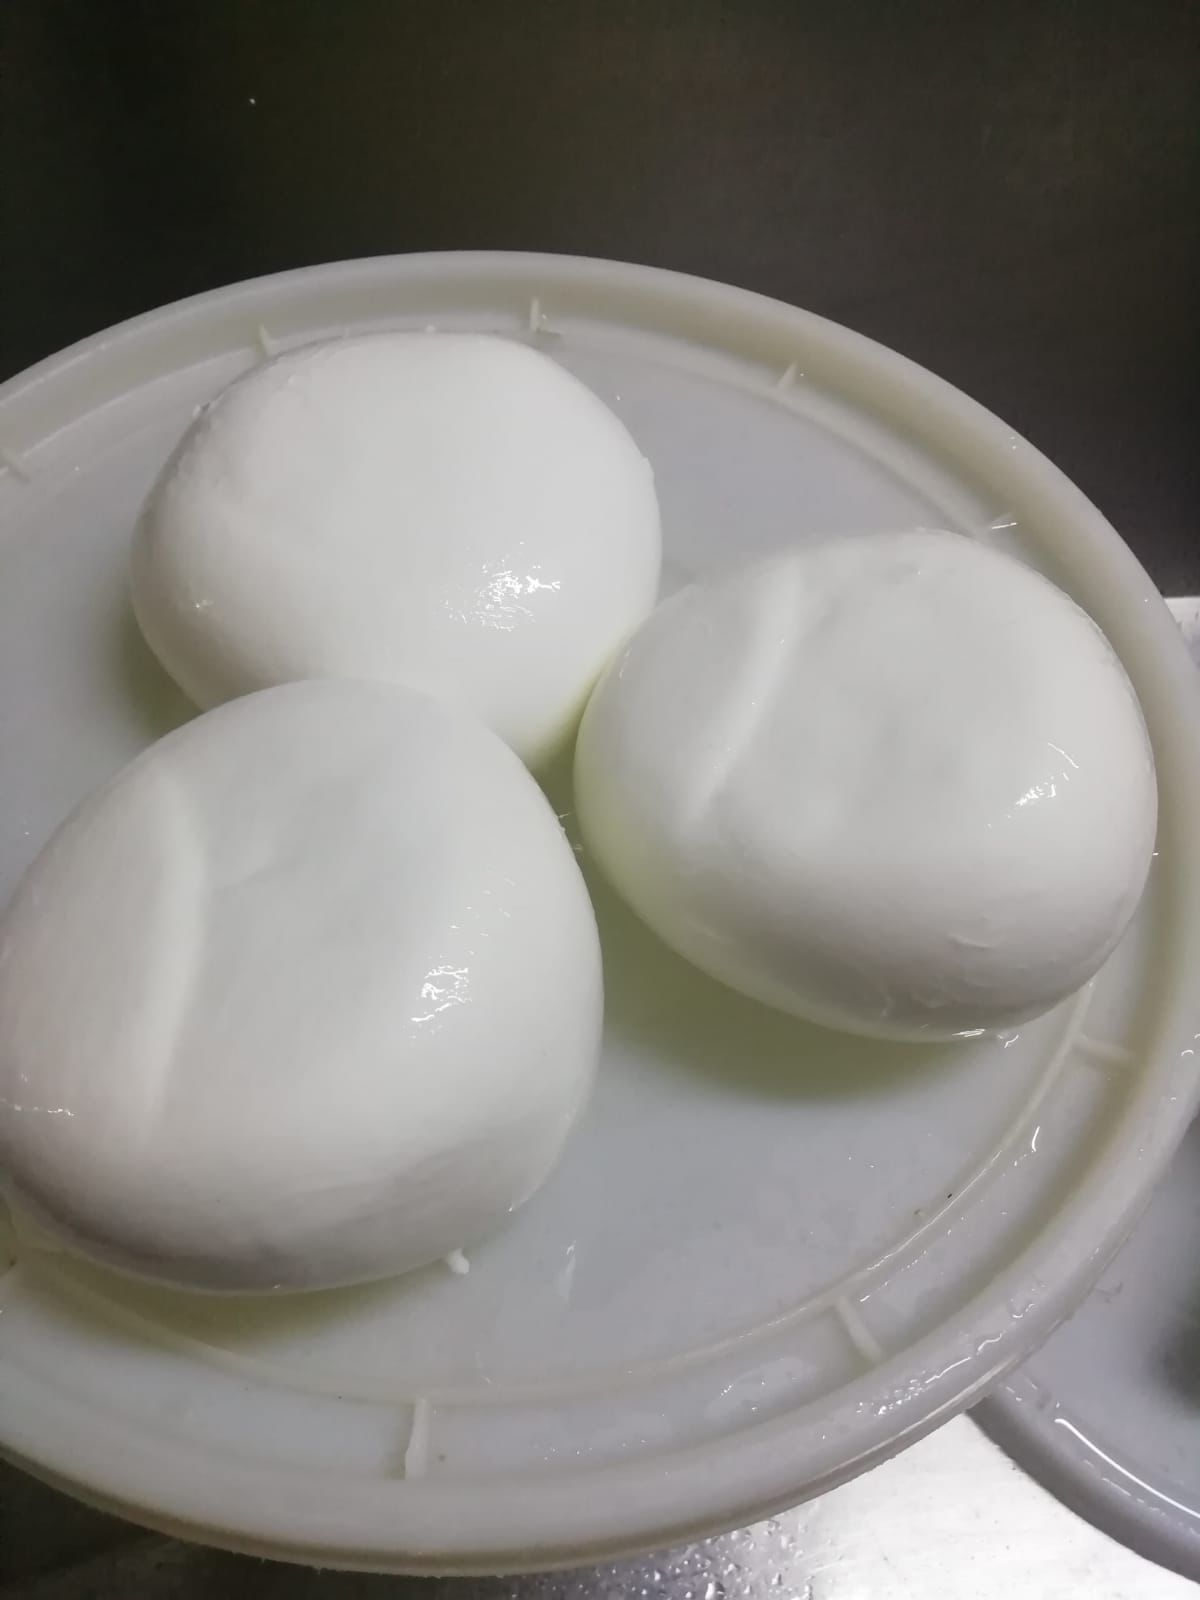
\includegraphics[scale=0.10]{imgs/photos/img1.jpeg}
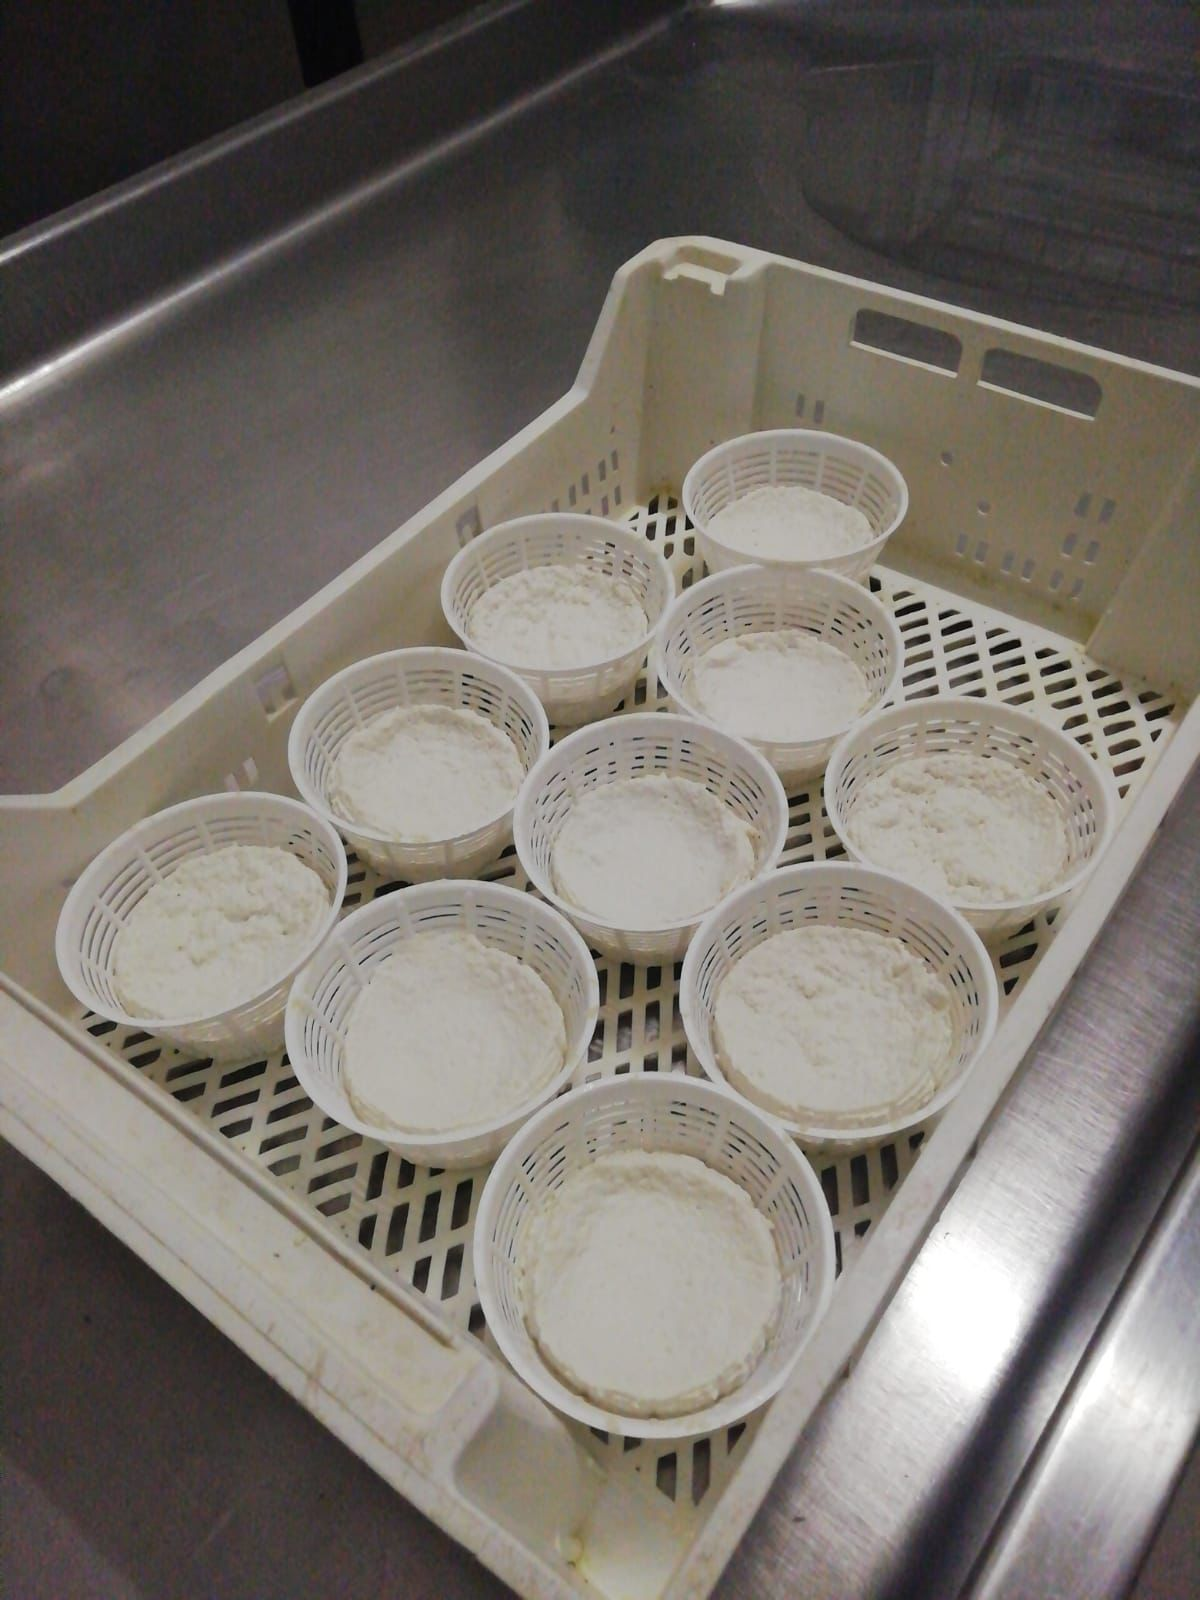
\includegraphics[scale=0.10]{imgs/photos/img2.jpeg}
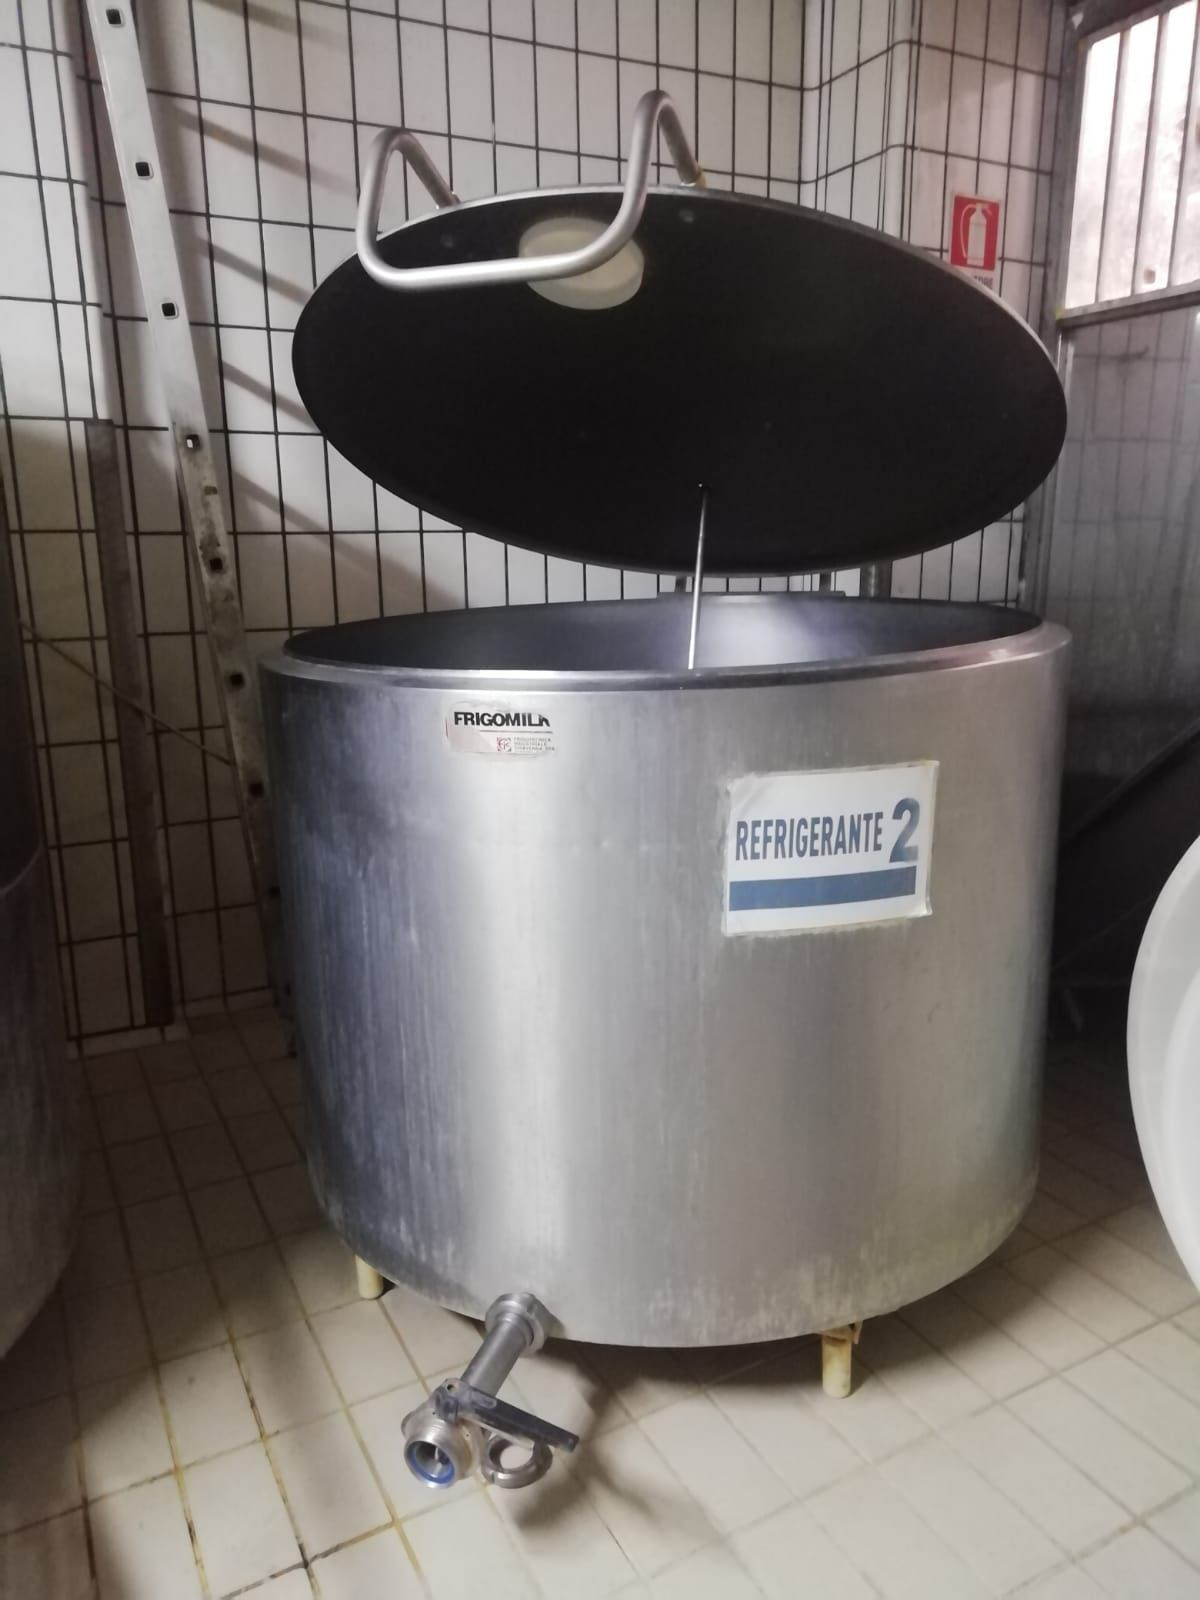
\includegraphics[scale=0.10]{imgs/photos/img3.jpeg}
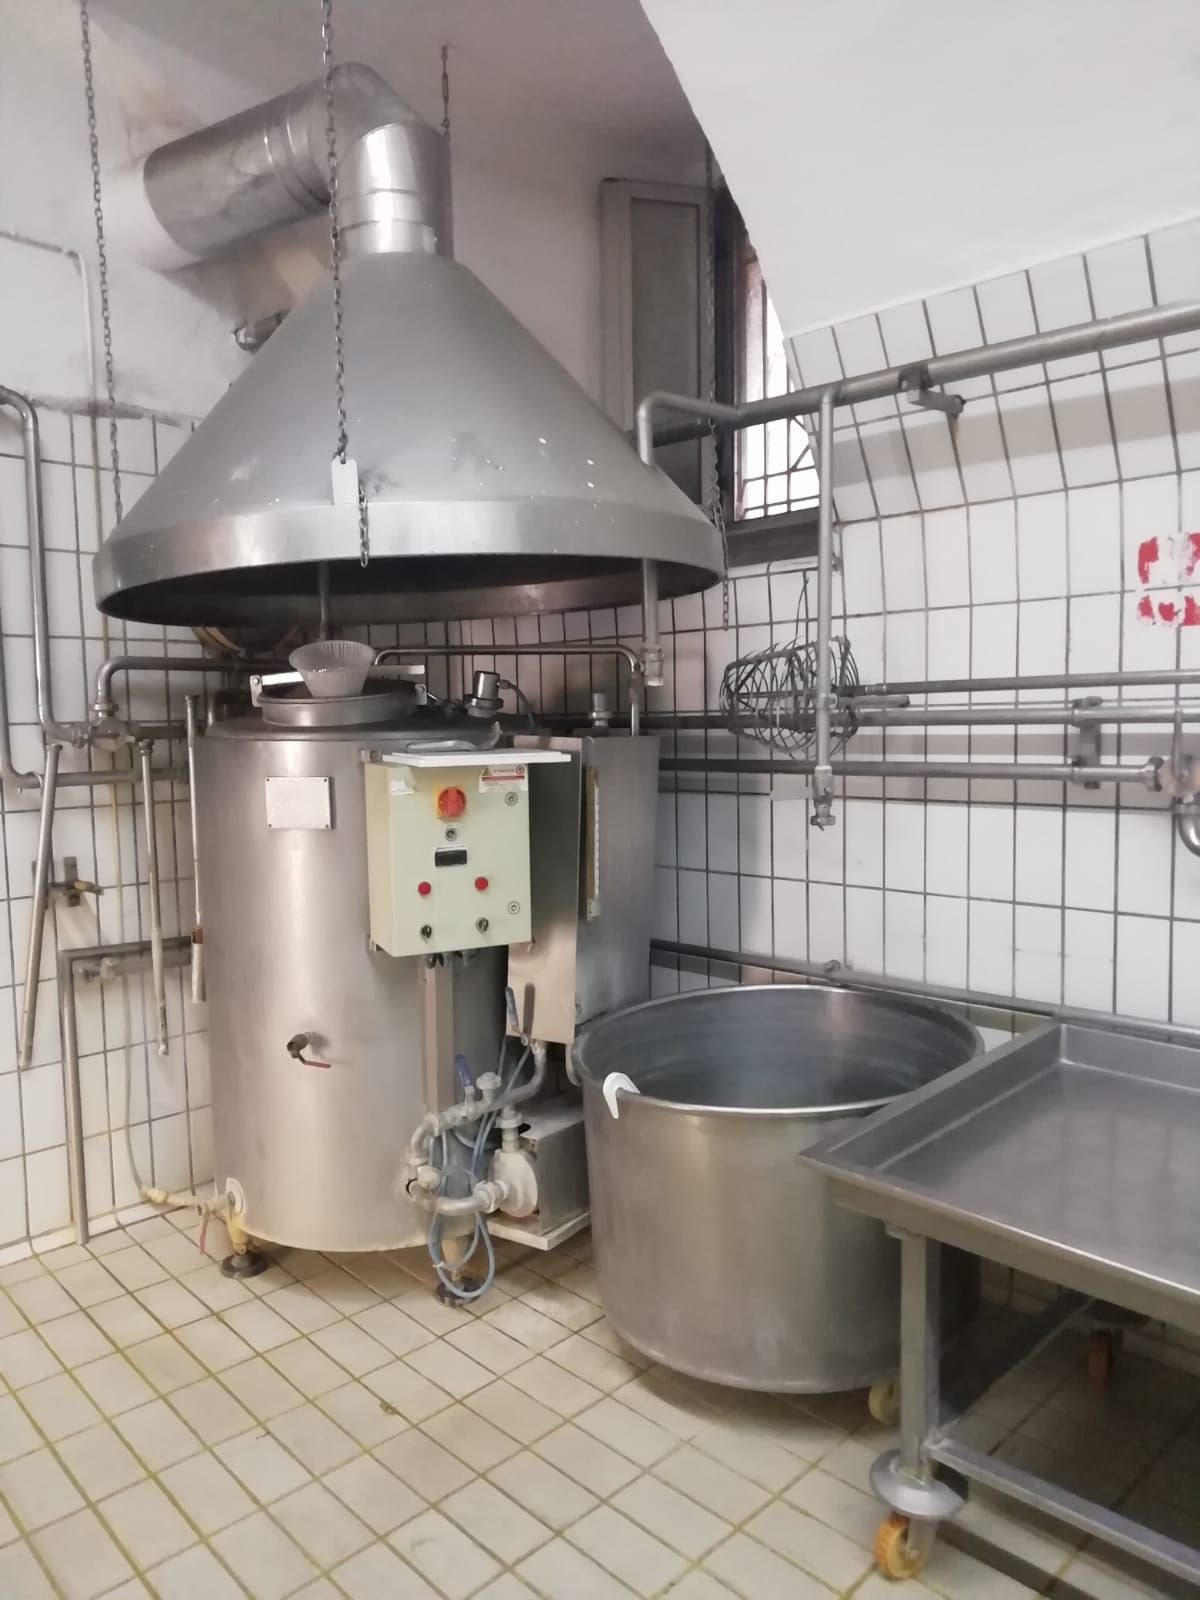
\includegraphics[scale=0.10]{imgs/photos/img4.jpeg}
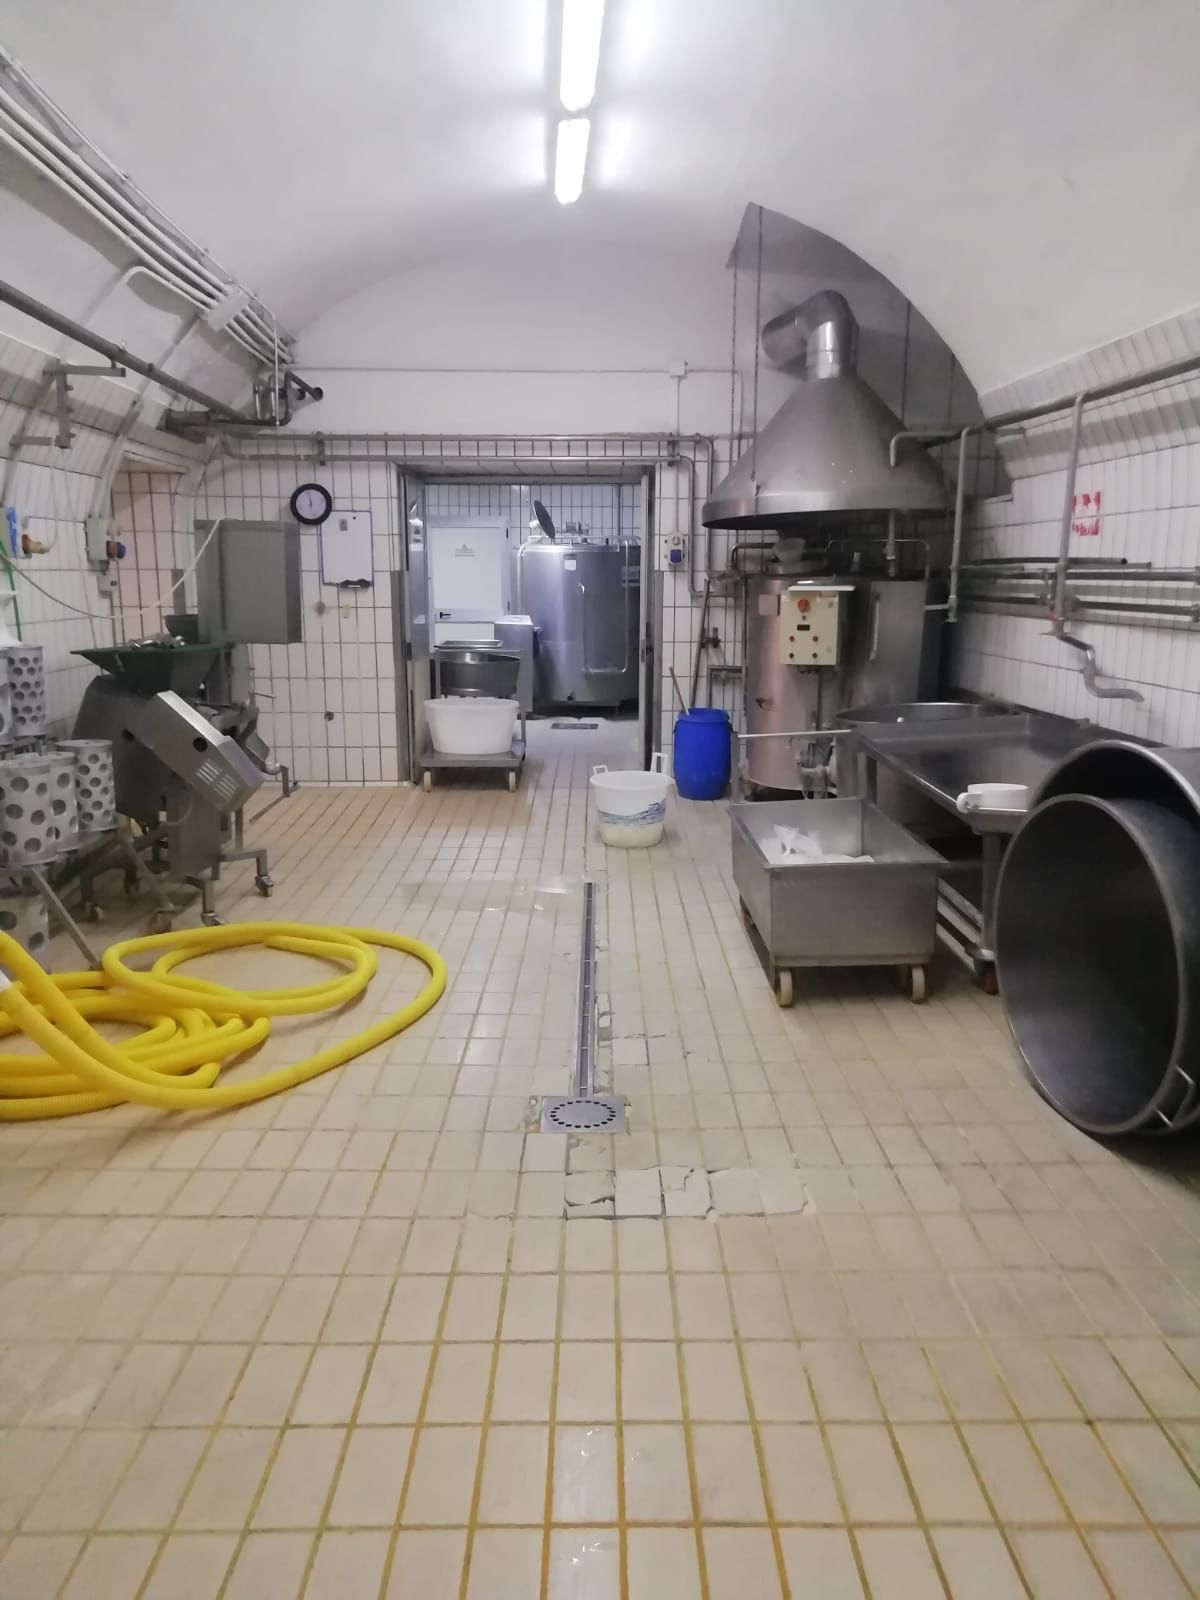
\includegraphics[scale=0.10]{imgs/photos/img5.jpeg}
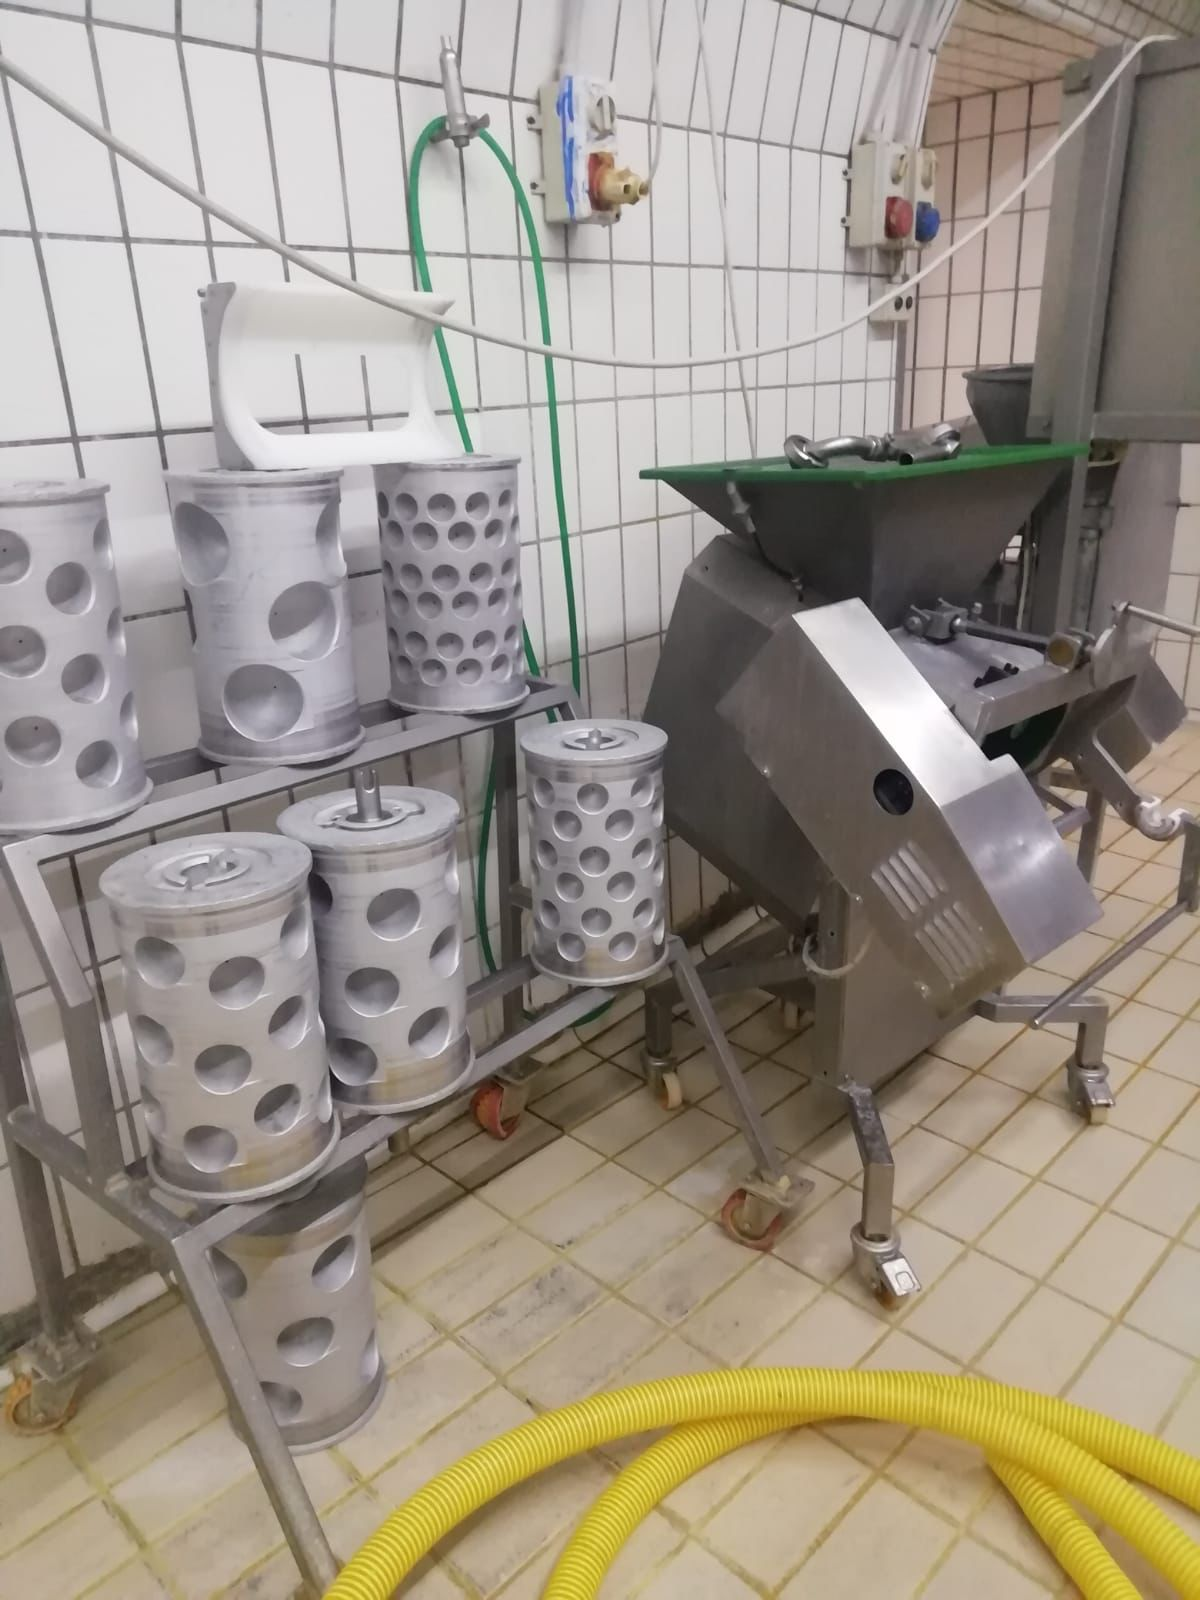
\includegraphics[scale=0.10]{imgs/photos/img6.jpeg}
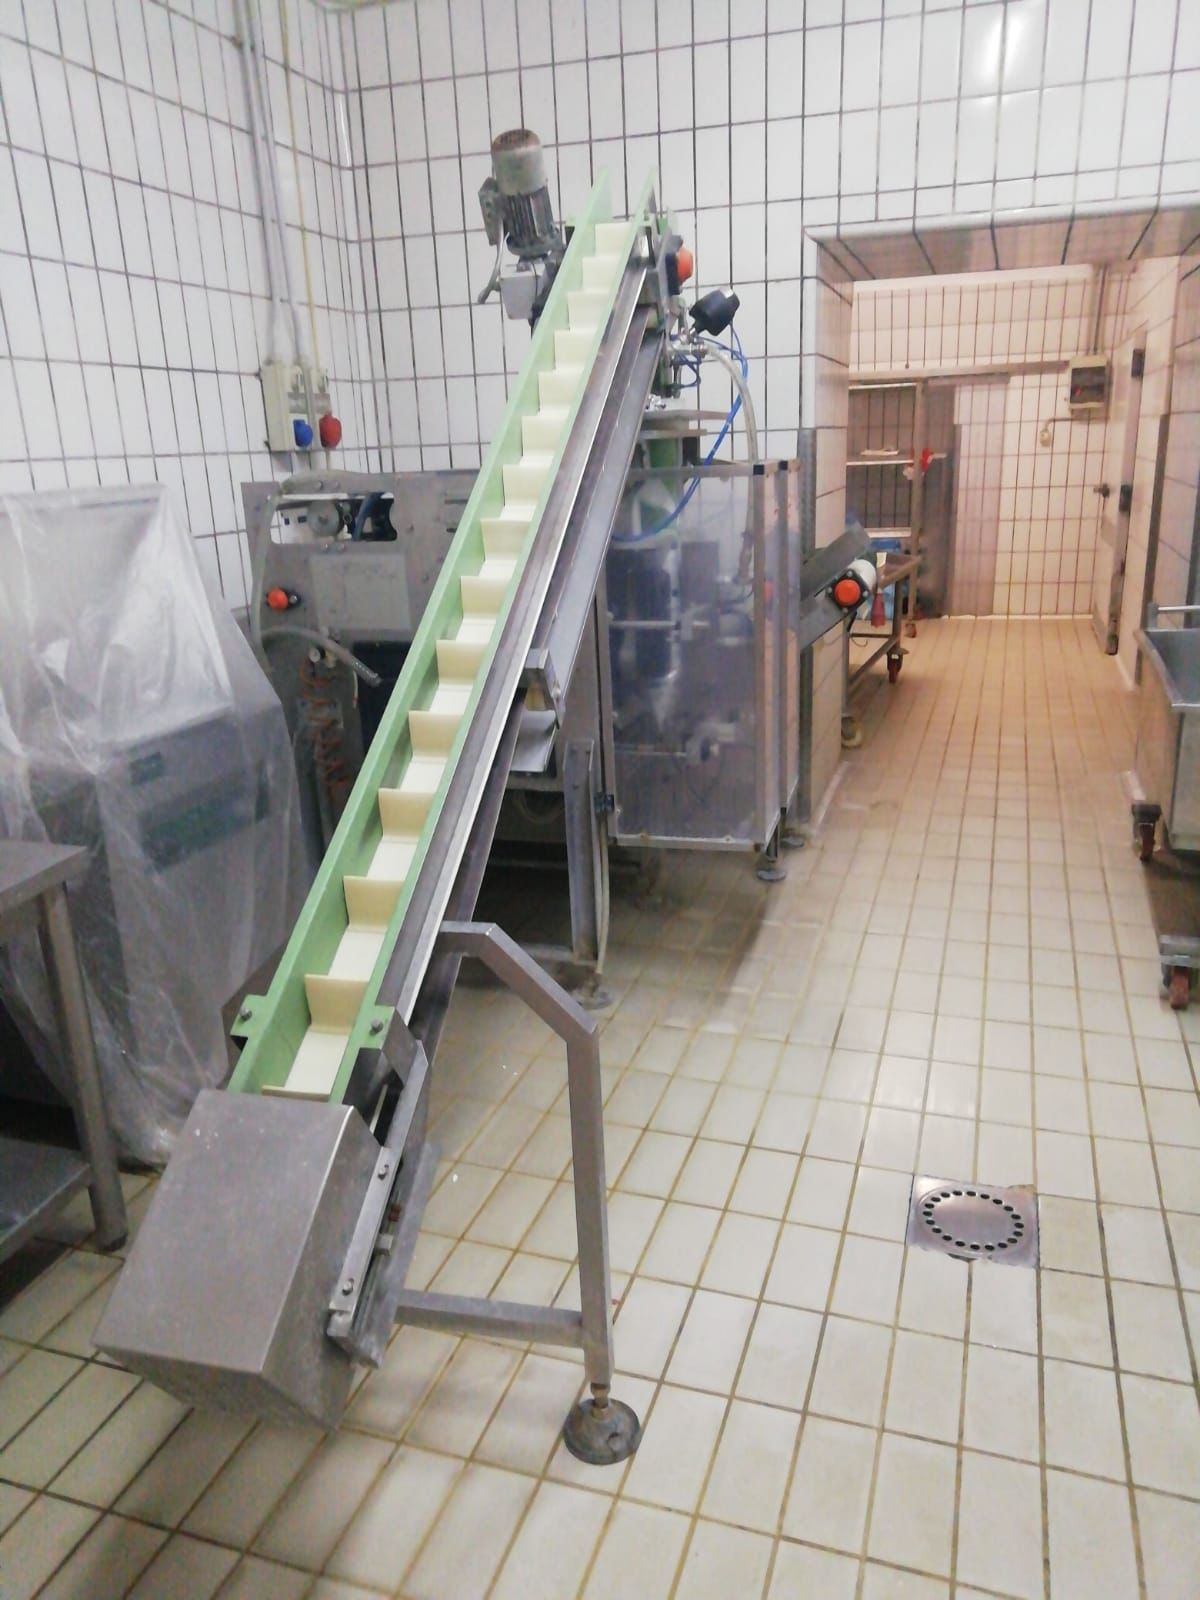
\includegraphics[scale=0.10]{imgs/photos/img7.jpeg}
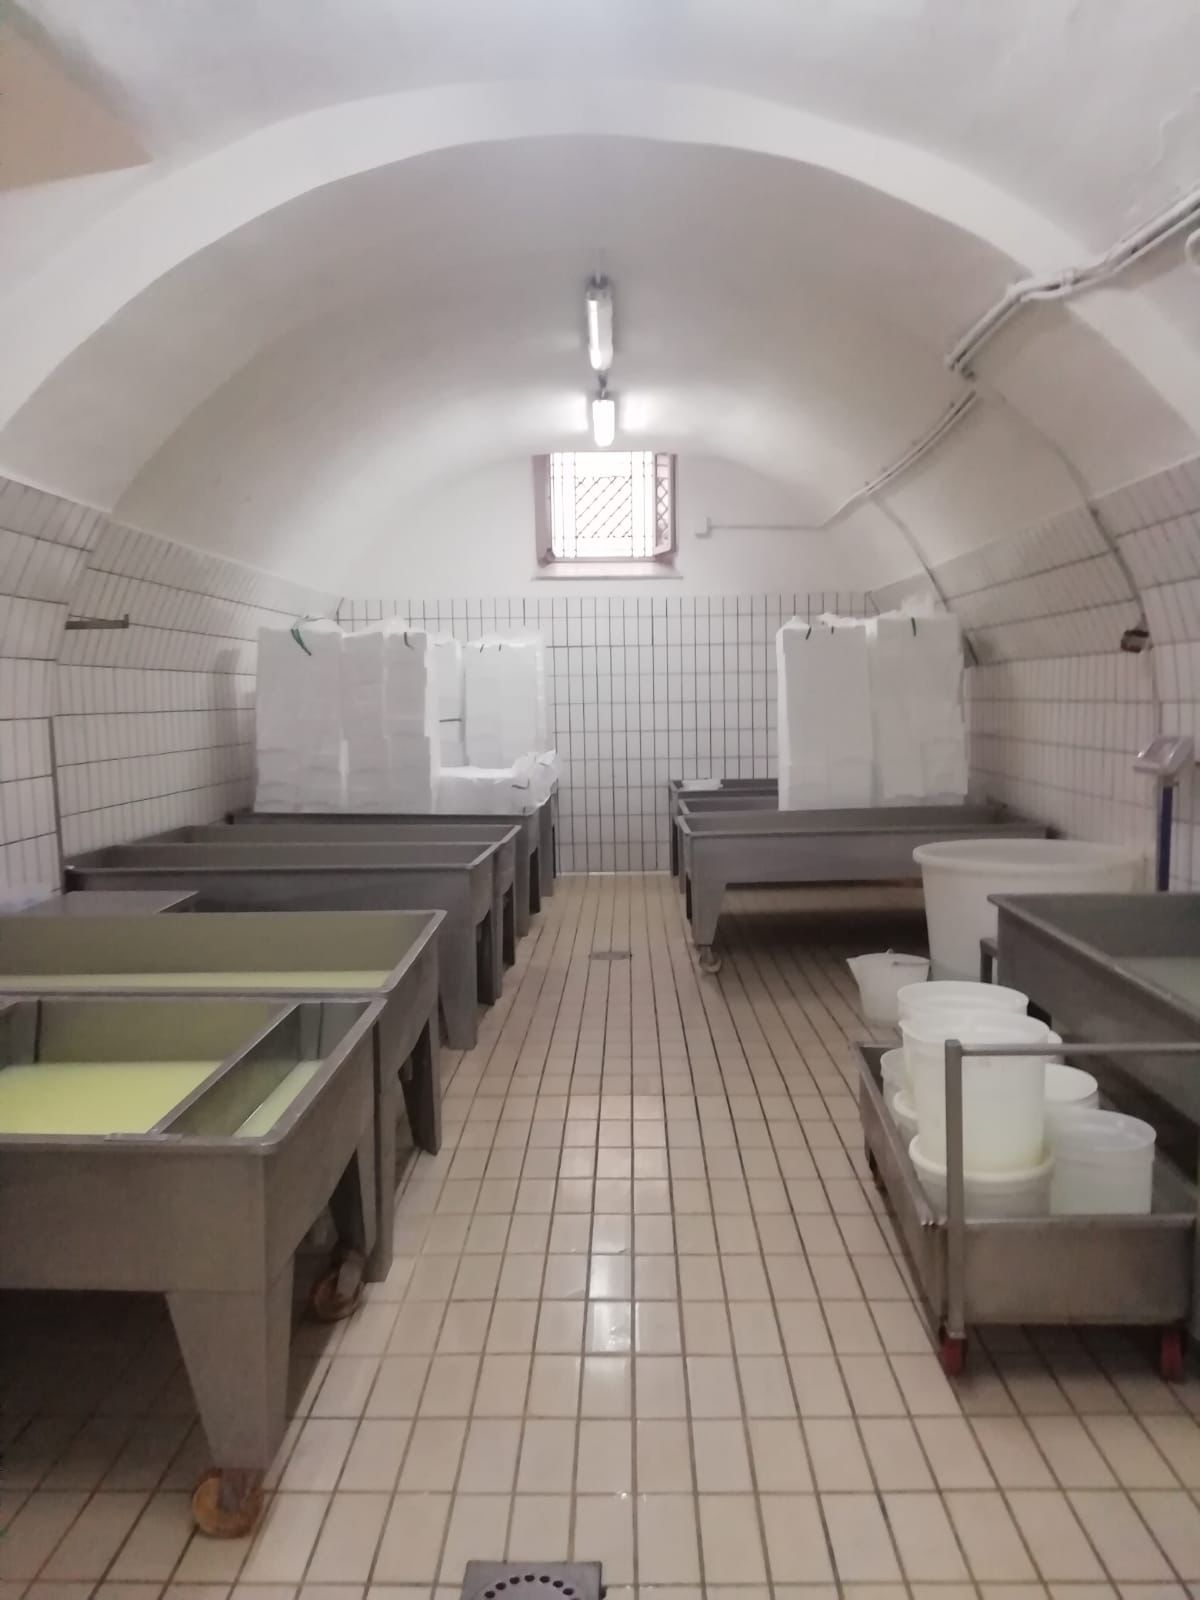
\includegraphics[scale=0.10]{imgs/photos/img8.jpeg}
\end{figure}


\chapter{Files Multimediali}
Di seguito sono illustrate tutte le cartelle coinvolte nel progetto. 
\section{Guida ai files multimediali}
\underline{Cartella}: \textbf{DOCUMENTAZIONE}
\begin{itemize}
\item Sorgente\_Relazione		\hspace{26mm} Cartella di File
\item Relazione\_Antica\_Casearia\_S.pdf
\end{itemize}
\underline{Cartella}: \textbf{DOCUMENTAZIONE > SORGENTE\_RELAZIONE}
\begin{itemize}
\item imgs		\hspace{53mm} Cartella di File
\item RELAZIONE.tex
\end{itemize}
\underline{Cartella}: \textbf{DOCUMENTAZIONE > SORGENTE\_RELAZIONE > imgs}
\begin{itemize}
\item photos        \hspace{49mm} Cartella di File
\item UML		    \hspace{52mm} Cartella di File
\item eer\_completo.jpeg
\item eer\_cliente.jpeg
\item eer\_dipendenti.jpeg
\item eer\_LabAnalisi.jpeg
\item eer\_veterinario.jpeg
\item sc\_relazionale.jpeg
\item logo.jpg
\end{itemize}
\underline{Cartella}: \textbf{DOCUMENTAZIONE > SORGENTE\_RELAZIONE > imgs > photos}
\begin{itemize}
\item img1.jpeg
\item img2.jpeg
\item img3.jpeg
\item img4.jpeg
\item img5.jpeg
\item img6.jpeg
\item img7.jpeg
\item img8.jpeg
\end{itemize}
\underline{Cartella}: \textbf{DOCUMENTAZIONE > SORGENTE\_RELAZIONE > imgs > UML}
\begin{itemize}
\item UML.jpeg
\item sdC\_SC.png
\item sdG\_TL.png
\item sdR\_CE.png
\item sdR\_TE.png
\item sdS\_CA.png
\item sdS\_VE.png
\end{itemize}

\underline{Cartella}: \textbf{IMPLEMENTAZIONE}
\begin{itemize}
\item CREAZIONE				\hspace{38mm} Cartella di File
\item PROCEDURE				\hspace{36mm} Cartella di File
\item QUICK\_BUILD			\hspace{33mm} Cartella di File
\item SCHEDULER				\hspace{36mm} Cartella di File
\item TRIGGER				\hspace{43mm} Cartella di File
\item UTENTI				\hspace{45mm} Cartella di File
\item VISTE					\hspace{49mm} Cartella di File
\end{itemize}
\underline{Cartella}: \textbf{IMPLEMENTAZIONE > CREAZIONE}
\begin{itemize}
\item CREATE\_TABLE.sql
\item DROP\_TABLE.sql
\item POPOLA\_TABELLE.sql
\end{itemize}
\underline{Cartella}: \textbf{IMPLEMENTAZIONE > PROCEDURE}
\begin{itemize}
\item CALCOLA\_SCONTO.sql
\item GENERA\_TURNO\_LAVORATIVO.sql
\item RINNOVO\_CERTIFICATO.sql
\item RINNOVO\_TESSERA.sql
\item SOSTITUISCI\_CASSIERE.sql
\item SOSTITUISCI\_VEICOLO.sql
\end{itemize}
\underline{Cartella}: \textbf{IMPLEMENTAZIONE > QUICK\_BUILD}
\begin{itemize}
\item \_INIT.sql
\item \_BUILD.sql
\item DROP\_UTENTI.sql
\item CREA\_UTENTI.sql
\item DROP\_TABLE.sql
\item DROP\_VIEW.sql
\item CREATE\_TABLE.sql
\item DCL\_UTENTI.sql
\item POPOLA\_TABELLE.sql
\item TR\_ANIMALE.sql
\item TR\_ASSISTE.sql
\item TR\_CONSEGNA.sql
\item TR\_LATTE.sql
\item TR\_PERSONA.sql
\item TR\_PRODOTTO.sql
\item TR\_PROMOZIONE.sql
\item TR\_TESSERA.sql
\item TR\_TURNOLAVORATIVO.sql
\item TR\_UTILIZZA.sql
\item CALCOLA\_SCONTO.sql
\item GENERA\_TURNO\_LAVORATIVO.sql
\item RINNOVO\_CERTIFICATO.sql
\item RINNOVO\_TESSERA.sql
\item SOSTITUISCI\_CASSIERE.sql
\item SOSTITUISCI\_VEICOLO.sql
\item CLASSIFICA\_CLIENTI.sql
\item ANDAMENTO\_PROMOZIONI.sql
\item REPORT\_VEICOLI.sql
\item TL\_DELETE\_DATA.sql
\item DROP\_TL\_DELETE\_DATA.sql
\end{itemize}
\underline{Cartella}: \textbf{IMPLEMENTAZIONE > SCHEDULER}
\begin{itemize}
\item TL\_DELETE\_DATA.sql
\item DROP\_TL\_DELETE\_DATA.sql
\end{itemize}
\underline{Cartella}: \textbf{IMPLEMENTAZIONE > TRIGGER}
\begin{itemize}
\item TR\_ANIMALE.sql
\item TR\_ASSISTE.sql
\item TR\_CONSEGNA.sql
\item TR\_LATTE.sql
\item TR\_PERSONA.sql
\item TR\_PRODOTTO.sql
\item TR\_PROMOZIONE.sql
\item TR\_TESSERA.sql
\item TR\_TURNOLAVORATIVO.sql
\item TR\_UTILIZZA.sql
\end{itemize}
\underline{Cartella}: \textbf{IMPLEMENTAZIONE > UTENTI}
\begin{itemize}
\item CREA\_UTENTI.sql
\item DCL\_UTENTI.sql
\item DROP\_UTENTI.sql
\end{itemize}
\underline{Cartella}: \textbf{IMPLEMENTAZIONE > VISTE}
\begin{itemize}
\item CLASSIFICA\_CLIENTI.sql
\item ANDAMENTO\_PROMOZIONI.sql
\item REPORT\_VEICOLI.sql
\item DROP\_VIEW.sql
\end{itemize}
\end{document}